%\documentclass[11pt]{book}
%
%\setlength{\parindent}{0pt}
%\setlength{\parskip}{8pt}
%
%\usepackage{amsmath}
%\usepackage{amssymb}
%\usepackage{hyperref}
%
%\renewcommand*{\thefootnote}{\fnsymbol{footnote}}
%
%\setcounter{chapter}{1}
%
%\begin{document}
%
%\section*{A Levelized Comparison of \\ Pulsed and Steady-State Tokamaks}
%
%\let\cleardoublepage\relax \tableofcontents \newpage

\chapter{Designing a Steady-State Tokamak}

This chapter explores a simple model for designing steady-state tokamaks. In the next couple chapters, the model is first formalized for use in a systems code and then generalized to handle pulsed operation. These derivations highlight that the only difference between the two modes is how they generate their auxiliary plasma current: LHCD for steady-state operation and inductive sources for when a reactor is purely pulsed.

Along the way, equations will be derived that get rather complicated. To remedy the situation, a distinction between floating and fixed values is now given, which will allow splitting most equations into fixed and floating parts. Fixed values -- i.e. the tokamak's major radius ($R_0$) and magnet strength ($B_0$), as well as the plasma's current ($I_P$), temperature ($\overline T$), and density ($\overline n$) -- are first-class variables in this model. Everything is derived to relate them. Fixed values, on the other hand, can be treated as code inputs, which remain constant throughout a reactor solve.  These most obviously include the various geometric and profile parameters introduced next section. 

\section{Defining Plasma Parameters}

As mentioned previously, the zero-dimensional model derived here can closely approximate solutions from higher-dimensional codes that might take weeks to run. The essence of boiling down three-dimensional behaviors to one dimensional profiles (and zero-dimensional averaged values) begins with defining the most important plasma parameters. These are the: current (J), temperature (T), and density (n) of a plasma.

Solving this problem most generally usually involves decoupling the geometry of the plasma from the shaping of nearly parabolic radial-profiles -- both of which will be explained shortly.

\subsection{Understanding Tokamak Geometry}

The first thing people see when they look at a tokamak is its geometry. How big is it? Is it stretched out like a tire or smooshed together like a bagel? If it were torn in two, would the exposed areas look like: circles, ovals, or triangles?

These questions lend themselves to the three important geometry variables -- the inverse aspect ratio ($\epsilon$), the elongation ($\kappa$), and the triangularity ($\delta$). The inverse aspect ratio is a measure of how stretched out the device is, or formulaically:

\begin{equation}
	\label{eq:a}
	a = \epsilon \cdot R_0
\end{equation}
\myequations{Minor Radius -- $a$}

This says that the minor radius (a), measured in meters, is related to the major radius of the machine ($R_0$) through $\epsilon$. More tangibly, the minor radius is related to the two small circles that come from tearing a bagel in two. The major radius is related to the overall circle of the bagel when viewing it from the top.

The remaining two geometric parameters -- $\kappa$ and $\delta$ -- are related to the shape of torn halves. As the name hints, elongation ($\kappa$) is a measure of how stretched out the tokamak is vertically -- is the cross-section a circle or an oval? The triangularity ($\delta$) is then how much the cross-sections point outward from the center of the device. All three's effects can be seen in \cref{fig:geometry}.

\begin{figure*}[h]
    \centering
    \hfill 
    \begin{subfigure}[t]{0.45\textwidth}
        \centering
		\begin{adjustbox}{width=\textwidth}
			\Large
			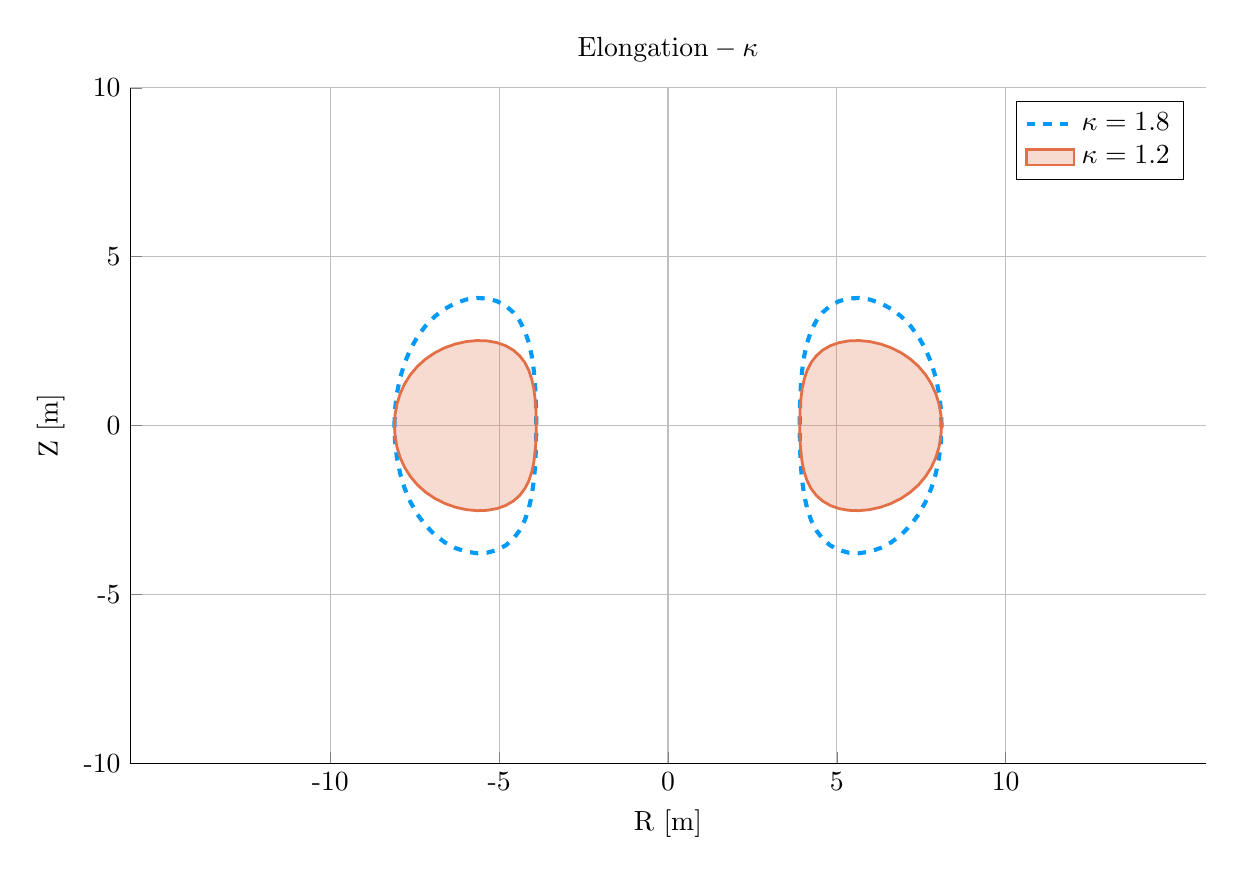
\begin{tikzpicture}[]
\begin{axis}[height = {101.6mm}, axis equal = {true}, ylabel = {Z [m]}, title = {$\textnormal{Elongation} - \kappa$}, xmin = {-10}, xmax = {10}, ymax = {10}, xlabel = {R [m]}, {unbounded coords=jump, scaled x ticks = false, xticklabel style={rotate = 0}, xmajorgrids = true, xtick = {-10.0,-5.0,0.0,5.0,10.0}, xticklabels = {-10,-5,0,5,10}, xtick align = inside, axis lines* = left, scaled y ticks = false, yticklabel style={rotate = 0}, ymajorgrids = true, ytick = {-10.0,-5.0,0.0,5.0,10.0}, yticklabels = {-10,-5,0,5,10}, ytick align = inside, axis lines* = left,     xshift = 0.0mm,
    yshift = 0.0mm,
    axis background/.style={fill={rgb,1:red,1.00000000;green,1.00000000;blue,1.00000000}}
}, ymin = {-10}, width = {152.4mm}]\addplot+ [color = {rgb,1:red,0.00000000;green,0.60560316;blue,0.97868012},
draw opacity=1.0,
line width=1.5,
dashed,mark = none,
mark size = 2.0,
mark options = {
    color = {rgb,1:red,0.00000000;green,0.00000000;blue,0.00000000}, draw opacity = 1.0,
    fill = {rgb,1:red,0.00000000;green,0.60560316;blue,0.97868012}, fill opacity = 1.0,
    line width = 1,
    rotate = 0,
    solid
}]coordinates {
(8.1, 0.0)
(8.081204069972497, 0.48337567116743263)
(8.024684777757766, 0.9588143271779377)
(7.930141280572084, 1.4185092784440338)
(7.797367695668915, 1.854912346574885)
(7.626640572703316, 2.260857805256796)
(7.419158721180681, 2.6296800412811785)
(7.177452352825953, 2.9553230037291525)
(6.905679431512412, 3.232439644160208)
(6.609741255084048, 3.456479714999771)
(6.297174663233395, 3.623764484478577)
(5.976811190071814, 3.7315471413066206)
(5.658229090447864, 3.7780578972385994)
(5.351057127458824, 3.7625330469479685)
(5.06421429716898, 3.685227508047293)
(4.805183334632925, 3.547410635348094)
(4.579415603765742, 3.3513453780899396)
(4.389950548568067, 3.100251122376493)
(4.237306076467235, 2.7982508289446923)
(4.119660690046763, 2.45030333426344)
(4.033308834588962, 2.0621219265758737)
(3.9733333500050683, 1.6400805338643698)
(3.9344084806536994, 1.1911090641292867)
(3.911628010194501, 0.7225796164911881)
(3.9012485454184915, 0.24218543152709598)
(3.9012485454184915, -0.2421854315270951)
(3.911628010194501, -0.7225796164911872)
(3.9344084806536994, -1.1911090641292859)
(3.9733333500050687, -1.640080533864369)
(4.033308834588962, -2.0621219265758732)
(4.119660690046763, -2.450303334263439)
(4.237306076467235, -2.7982508289446915)
(4.389950548568066, -3.1002511223764917)
(4.579415603765742, -3.3513453780899396)
(4.8051833346329245, -3.5474106353480934)
(5.064214297168979, -3.685227508047293)
(5.351057127458825, -3.7625330469479685)
(5.658229090447862, -3.7780578972385994)
(5.976811190071814, -3.731547141306621)
(6.297174663233394, -3.6237644844785772)
(6.609741255084048, -3.456479714999771)
(6.90567943151241, -3.232439644160209)
(7.177452352825952, -2.955323003729153)
(7.419158721180681, -2.629680041281178)
(7.626640572703316, -2.260857805256797)
(7.797367695668915, -1.854912346574885)
(7.930141280572083, -1.4185092784440358)
(8.024684777757766, -0.9588143271779382)
(8.081204069972497, -0.483375671167435)
(8.1, -9.258329801553988e-16)
};
\addlegendentry{$\kappa = 1.8$}
\addplot+ [color = {rgb,1:red,0.00000000;green,0.60560316;blue,0.97868012},
draw opacity=1.0,
line width=1.5,
dashed,mark = none,
mark size = 2.0,
mark options = {
    color = {rgb,1:red,0.00000000;green,0.00000000;blue,0.00000000}, draw opacity = 1.0,
    fill = {rgb,1:red,0.00000000;green,0.60560316;blue,0.97868012}, fill opacity = 1.0,
    line width = 1,
    rotate = 0,
    solid
},forget plot]coordinates {
(-8.1, 0.0)
(-8.081204069972497, 0.48337567116743263)
(-8.024684777757766, 0.9588143271779377)
(-7.930141280572084, 1.4185092784440338)
(-7.797367695668915, 1.854912346574885)
(-7.626640572703316, 2.260857805256796)
(-7.419158721180681, 2.6296800412811785)
(-7.177452352825953, 2.9553230037291525)
(-6.905679431512412, 3.232439644160208)
(-6.609741255084048, 3.456479714999771)
(-6.297174663233395, 3.623764484478577)
(-5.976811190071814, 3.7315471413066206)
(-5.658229090447864, 3.7780578972385994)
(-5.351057127458824, 3.7625330469479685)
(-5.06421429716898, 3.685227508047293)
(-4.805183334632925, 3.547410635348094)
(-4.579415603765742, 3.3513453780899396)
(-4.389950548568067, 3.100251122376493)
(-4.237306076467235, 2.7982508289446923)
(-4.119660690046763, 2.45030333426344)
(-4.033308834588962, 2.0621219265758737)
(-3.9733333500050683, 1.6400805338643698)
(-3.9344084806536994, 1.1911090641292867)
(-3.911628010194501, 0.7225796164911881)
(-3.9012485454184915, 0.24218543152709598)
(-3.9012485454184915, -0.2421854315270951)
(-3.911628010194501, -0.7225796164911872)
(-3.9344084806536994, -1.1911090641292859)
(-3.9733333500050687, -1.640080533864369)
(-4.033308834588962, -2.0621219265758732)
(-4.119660690046763, -2.450303334263439)
(-4.237306076467235, -2.7982508289446915)
(-4.389950548568066, -3.1002511223764917)
(-4.579415603765742, -3.3513453780899396)
(-4.8051833346329245, -3.5474106353480934)
(-5.064214297168979, -3.685227508047293)
(-5.351057127458825, -3.7625330469479685)
(-5.658229090447862, -3.7780578972385994)
(-5.976811190071814, -3.731547141306621)
(-6.297174663233394, -3.6237644844785772)
(-6.609741255084048, -3.456479714999771)
(-6.90567943151241, -3.232439644160209)
(-7.177452352825952, -2.955323003729153)
(-7.419158721180681, -2.629680041281178)
(-7.626640572703316, -2.260857805256797)
(-7.797367695668915, -1.854912346574885)
(-7.930141280572083, -1.4185092784440358)
(-8.024684777757766, -0.9588143271779382)
(-8.081204069972497, -0.483375671167435)
(-8.1, -9.258329801553988e-16)
};
\addplot+ [color = {rgb,1:red,0.88887350;green,0.43564919;blue,0.27812294},
draw opacity=1.0,
line width=1,
solid,mark = none,
mark size = 2.0,
mark options = {
    color = {rgb,1:red,0.00000000;green,0.00000000;blue,0.00000000}, draw opacity = 1.0,
    fill = {rgb,1:red,0.88887350;green,0.43564919;blue,0.27812294}, fill opacity = 1.0,
    line width = 1,
    rotate = 0,
    solid
},fill = {rgb,1:red,0.88887350;green,0.43564919;blue,0.27812294}, fill opacity=0.25,area legend]coordinates {
(8.1, 0.0)
(8.081204069972497, 0.322250447444955)
(8.024684777757766, 0.6392095514519583)
(7.930141280572084, 0.9456728522960225)
(7.797367695668915, 1.2366082310499231)
(7.626640572703316, 1.507238536837864)
(7.419158721180681, 1.7531200275207854)
(7.177452352825953, 1.9702153358194345)
(6.905679431512412, 2.1549597627734713)
(6.609741255084048, 2.304319809999847)
(6.297174663233395, 2.415842989652384)
(5.976811190071814, 2.487698094204414)
(5.658229090447864, 2.518705264825733)
(5.351057127458824, 2.508355364631979)
(5.06421429716898, 2.456818338698195)
(4.805183334632925, 2.364940423565396)
(4.579415603765742, 2.2342302520599597)
(4.389950548568067, 2.0668340815843287)
(4.237306076467235, 1.8655005526297948)
(4.119660690046763, 1.6335355561756264)
(4.033308834588962, 1.3747479510505825)
(3.9733333500050683, 1.0933870225762463)
(3.9344084806536994, 0.7940727094195245)
(3.911628010194501, 0.48171974432745873)
(3.9012485454184915, 0.16145695435139729)
(3.9012485454184915, -0.1614569543513967)
(3.911628010194501, -0.48171974432745807)
(3.9344084806536994, -0.7940727094195238)
(3.9733333500050687, -1.0933870225762459)
(4.033308834588962, -1.3747479510505818)
(4.119660690046763, -1.633535556175626)
(4.237306076467235, -1.8655005526297943)
(4.389950548568066, -2.066834081584328)
(4.579415603765742, -2.2342302520599593)
(4.8051833346329245, -2.3649404235653955)
(5.064214297168979, -2.456818338698195)
(5.351057127458825, -2.508355364631979)
(5.658229090447862, -2.518705264825733)
(5.976811190071814, -2.487698094204414)
(6.297174663233394, -2.415842989652385)
(6.609741255084048, -2.304319809999847)
(6.90567943151241, -2.1549597627734722)
(7.177452352825952, -1.9702153358194348)
(7.419158721180681, -1.7531200275207852)
(7.626640572703316, -1.5072385368378645)
(7.797367695668915, -1.2366082310499231)
(7.930141280572083, -0.9456728522960237)
(8.024684777757766, -0.6392095514519588)
(8.081204069972497, -0.3222504474449567)
(8.1, -6.172219867702659e-16)
};
\addlegendentry{$\kappa = 1.2$}
\addplot+ [color = {rgb,1:red,0.88887350;green,0.43564919;blue,0.27812294},
draw opacity=1.0,
line width=1,
solid,mark = none,
mark size = 2.0,
mark options = {
    color = {rgb,1:red,0.00000000;green,0.00000000;blue,0.00000000}, draw opacity = 1.0,
    fill = {rgb,1:red,0.88887350;green,0.43564919;blue,0.27812294}, fill opacity = 1.0,
    line width = 1,
    rotate = 0,
    solid
},fill = {rgb,1:red,0.88887350;green,0.43564919;blue,0.27812294}, fill opacity=0.25,forget plot]coordinates {
(-8.1, 0.0)
(-8.081204069972497, 0.322250447444955)
(-8.024684777757766, 0.6392095514519583)
(-7.930141280572084, 0.9456728522960225)
(-7.797367695668915, 1.2366082310499231)
(-7.626640572703316, 1.507238536837864)
(-7.419158721180681, 1.7531200275207854)
(-7.177452352825953, 1.9702153358194345)
(-6.905679431512412, 2.1549597627734713)
(-6.609741255084048, 2.304319809999847)
(-6.297174663233395, 2.415842989652384)
(-5.976811190071814, 2.487698094204414)
(-5.658229090447864, 2.518705264825733)
(-5.351057127458824, 2.508355364631979)
(-5.06421429716898, 2.456818338698195)
(-4.805183334632925, 2.364940423565396)
(-4.579415603765742, 2.2342302520599597)
(-4.389950548568067, 2.0668340815843287)
(-4.237306076467235, 1.8655005526297948)
(-4.119660690046763, 1.6335355561756264)
(-4.033308834588962, 1.3747479510505825)
(-3.9733333500050683, 1.0933870225762463)
(-3.9344084806536994, 0.7940727094195245)
(-3.911628010194501, 0.48171974432745873)
(-3.9012485454184915, 0.16145695435139729)
(-3.9012485454184915, -0.1614569543513967)
(-3.911628010194501, -0.48171974432745807)
(-3.9344084806536994, -0.7940727094195238)
(-3.9733333500050687, -1.0933870225762459)
(-4.033308834588962, -1.3747479510505818)
(-4.119660690046763, -1.633535556175626)
(-4.237306076467235, -1.8655005526297943)
(-4.389950548568066, -2.066834081584328)
(-4.579415603765742, -2.2342302520599593)
(-4.8051833346329245, -2.3649404235653955)
(-5.064214297168979, -2.456818338698195)
(-5.351057127458825, -2.508355364631979)
(-5.658229090447862, -2.518705264825733)
(-5.976811190071814, -2.487698094204414)
(-6.297174663233394, -2.415842989652385)
(-6.609741255084048, -2.304319809999847)
(-6.90567943151241, -2.1549597627734722)
(-7.177452352825952, -1.9702153358194348)
(-7.419158721180681, -1.7531200275207852)
(-7.626640572703316, -1.5072385368378645)
(-7.797367695668915, -1.2366082310499231)
(-7.930141280572083, -0.9456728522960237)
(-8.024684777757766, -0.6392095514519588)
(-8.081204069972497, -0.3222504474449567)
(-8.1, -6.172219867702659e-16)
};
\end{axis}

\end{tikzpicture}

		\end{adjustbox}
        \caption{$\kappa$}
    \end{subfigure}
    \hfill
    \begin{subfigure}[t]{0.45\textwidth}
        \centering
		\begin{adjustbox}{width=\textwidth}
			\Large
			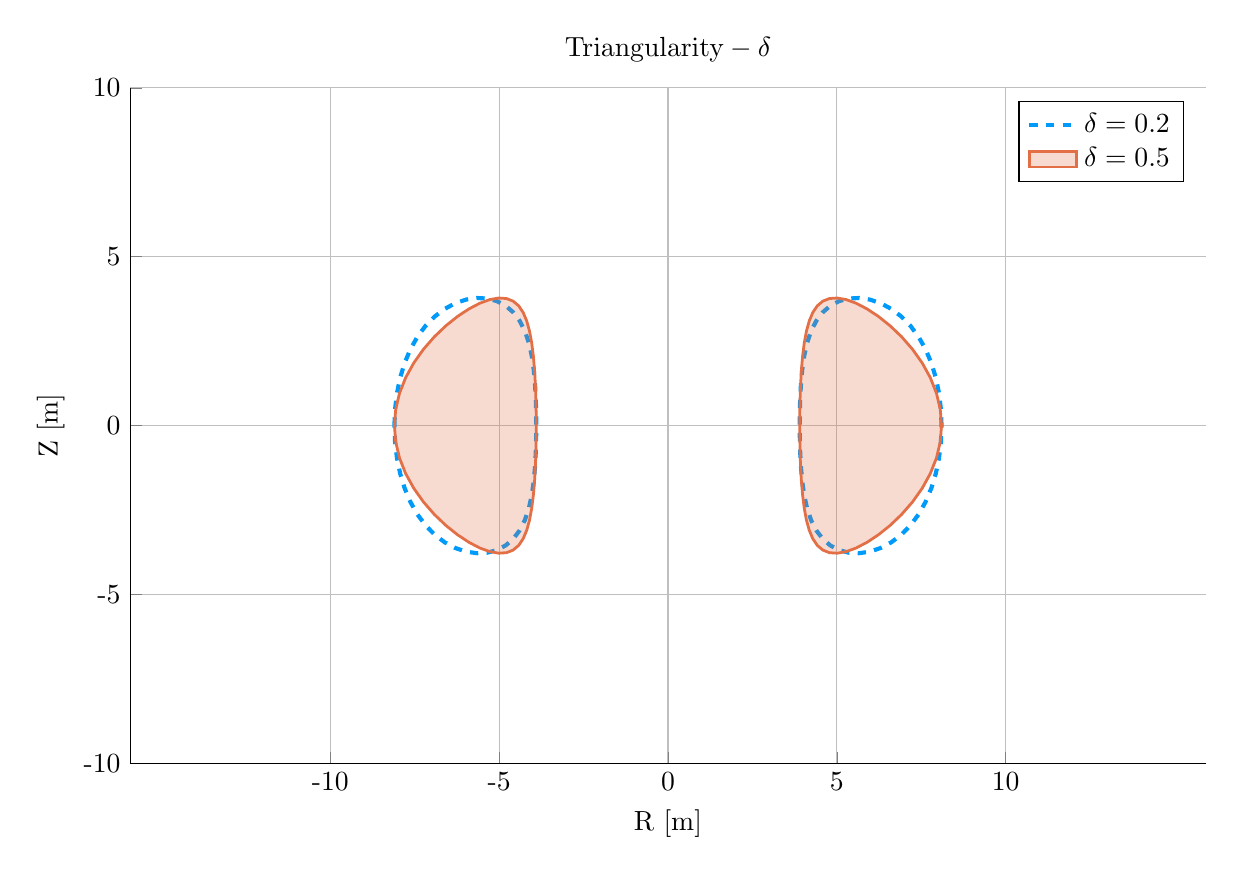
\begin{tikzpicture}[]
\begin{axis}[height = {101.6mm}, axis equal = {true}, ylabel = {Z [m]}, title = {$\textnormal{Triangularity} - \delta$}, xmin = {-10}, xmax = {10}, ymax = {10}, xlabel = {R [m]}, {unbounded coords=jump, scaled x ticks = false, xticklabel style={rotate = 0}, xmajorgrids = true, xtick = {-10.0,-5.0,0.0,5.0,10.0}, xticklabels = {-10,-5,0,5,10}, xtick align = inside, axis lines* = left, scaled y ticks = false, yticklabel style={rotate = 0}, ymajorgrids = true, ytick = {-10.0,-5.0,0.0,5.0,10.0}, yticklabels = {-10,-5,0,5,10}, ytick align = inside, axis lines* = left,     xshift = 0.0mm,
    yshift = 0.0mm,
    axis background/.style={fill={rgb,1:red,1.00000000;green,1.00000000;blue,1.00000000}}
}, ymin = {-10}, width = {152.4mm}]\addplot+ [color = {rgb,1:red,0.00000000;green,0.60560316;blue,0.97868012},
draw opacity=1.0,
line width=1.5,
dashed,mark = none,
mark size = 2.0,
mark options = {
    color = {rgb,1:red,0.00000000;green,0.00000000;blue,0.00000000}, draw opacity = 1.0,
    fill = {rgb,1:red,0.00000000;green,0.60560316;blue,0.97868012}, fill opacity = 1.0,
    line width = 1,
    rotate = 0,
    solid
}]coordinates {
(8.1, 0.0)
(8.081204069972497, 0.48337567116743263)
(8.024684777757766, 0.9588143271779377)
(7.930141280572084, 1.4185092784440338)
(7.797367695668915, 1.854912346574885)
(7.626640572703316, 2.260857805256796)
(7.419158721180681, 2.6296800412811785)
(7.177452352825953, 2.9553230037291525)
(6.905679431512412, 3.232439644160208)
(6.609741255084048, 3.456479714999771)
(6.297174663233395, 3.623764484478577)
(5.976811190071814, 3.7315471413066206)
(5.658229090447864, 3.7780578972385994)
(5.351057127458824, 3.7625330469479685)
(5.06421429716898, 3.685227508047293)
(4.805183334632925, 3.547410635348094)
(4.579415603765742, 3.3513453780899396)
(4.389950548568067, 3.100251122376493)
(4.237306076467235, 2.7982508289446923)
(4.119660690046763, 2.45030333426344)
(4.033308834588962, 2.0621219265758737)
(3.9733333500050683, 1.6400805338643698)
(3.9344084806536994, 1.1911090641292867)
(3.911628010194501, 0.7225796164911881)
(3.9012485454184915, 0.24218543152709598)
(3.9012485454184915, -0.2421854315270951)
(3.911628010194501, -0.7225796164911872)
(3.9344084806536994, -1.1911090641292859)
(3.9733333500050687, -1.640080533864369)
(4.033308834588962, -2.0621219265758732)
(4.119660690046763, -2.450303334263439)
(4.237306076467235, -2.7982508289446915)
(4.389950548568066, -3.1002511223764917)
(4.579415603765742, -3.3513453780899396)
(4.8051833346329245, -3.5474106353480934)
(5.064214297168979, -3.685227508047293)
(5.351057127458825, -3.7625330469479685)
(5.658229090447862, -3.7780578972385994)
(5.976811190071814, -3.731547141306621)
(6.297174663233394, -3.6237644844785772)
(6.609741255084048, -3.456479714999771)
(6.90567943151241, -3.232439644160209)
(7.177452352825952, -2.955323003729153)
(7.419158721180681, -2.629680041281178)
(7.626640572703316, -2.260857805256797)
(7.797367695668915, -1.854912346574885)
(7.930141280572083, -1.4185092784440358)
(8.024684777757766, -0.9588143271779382)
(8.081204069972497, -0.483375671167435)
(8.1, -9.258329801553988e-16)
};
\addlegendentry{$\delta = 0.2$}
\addplot+ [color = {rgb,1:red,0.00000000;green,0.60560316;blue,0.97868012},
draw opacity=1.0,
line width=1.5,
dashed,mark = none,
mark size = 2.0,
mark options = {
    color = {rgb,1:red,0.00000000;green,0.00000000;blue,0.00000000}, draw opacity = 1.0,
    fill = {rgb,1:red,0.00000000;green,0.60560316;blue,0.97868012}, fill opacity = 1.0,
    line width = 1,
    rotate = 0,
    solid
},forget plot]coordinates {
(-8.1, 0.0)
(-8.081204069972497, 0.48337567116743263)
(-8.024684777757766, 0.9588143271779377)
(-7.930141280572084, 1.4185092784440338)
(-7.797367695668915, 1.854912346574885)
(-7.626640572703316, 2.260857805256796)
(-7.419158721180681, 2.6296800412811785)
(-7.177452352825953, 2.9553230037291525)
(-6.905679431512412, 3.232439644160208)
(-6.609741255084048, 3.456479714999771)
(-6.297174663233395, 3.623764484478577)
(-5.976811190071814, 3.7315471413066206)
(-5.658229090447864, 3.7780578972385994)
(-5.351057127458824, 3.7625330469479685)
(-5.06421429716898, 3.685227508047293)
(-4.805183334632925, 3.547410635348094)
(-4.579415603765742, 3.3513453780899396)
(-4.389950548568067, 3.100251122376493)
(-4.237306076467235, 2.7982508289446923)
(-4.119660690046763, 2.45030333426344)
(-4.033308834588962, 2.0621219265758737)
(-3.9733333500050683, 1.6400805338643698)
(-3.9344084806536994, 1.1911090641292867)
(-3.911628010194501, 0.7225796164911881)
(-3.9012485454184915, 0.24218543152709598)
(-3.9012485454184915, -0.2421854315270951)
(-3.911628010194501, -0.7225796164911872)
(-3.9344084806536994, -1.1911090641292859)
(-3.9733333500050687, -1.640080533864369)
(-4.033308834588962, -2.0621219265758732)
(-4.119660690046763, -2.450303334263439)
(-4.237306076467235, -2.7982508289446915)
(-4.389950548568066, -3.1002511223764917)
(-4.579415603765742, -3.3513453780899396)
(-4.8051833346329245, -3.5474106353480934)
(-5.064214297168979, -3.685227508047293)
(-5.351057127458825, -3.7625330469479685)
(-5.658229090447862, -3.7780578972385994)
(-5.976811190071814, -3.731547141306621)
(-6.297174663233394, -3.6237644844785772)
(-6.609741255084048, -3.456479714999771)
(-6.90567943151241, -3.232439644160209)
(-7.177452352825952, -2.955323003729153)
(-7.419158721180681, -2.629680041281178)
(-7.626640572703316, -2.260857805256797)
(-7.797367695668915, -1.854912346574885)
(-7.930141280572083, -1.4185092784440358)
(-8.024684777757766, -0.9588143271779382)
(-8.081204069972497, -0.483375671167435)
(-8.1, -9.258329801553988e-16)
};
\addplot+ [color = {rgb,1:red,0.88887350;green,0.43564919;blue,0.27812294},
draw opacity=1.0,
line width=1,
solid,mark = none,
mark size = 2.0,
mark options = {
    color = {rgb,1:red,0.00000000;green,0.00000000;blue,0.00000000}, draw opacity = 1.0,
    fill = {rgb,1:red,0.88887350;green,0.43564919;blue,0.27812294}, fill opacity = 1.0,
    line width = 1,
    rotate = 0,
    solid
},fill = {rgb,1:red,0.88887350;green,0.43564919;blue,0.27812294}, fill opacity=0.25,area legend]coordinates {
(8.1, 0.0)
(8.061757255413621, 0.48337567116743263)
(7.949058187688645, 0.9588143271779377)
(7.76782009445037, 1.4185092784440338)
(7.5273561623601815, 1.854912346574885)
(7.239613973335666, 2.260857805256796)
(6.918225433609141, 2.6296800412811785)
(6.577466753393508, 2.9553230037291525)
(6.231233080250507, 3.232439644160208)
(5.8921259319088515, 3.456479714999771)
(5.57073386435538, 3.623764484478577)
(5.275160475821737, 3.7315471413066206)
(5.010822575438551, 3.7780578972385994)
(4.780509358726627, 3.7625330469479685)
(4.584664892127046, 3.685227508047293)
(4.421834642060505, 3.547410635348094)
(4.289204609388892, 3.3513453780899396)
(4.1831598532589656, 3.100251122376493)
(4.099797305222337, 2.7982508289446923)
(4.035343895299359, 2.45030333426344)
(3.9864521823619747, 2.0621219265758737)
(3.950368354479447, 1.6400805338643698)
(3.9249880475776253, 1.1911090641292867)
(3.908830826940035, 0.7225796164911881)
(3.90097224453103, 0.24218543152709598)
(3.90097224453103, -0.2421854315270951)
(3.908830826940035, -0.7225796164911872)
(3.9249880475776253, -1.1911090641292859)
(3.9503683544794472, -1.640080533864369)
(3.986452182361975, -2.0621219265758732)
(4.035343895299359, -2.450303334263439)
(4.099797305222337, -2.7982508289446915)
(4.1831598532589656, -3.1002511223764917)
(4.289204609388891, -3.3513453780899396)
(4.421834642060504, -3.5474106353480934)
(4.584664892127046, -3.685227508047293)
(4.780509358726627, -3.7625330469479685)
(5.01082257543855, -3.7780578972385994)
(5.275160475821737, -3.731547141306621)
(5.570733864355378, -3.6237644844785772)
(5.8921259319088515, -3.456479714999771)
(6.231233080250505, -3.232439644160209)
(6.577466753393507, -2.955323003729153)
(6.918225433609141, -2.629680041281178)
(7.239613973335665, -2.260857805256797)
(7.5273561623601815, -1.854912346574885)
(7.767820094450369, -1.4185092784440358)
(7.949058187688645, -0.9588143271779382)
(8.061757255413621, -0.483375671167435)
(8.1, -9.258329801553988e-16)
};
\addlegendentry{$\delta = 0.5$}
\addplot+ [color = {rgb,1:red,0.88887350;green,0.43564919;blue,0.27812294},
draw opacity=1.0,
line width=1,
solid,mark = none,
mark size = 2.0,
mark options = {
    color = {rgb,1:red,0.00000000;green,0.00000000;blue,0.00000000}, draw opacity = 1.0,
    fill = {rgb,1:red,0.88887350;green,0.43564919;blue,0.27812294}, fill opacity = 1.0,
    line width = 1,
    rotate = 0,
    solid
},fill = {rgb,1:red,0.88887350;green,0.43564919;blue,0.27812294}, fill opacity=0.25,forget plot]coordinates {
(-8.1, 0.0)
(-8.061757255413621, 0.48337567116743263)
(-7.949058187688645, 0.9588143271779377)
(-7.76782009445037, 1.4185092784440338)
(-7.5273561623601815, 1.854912346574885)
(-7.239613973335666, 2.260857805256796)
(-6.918225433609141, 2.6296800412811785)
(-6.577466753393508, 2.9553230037291525)
(-6.231233080250507, 3.232439644160208)
(-5.8921259319088515, 3.456479714999771)
(-5.57073386435538, 3.623764484478577)
(-5.275160475821737, 3.7315471413066206)
(-5.010822575438551, 3.7780578972385994)
(-4.780509358726627, 3.7625330469479685)
(-4.584664892127046, 3.685227508047293)
(-4.421834642060505, 3.547410635348094)
(-4.289204609388892, 3.3513453780899396)
(-4.1831598532589656, 3.100251122376493)
(-4.099797305222337, 2.7982508289446923)
(-4.035343895299359, 2.45030333426344)
(-3.9864521823619747, 2.0621219265758737)
(-3.950368354479447, 1.6400805338643698)
(-3.9249880475776253, 1.1911090641292867)
(-3.908830826940035, 0.7225796164911881)
(-3.90097224453103, 0.24218543152709598)
(-3.90097224453103, -0.2421854315270951)
(-3.908830826940035, -0.7225796164911872)
(-3.9249880475776253, -1.1911090641292859)
(-3.9503683544794472, -1.640080533864369)
(-3.986452182361975, -2.0621219265758732)
(-4.035343895299359, -2.450303334263439)
(-4.099797305222337, -2.7982508289446915)
(-4.1831598532589656, -3.1002511223764917)
(-4.289204609388891, -3.3513453780899396)
(-4.421834642060504, -3.5474106353480934)
(-4.584664892127046, -3.685227508047293)
(-4.780509358726627, -3.7625330469479685)
(-5.01082257543855, -3.7780578972385994)
(-5.275160475821737, -3.731547141306621)
(-5.570733864355378, -3.6237644844785772)
(-5.8921259319088515, -3.456479714999771)
(-6.231233080250505, -3.232439644160209)
(-6.577466753393507, -2.955323003729153)
(-6.918225433609141, -2.629680041281178)
(-7.239613973335665, -2.260857805256797)
(-7.5273561623601815, -1.854912346574885)
(-7.767820094450369, -1.4185092784440358)
(-7.949058187688645, -0.9588143271779382)
(-8.061757255413621, -0.483375671167435)
(-8.1, -9.258329801553988e-16)
};
\end{axis}

\end{tikzpicture}

		\end{adjustbox}
        \caption{$\delta$}
    \end{subfigure}
    \hfill \hfill ~\\ ~\\ ~\\
    \begin{subfigure}[t]{0.6\textwidth}
        \centering
		\begin{adjustbox}{width=\textwidth}
			\large
			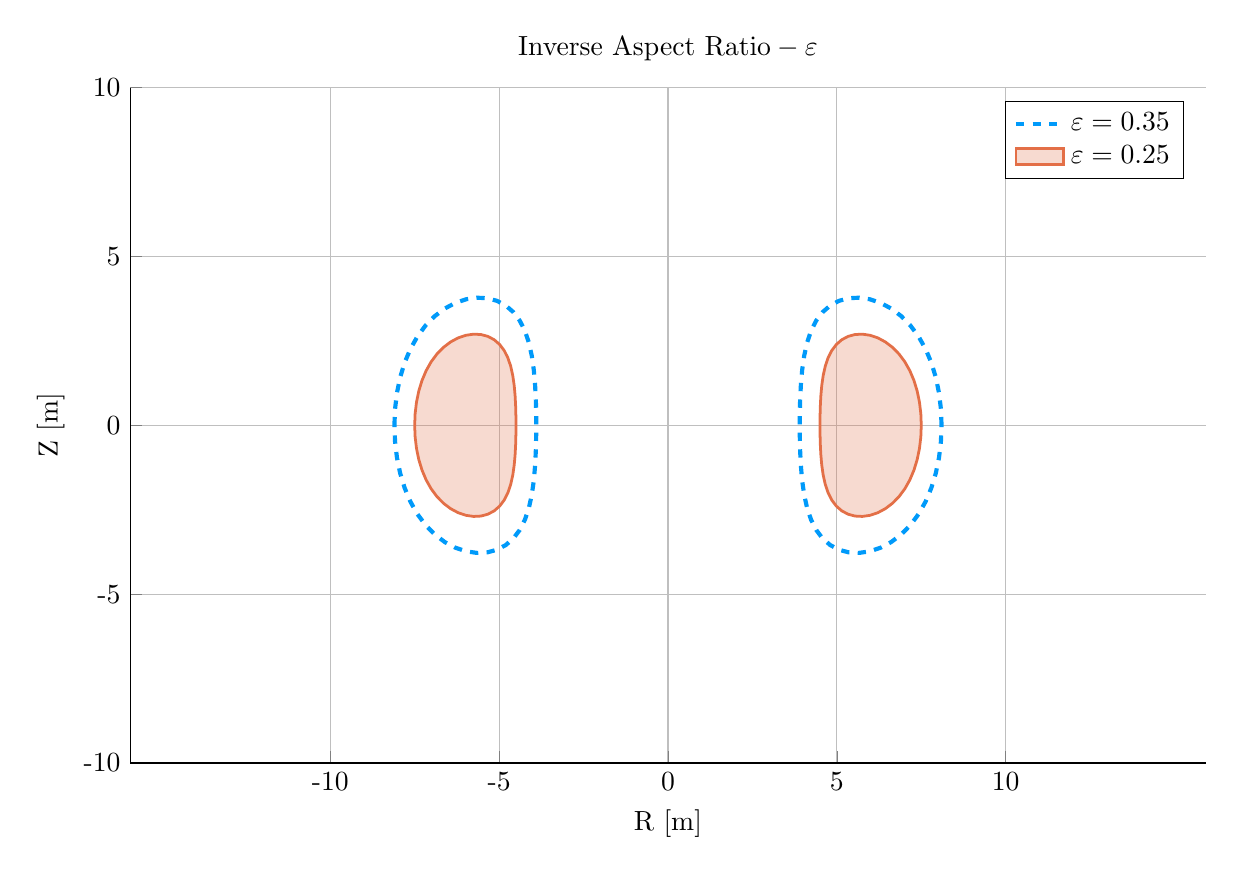
\begin{tikzpicture}[]
\begin{axis}[height = {101.6mm}, axis equal = {true}, ylabel = {Z [m]}, title = {$\textnormal{Inverse Aspect Ratio} - \varepsilon$}, xmin = {-10}, xmax = {10}, ymax = {10}, xlabel = {R [m]}, {unbounded coords=jump, scaled x ticks = false, xticklabel style={rotate = 0}, xmajorgrids = true, xtick = {-10.0,-5.0,0.0,5.0,10.0}, xticklabels = {-10,-5,0,5,10}, xtick align = inside, axis lines* = left, scaled y ticks = false, yticklabel style={rotate = 0}, ymajorgrids = true, ytick = {-10.0,-5.0,0.0,5.0,10.0}, yticklabels = {-10,-5,0,5,10}, ytick align = inside, axis lines* = left,     xshift = 0.0mm,
    yshift = 0.0mm,
    axis background/.style={fill={rgb,1:red,1.00000000;green,1.00000000;blue,1.00000000}}
}, ymin = {-10}, width = {152.4mm}]\addplot+ [color = {rgb,1:red,0.00000000;green,0.60560316;blue,0.97868012},
draw opacity=1.0,
line width=1.5,
dashed,mark = none,
mark size = 2.0,
mark options = {
    color = {rgb,1:red,0.00000000;green,0.00000000;blue,0.00000000}, draw opacity = 1.0,
    fill = {rgb,1:red,0.00000000;green,0.60560316;blue,0.97868012}, fill opacity = 1.0,
    line width = 1,
    rotate = 0,
    solid
}]coordinates {
(8.1, 0.0)
(8.081204069972497, 0.48337567116743263)
(8.024684777757766, 0.9588143271779377)
(7.930141280572084, 1.4185092784440338)
(7.797367695668915, 1.854912346574885)
(7.626640572703316, 2.260857805256796)
(7.419158721180681, 2.6296800412811785)
(7.177452352825953, 2.9553230037291525)
(6.905679431512412, 3.232439644160208)
(6.609741255084048, 3.456479714999771)
(6.297174663233395, 3.623764484478577)
(5.976811190071814, 3.7315471413066206)
(5.658229090447864, 3.7780578972385994)
(5.351057127458824, 3.7625330469479685)
(5.06421429716898, 3.685227508047293)
(4.805183334632925, 3.547410635348094)
(4.579415603765742, 3.3513453780899396)
(4.389950548568067, 3.100251122376493)
(4.237306076467235, 2.7982508289446923)
(4.119660690046763, 2.45030333426344)
(4.033308834588962, 2.0621219265758737)
(3.9733333500050683, 1.6400805338643698)
(3.9344084806536994, 1.1911090641292867)
(3.911628010194501, 0.7225796164911881)
(3.9012485454184915, 0.24218543152709598)
(3.9012485454184915, -0.2421854315270951)
(3.911628010194501, -0.7225796164911872)
(3.9344084806536994, -1.1911090641292859)
(3.9733333500050687, -1.640080533864369)
(4.033308834588962, -2.0621219265758732)
(4.119660690046763, -2.450303334263439)
(4.237306076467235, -2.7982508289446915)
(4.389950548568066, -3.1002511223764917)
(4.579415603765742, -3.3513453780899396)
(4.8051833346329245, -3.5474106353480934)
(5.064214297168979, -3.685227508047293)
(5.351057127458825, -3.7625330469479685)
(5.658229090447862, -3.7780578972385994)
(5.976811190071814, -3.731547141306621)
(6.297174663233394, -3.6237644844785772)
(6.609741255084048, -3.456479714999771)
(6.90567943151241, -3.232439644160209)
(7.177452352825952, -2.955323003729153)
(7.419158721180681, -2.629680041281178)
(7.626640572703316, -2.260857805256797)
(7.797367695668915, -1.854912346574885)
(7.930141280572083, -1.4185092784440358)
(8.024684777757766, -0.9588143271779382)
(8.081204069972497, -0.483375671167435)
(8.1, -9.258329801553988e-16)
};
\addlegendentry{$\varepsilon = 0.35$}
\addplot+ [color = {rgb,1:red,0.00000000;green,0.60560316;blue,0.97868012},
draw opacity=1.0,
line width=1.5,
dashed,mark = none,
mark size = 2.0,
mark options = {
    color = {rgb,1:red,0.00000000;green,0.00000000;blue,0.00000000}, draw opacity = 1.0,
    fill = {rgb,1:red,0.00000000;green,0.60560316;blue,0.97868012}, fill opacity = 1.0,
    line width = 1,
    rotate = 0,
    solid
},forget plot]coordinates {
(-8.1, 0.0)
(-8.081204069972497, 0.48337567116743263)
(-8.024684777757766, 0.9588143271779377)
(-7.930141280572084, 1.4185092784440338)
(-7.797367695668915, 1.854912346574885)
(-7.626640572703316, 2.260857805256796)
(-7.419158721180681, 2.6296800412811785)
(-7.177452352825953, 2.9553230037291525)
(-6.905679431512412, 3.232439644160208)
(-6.609741255084048, 3.456479714999771)
(-6.297174663233395, 3.623764484478577)
(-5.976811190071814, 3.7315471413066206)
(-5.658229090447864, 3.7780578972385994)
(-5.351057127458824, 3.7625330469479685)
(-5.06421429716898, 3.685227508047293)
(-4.805183334632925, 3.547410635348094)
(-4.579415603765742, 3.3513453780899396)
(-4.389950548568067, 3.100251122376493)
(-4.237306076467235, 2.7982508289446923)
(-4.119660690046763, 2.45030333426344)
(-4.033308834588962, 2.0621219265758737)
(-3.9733333500050683, 1.6400805338643698)
(-3.9344084806536994, 1.1911090641292867)
(-3.911628010194501, 0.7225796164911881)
(-3.9012485454184915, 0.24218543152709598)
(-3.9012485454184915, -0.2421854315270951)
(-3.911628010194501, -0.7225796164911872)
(-3.9344084806536994, -1.1911090641292859)
(-3.9733333500050687, -1.640080533864369)
(-4.033308834588962, -2.0621219265758732)
(-4.119660690046763, -2.450303334263439)
(-4.237306076467235, -2.7982508289446915)
(-4.389950548568066, -3.1002511223764917)
(-4.579415603765742, -3.3513453780899396)
(-4.8051833346329245, -3.5474106353480934)
(-5.064214297168979, -3.685227508047293)
(-5.351057127458825, -3.7625330469479685)
(-5.658229090447862, -3.7780578972385994)
(-5.976811190071814, -3.731547141306621)
(-6.297174663233394, -3.6237644844785772)
(-6.609741255084048, -3.456479714999771)
(-6.90567943151241, -3.232439644160209)
(-7.177452352825952, -2.955323003729153)
(-7.419158721180681, -2.629680041281178)
(-7.626640572703316, -2.260857805256797)
(-7.797367695668915, -1.854912346574885)
(-7.930141280572083, -1.4185092784440358)
(-8.024684777757766, -0.9588143271779382)
(-8.081204069972497, -0.483375671167435)
(-8.1, -9.258329801553988e-16)
};
\addplot+ [color = {rgb,1:red,0.88887350;green,0.43564919;blue,0.27812294},
draw opacity=1.0,
line width=1,
solid,mark = none,
mark size = 2.0,
mark options = {
    color = {rgb,1:red,0.00000000;green,0.00000000;blue,0.00000000}, draw opacity = 1.0,
    fill = {rgb,1:red,0.88887350;green,0.43564919;blue,0.27812294}, fill opacity = 1.0,
    line width = 1,
    rotate = 0,
    solid
},fill = {rgb,1:red,0.88887350;green,0.43564919;blue,0.27812294}, fill opacity=0.25,area legend]coordinates {
(7.5, 0.0)
(7.486574335694641, 0.34526833654816624)
(7.446203412684119, 0.6848673765556699)
(7.378672343265774, 1.0132209131743102)
(7.283834068334939, 1.3249373904106323)
(7.161886123359512, 1.6148984323262832)
(7.013684800843344, 1.8783428866294134)
(6.841037394875681, 2.1109450026636805)
(6.646913879651723, 2.3088854601144346)
(6.435529467917177, 2.468914082142694)
(6.212267616595282, 2.588403203198984)
(5.98343656433701, 2.6653908152190153)
(5.755877921748474, 2.6986127837418574)
(5.536469376756303, 2.687523604962835)
(5.331581640834985, 2.632305362890924)
(5.146559524737804, 2.533864739534353)
(4.985296859832673, 2.3938181272071004)
(4.84996467754862, 2.214465087411781)
(4.74093291176231, 1.998750592103352)
(4.6569004928905455, 1.7502166673310287)
(4.595220596134973, 1.4729442332684815)
(4.552380964289334, 1.1714860956174071)
(4.524577486181213, 0.8507921886637764)
(4.508305721567501, 0.5161282974937058)
(4.500891818156065, 0.17298959394792573)
(4.500891818156065, -0.1729895939479251)
(4.508305721567501, -0.5161282974937051)
(4.524577486181213, -0.8507921886637757)
(4.552380964289334, -1.1714860956174067)
(4.595220596134973, -1.472944233268481)
(4.656900492890545, -1.7502166673310282)
(4.74093291176231, -1.9987505921033515)
(4.849964677548619, -2.21446508741178)
(4.985296859832673, -2.3938181272071004)
(5.146559524737803, -2.5338647395343528)
(5.331581640834985, -2.632305362890924)
(5.536469376756303, -2.687523604962835)
(5.755877921748473, -2.6986127837418574)
(5.98343656433701, -2.6653908152190153)
(6.212267616595281, -2.5884032031989843)
(6.435529467917177, -2.468914082142694)
(6.646913879651722, -2.3088854601144355)
(6.841037394875681, -2.110945002663681)
(7.013684800843344, -1.878342886629413)
(7.161886123359511, -1.6148984323262838)
(7.283834068334939, -1.3249373904106323)
(7.378672343265773, -1.0132209131743115)
(7.446203412684119, -0.6848673765556703)
(7.486574335694641, -0.3452683365481679)
(7.5, -6.613092715395707e-16)
};
\addlegendentry{$\varepsilon = 0.25$}
\addplot+ [color = {rgb,1:red,0.88887350;green,0.43564919;blue,0.27812294},
draw opacity=1.0,
line width=1,
solid,mark = none,
mark size = 2.0,
mark options = {
    color = {rgb,1:red,0.00000000;green,0.00000000;blue,0.00000000}, draw opacity = 1.0,
    fill = {rgb,1:red,0.88887350;green,0.43564919;blue,0.27812294}, fill opacity = 1.0,
    line width = 1,
    rotate = 0,
    solid
},fill = {rgb,1:red,0.88887350;green,0.43564919;blue,0.27812294}, fill opacity=0.25,forget plot]coordinates {
(-7.5, 0.0)
(-7.486574335694641, 0.34526833654816624)
(-7.446203412684119, 0.6848673765556699)
(-7.378672343265774, 1.0132209131743102)
(-7.283834068334939, 1.3249373904106323)
(-7.161886123359512, 1.6148984323262832)
(-7.013684800843344, 1.8783428866294134)
(-6.841037394875681, 2.1109450026636805)
(-6.646913879651723, 2.3088854601144346)
(-6.435529467917177, 2.468914082142694)
(-6.212267616595282, 2.588403203198984)
(-5.98343656433701, 2.6653908152190153)
(-5.755877921748474, 2.6986127837418574)
(-5.536469376756303, 2.687523604962835)
(-5.331581640834985, 2.632305362890924)
(-5.146559524737804, 2.533864739534353)
(-4.985296859832673, 2.3938181272071004)
(-4.84996467754862, 2.214465087411781)
(-4.74093291176231, 1.998750592103352)
(-4.6569004928905455, 1.7502166673310287)
(-4.595220596134973, 1.4729442332684815)
(-4.552380964289334, 1.1714860956174071)
(-4.524577486181213, 0.8507921886637764)
(-4.508305721567501, 0.5161282974937058)
(-4.500891818156065, 0.17298959394792573)
(-4.500891818156065, -0.1729895939479251)
(-4.508305721567501, -0.5161282974937051)
(-4.524577486181213, -0.8507921886637757)
(-4.552380964289334, -1.1714860956174067)
(-4.595220596134973, -1.472944233268481)
(-4.656900492890545, -1.7502166673310282)
(-4.74093291176231, -1.9987505921033515)
(-4.849964677548619, -2.21446508741178)
(-4.985296859832673, -2.3938181272071004)
(-5.146559524737803, -2.5338647395343528)
(-5.331581640834985, -2.632305362890924)
(-5.536469376756303, -2.687523604962835)
(-5.755877921748473, -2.6986127837418574)
(-5.98343656433701, -2.6653908152190153)
(-6.212267616595281, -2.5884032031989843)
(-6.435529467917177, -2.468914082142694)
(-6.646913879651722, -2.3088854601144355)
(-6.841037394875681, -2.110945002663681)
(-7.013684800843344, -1.878342886629413)
(-7.161886123359511, -1.6148984323262838)
(-7.283834068334939, -1.3249373904106323)
(-7.378672343265773, -1.0132209131743115)
(-7.446203412684119, -0.6848673765556703)
(-7.486574335694641, -0.3452683365481679)
(-7.5, -6.613092715395707e-16)
};
\end{axis}

\end{tikzpicture}

		\end{adjustbox}
        \caption{$\epsilon$}
    \end{subfigure} ~\\ ~\\
    \caption{Geometric Parameters} ~\\
    \small These three geometric parameters allow the toroidal cross-sections to scale radially, stretch vertically, and become more triangular -- improving upon simple circular slices.
    \label{fig:geometry}
\end{figure*}

These geometric factors allow the volumetric and surface integrals for current, density, and temperature to be condensed to simple radial ones -- see \cref{eq:qs,eq:qv}. The only remaining step is to define the radial profiles for these three plasma quantities.

\subsection{Prescribing Plasma Profiles}

The first step in defining radial profiles is realizing that all three quantities are basically parabolas -- i.e. the temperature, density, and current are peaked at some radius (usually the center) and then decay to zero somewhere before the walls of the tokamak enclosure.

\begin{figure*}
	\label{fig:profiles}
    \centering
    \hfill 
    \begin{subfigure}[t]{0.45\textwidth}
        \centering
		\begin{adjustbox}{width=\textwidth}
			\Large
			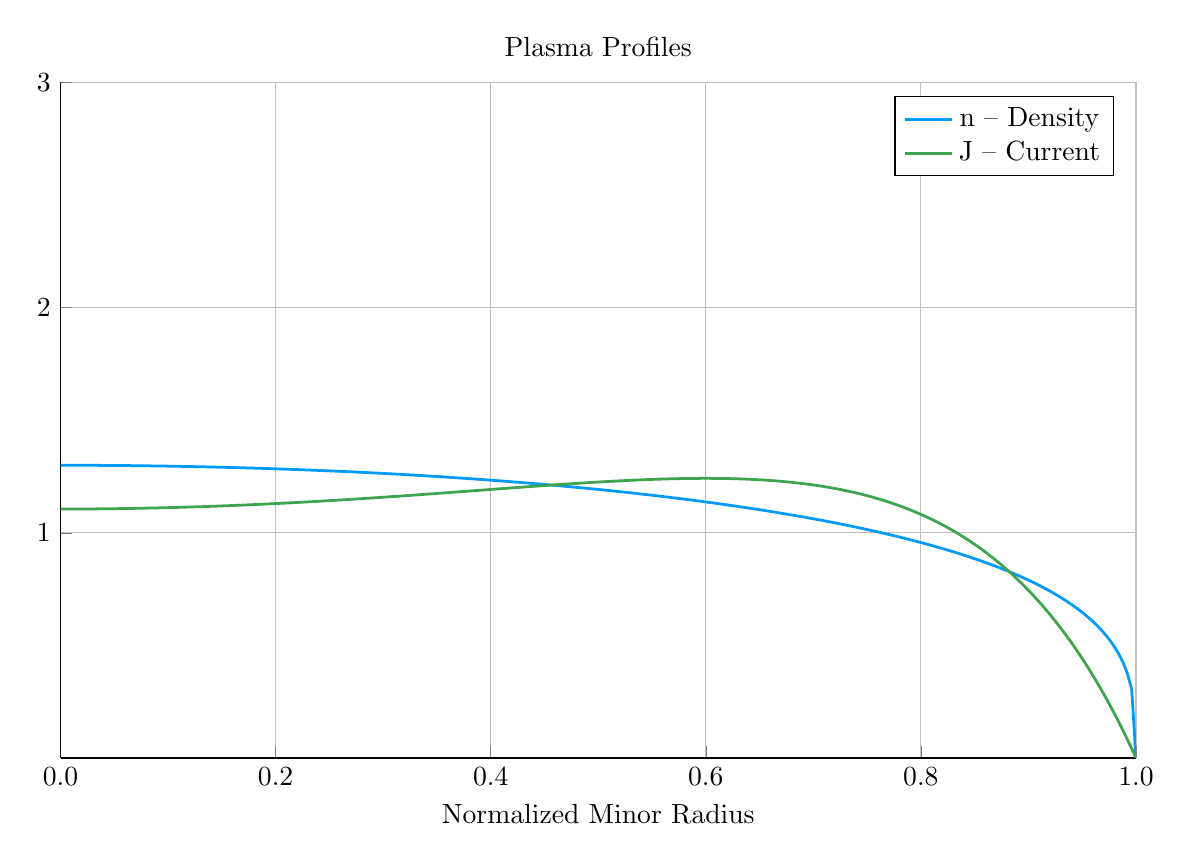
\begin{tikzpicture}[]
\begin{axis}[height = {101.6mm}, ylabel = {}, title = {Plasma Profiles}, xmin = {0.0}, xmax = {1.0}, ymax = {3}, xlabel = {Normalized Minor Radius}, {unbounded coords=jump, scaled x ticks = false, xticklabel style={rotate = 0}, xmajorgrids = true, xtick = {0.0,0.2,0.4,0.6000000000000001,0.8,1.0}, xticklabels = {0.0,0.2,0.4,0.6,0.8,1.0}, xtick align = inside, axis lines* = left, scaled y ticks = false, yticklabel style={rotate = 0}, ymajorgrids = true, ytick = {1.0,2.0,3.0}, yticklabels = {1,2,3}, ytick align = inside, axis lines* = left,     xshift = 0.0mm,
    yshift = 0.0mm,
    axis background/.style={fill={rgb,1:red,1.00000000;green,1.00000000;blue,1.00000000}}
}, ymin = {0}, width = {152.4mm}]\addplot+ [color = {rgb,1:red,0.00000000;green,0.60560316;blue,0.97868012},
draw opacity=1.0,
line width=1,
solid,mark = none,
mark size = 2.0,
mark options = {
    color = {rgb,1:red,0.00000000;green,0.00000000;blue,0.00000000}, draw opacity = 1.0,
    fill = {rgb,1:red,0.00000000;green,0.60560316;blue,0.97868012}, fill opacity = 1.0,
    line width = 1,
    rotate = 0,
    solid
}]coordinates {
(0.0, 1.3)
(0.004, 1.2999937599650557)
(0.008, 1.2999750394408758)
(0.012, 1.299943837169305)
(0.016, 1.2999001510530381)
(0.02, 1.2998439781550484)
(0.024, 1.2997753146977886)
(0.028, 1.2996941560621622)
(0.032, 1.2996004967862647)
(0.036, 1.2994943305638946)
(0.04, 1.2993756502428317)
(0.044, 1.2992444478228855)
(0.048, 1.2991007144537061)
(0.052, 1.2989444404323625)
(0.056, 1.2987756152006849)
(0.06, 1.2985942273423656)
(0.064, 1.2984002645798236)
(0.068, 1.2981937137708253)
(0.072, 1.2979745609048603)
(0.076, 1.2977427910992743)
(0.08, 1.2974983885951488)
(0.084, 1.2972413367529347)
(0.088, 1.2969716180478277)
(0.092, 1.2966892140648891)
(0.096, 1.2963941054939072)
(0.1, 1.2960862721239934)
(0.104, 1.2957656928379149)
(0.108, 1.2954323456061552)
(0.112, 1.295086207480701)
(0.116, 1.2947272545885533)
(0.12, 1.2943554621249538)
(0.124, 1.2939708043463278)
(0.128, 1.2935732545629344)
(0.132, 1.2931627851312222)
(0.136, 1.2927393674458851)
(0.14, 1.2923029719316104)
(0.144, 1.2918535680345185)
(0.148, 1.2913911242132843)
(0.152, 1.290915607929936)
(0.156, 1.2904269856403272)
(0.16, 1.2899252227842701)
(0.164, 1.289410283775332)
(0.168, 1.2888821319902795)
(0.172, 1.2883407297581677)
(0.176, 1.2877860383490682)
(0.18, 1.2872180179624235)
(0.184, 1.286636627715024)
(0.188, 1.286041825628597)
(0.192, 1.2854335686170009)
(0.196, 1.2848118124730112)
(0.2, 1.2841765118546966)
(0.204, 1.2835276202713661)
(0.208, 1.2828650900690854)
(0.212, 1.2821888724157464)
(0.216, 1.2814989172856817)
(0.22, 1.2807951734438123)
(0.224, 1.280077588429316)
(0.228, 1.2793461085388045)
(0.232, 1.2786006788089976)
(0.236, 1.2778412429988808)
(0.24, 1.2770677435713307)
(0.244, 1.2762801216741988)
(0.248, 1.275478317120833)
(0.252, 1.274662268370027)
(0.256, 1.2738319125053779)
(0.26, 1.2729871852140369)
(0.264, 1.2721280207648382)
(0.268, 1.2712543519857844)
(0.272, 1.2703661102408716)
(0.276, 1.2694632254062383)
(0.28, 1.268545625845612)
(0.284, 1.2676132383850391)
(0.288, 1.266665988286872)
(0.292, 1.2657037992229945)
(0.296, 1.2647265932472596)
(0.3, 1.2637342907671185)
(0.304, 1.262726810514414)
(0.308, 1.261704069515311)
(0.312, 1.2606659830593416)
(0.316, 1.2596124646675324)
(0.32, 1.2585434260595858)
(0.324, 1.257458777120088)
(0.328, 1.256358425863706)
(0.332, 1.2552422783993482)
(0.336, 1.2541102388932475)
(0.34, 1.2529622095309358)
(0.344, 1.2517980904780717)
(0.348, 1.2506177798400802)
(0.352, 1.24942117362057)
(0.356, 1.248208165678479)
(0.36, 1.2469786476839106)
(0.364, 1.2457325090726121)
(0.368, 1.2444696369990487)
(0.372, 1.2431899162880222)
(0.376, 1.2418932293847857)
(0.38, 1.2405794563035972)
(0.384, 1.239248474574658)
(0.388, 1.237900159189375)
(0.392, 1.2365343825438908)
(0.396, 1.2351510143808089)
(0.4, 1.2337499217290562)
(0.404, 1.2323309688418065)
(0.408, 1.2308940171323957)
(0.412, 1.229438925108151)
(0.416, 1.2279655483020526)
(0.42, 1.2264737392021483)
(0.424, 1.2249633471786308)
(0.428, 1.2234342184084848)
(0.432, 1.221886195797614)
(0.436, 1.2203191189003393)
(0.44, 1.2187328238361723)
(0.444, 1.2171271432037454)
(0.448, 1.2155019059917886)
(0.452, 1.2138569374870312)
(0.456, 1.212192059178898)
(0.46, 1.210507088660872)
(0.464, 1.208801839528379)
(0.468, 1.2070761212730492)
(0.472, 1.205329739173201)
(0.476, 1.2035624941803869)
(0.48, 1.2017741828018271)
(0.484, 1.1999645969785544)
(0.488, 1.1981335239590802)
(0.492, 1.1962807461683858)
(0.496, 1.1944060410720247)
(0.5, 1.1925091810351223)
(0.504, 1.190589933176035)
(0.508, 1.1886480592144295)
(0.512, 1.1866833153135188)
(0.516, 1.1846954519161883)
(0.52, 1.1826842135747218)
(0.524, 1.1806493387738237)
(0.528, 1.1785905597466213)
(0.532, 1.1765076022833005)
(0.536, 1.1744001855320279)
(0.54, 1.1722680217917714)
(0.544, 1.1701108162966227)
(0.548, 1.1679282669911981)
(0.552, 1.1657200642966656)
(0.556, 1.1634858908669246)
(0.56, 1.1612254213344295)
(0.564, 1.1589383220451273)
(0.568, 1.1566242507819302)
(0.572, 1.154282856476133)
(0.576, 1.1519137789061165)
(0.58, 1.1495166483826693)
(0.584, 1.1470910854201908)
(0.588, 1.1446367003930078)
(0.592, 1.142153093175977)
(0.596, 1.1396398527684999)
(0.6, 1.1370965569010092)
(0.604, 1.1345227716229302)
(0.608, 1.1319180508710498)
(0.612, 1.1292819360171518)
(0.616, 1.1266139553937018)
(0.62, 1.123913623796276)
(0.624, 1.1211804419613376)
(0.628, 1.1184138960178658)
(0.632, 1.1156134569112315)
(0.636, 1.1127785797976015)
(0.64, 1.1099087034070205)
(0.644, 1.1070032493731854)
(0.648, 1.1040616215277776)
(0.652, 1.1010832051570543)
(0.656, 1.0980673662182174)
(0.66, 1.0950134505129014)
(0.664, 1.0919207828148862)
(0.668, 1.0887886659489356)
(0.672, 1.0856163798173906)
(0.676, 1.082403180370883)
(0.68, 1.0791482985192302)
(0.684, 1.075850938978235)
(0.688, 1.0725102790477619)
(0.692, 1.0691254673160542)
(0.696, 1.0656956222848162)
(0.7, 1.0622198309091082)
(0.704, 1.0586971470455604)
(0.708, 1.055126589801824)
(0.712, 1.0515071417795323)
(0.716, 1.04783774720231)
(0.72, 1.0441173099195802)
(0.724, 1.0403446912760228)
(0.728, 1.03651870783555)
(0.732, 1.0326381289475657)
(0.736, 1.0287016741420443)
(0.74, 1.0247080103385948)
(0.744, 1.0206557488531367)
(0.748, 1.0165434421840995)
(0.752, 1.0123695805581145)
(0.756, 1.0081325882130072)
(0.76, 1.003830819393436)
(0.764, 0.9994625540317649)
(0.768, 0.9950259930836299)
(0.772, 0.990519253484107)
(0.776, 0.9859403626863661)
(0.78, 0.9812872527401133)
(0.784, 0.9765577538618856)
(0.788, 0.9717495874432898)
(0.792, 0.9668603584364187)
(0.796, 0.9618875470478029)
(0.8, 0.9568284996631833)
(0.804, 0.9516804189149115)
(0.808, 0.946440352791649)
(0.812, 0.9411051826759365)
(0.816, 0.9356716101787849)
(0.82, 0.9301361426212457)
(0.824, 0.9244950769904182)
(0.828, 0.9187444821708816)
(0.832, 0.9128801792212949)
(0.836, 0.9068977194288869)
(0.84, 0.900792359830521)
(0.844, 0.8945590358364464)
(0.848, 0.8881923305297794)
(0.852, 0.8816864401388146)
(0.856, 0.8750351350873486)
(0.86, 0.8682317159164477)
(0.864, 0.86126896323448)
(0.868, 0.8541390806843802)
(0.872, 0.8468336297096526)
(0.876, 0.8393434546426821)
(0.88, 0.8316585963161566)
(0.884, 0.8237681919917861)
(0.888, 0.81566035888456)
(0.892, 0.8073220579010558)
(0.896, 0.7987389333598728)
(0.9, 0.7898951233563103)
(0.904, 0.7807730339816926)
(0.908, 0.7713530686829113)
(0.912, 0.7616133014678136)
(0.916, 0.7515290791633757)
(0.92, 0.7410725331284098)
(0.924, 0.7302119741312908)
(0.928, 0.7189111346441375)
(0.932, 0.7071282092103691)
(0.936, 0.6948146236457978)
(0.94, 0.6819134341198397)
(0.944, 0.6683572117823803)
(0.948, 0.654065197526229)
(0.952, 0.6389393969490827)
(0.956, 0.6228590949732707)
(0.96, 0.6056729403361176)
(0.964, 0.5871871562979527)
(0.968, 0.5671473067124922)
(0.972, 0.5452087722509604)
(0.976, 0.520886146278826)
(0.98, 0.4934599473688843)
(0.984, 0.46178715390262587)
(0.988, 0.4238602013900372)
(0.992, 0.3755408186191309)
(0.996, 0.3052175562338072)
(1.0, 0.0)
};
\addlegendentry{n -- Density}
\addplot+ [color = {rgb,1:red,0.24222430;green,0.64327509;blue,0.30444865},
draw opacity=1.0,
line width=1,
solid,mark = none,
mark size = 2.0,
mark options = {
    color = {rgb,1:red,0.00000000;green,0.00000000;blue,0.00000000}, draw opacity = 1.0,
    fill = {rgb,1:red,0.24222430;green,0.64327509;blue,0.30444865}, fill opacity = 1.0,
    line width = 1,
    rotate = 0,
    solid
}]coordinates {
(0.0, 1.1055925931810484)
(0.004, 1.1056025434176453)
(0.008, 1.105632392966404)
(0.012, 1.1056821383432776)
(0.016, 1.1057517737383413)
(0.02, 1.1058412910110205)
(0.024, 1.1059506796834087)
(0.028, 1.106079926931665)
(0.032, 1.106229017575493)
(0.036, 1.1063979340656915)
(0.04, 1.106586656469768)
(0.044, 1.1067951624556105)
(0.048, 1.107023427273207)
(0.052, 1.1072714237343937)
(0.056, 1.1075391221906397)
(0.06, 1.107826490508826)
(0.064, 1.1081334940450354)
(0.068, 1.1084600956163122)
(0.072, 1.1088062554703932)
(0.076, 1.1091719312533783)
(0.08, 1.1095570779753314)
(0.084, 1.1099616479737875)
(0.088, 1.110385590875139)
(0.092, 1.1108288535538926)
(0.096, 1.1112913800897515)
(0.1, 1.1117731117225211)
(0.104, 1.1122739868047913)
(0.108, 1.112793940752376)
(0.112, 1.1133329059924844)
(0.116, 1.1138908119095834)
(0.12, 1.1144675847889256)
(0.124, 1.115063147757707)
(0.128, 1.1156774207238216)
(0.132, 1.1163103203121705)
(0.136, 1.1169617597984949)
(0.14, 1.1176316490406888)
(0.144, 1.11831989440755)
(0.148, 1.119026398704931)
(0.152, 1.11975106109924)
(0.156, 1.120493777038251)
(0.16, 1.1212544381691738)
(0.164, 1.1220329322539315)
(0.168, 1.1228291430816038)
(0.172, 1.1236429503779706)
(0.176, 1.1244742297121144)
(0.18, 1.1253228524000167)
(0.184, 1.1261886854050946)
(0.188, 1.127071591235615)
(0.192, 1.1279714278389303)
(0.196, 1.128888048492462)
(0.2, 1.1298213016913794)
(0.204, 1.1307710310328927)
(0.208, 1.131737075097102)
(0.212, 1.1327192673243216)
(0.216, 1.1337174358888118)
(0.22, 1.1347314035688367)
(0.224, 1.135760987612975)
(0.228, 1.136805999602598)
(0.232, 1.1378662453104351)
(0.236, 1.1389415245551366)
(0.24, 1.140031631051753)
(0.244, 1.1411363522580324)
(0.248, 1.1422554692164475)
(0.252, 1.143388756391854)
(0.256, 1.1445359815046836)
(0.26, 1.145696905359567)
(0.264, 1.146871281669287)
(0.268, 1.1480588568739498)
(0.272, 1.1492593699552682)
(0.276, 1.1504725522458386)
(0.28, 1.1516981272333027)
(0.284, 1.1529358103592642)
(0.288, 1.1541853088128475)
(0.292, 1.1554463213187653)
(0.296, 1.1567185379197655)
(0.3, 1.15800163975333)
(0.304, 1.1592952988224805)
(0.308, 1.160599177760553)
(0.312, 1.1619129295898027)
(0.316, 1.1632361974736778)
(0.32, 1.1645686144626213)
(0.324, 1.1659098032332398)
(0.328, 1.1672593758206753)
(0.332, 1.1686169333440195)
(0.336, 1.1699820657245965)
(0.34, 1.171354351396943)
(0.344, 1.1727333570123062)
(0.348, 1.1741186371344703)
(0.352, 1.1755097339277303)
(0.356, 1.176906176836817)
(0.36, 1.1783074822585666)
(0.364, 1.1797131532051435)
(0.368, 1.181122678958593)
(0.372, 1.1825355347165192)
(0.376, 1.1839511812286583)
(0.38, 1.1853690644241248)
(0.384, 1.1867886150290958)
(0.388, 1.1882092481746926)
(0.392, 1.1896303629948166)
(0.396, 1.1910513422136817)
(0.4, 1.1924715517227884)
(0.404, 1.1938903401470713)
(0.408, 1.1953070383999467)
(0.412, 1.1967209592269779)
(0.416, 1.198131396737873)
(0.42, 1.199537625926516)
(0.424, 1.2009389021787291)
(0.428, 1.2023344607674524)
(0.432, 1.2037235163350242)
(0.436, 1.205105262362225)
(0.44, 1.2064788706237588)
(0.444, 1.2078434906298132)
(0.448, 1.2091982490533475)
(0.452, 1.2105422491427469)
(0.456, 1.2118745701194584)
(0.46, 1.2131942665602276)
(0.464, 1.2145003677635429)
(0.468, 1.2157918770998737)
(0.472, 1.2170677713452926)
(0.476, 1.218326999998044)
(0.48, 1.219568484577629)
(0.484, 1.220791117905943)
(0.488, 1.2219937633700142)
(0.492, 1.2231752541658545)
(0.496, 1.2243343925229389)
(0.5, 1.2254699489088112)
(0.504, 1.2265806612132972)
(0.508, 1.227665233911794)
(0.512, 1.2287223372070952)
(0.516, 1.229750606149186)
(0.52, 1.2307486397324405)
(0.524, 1.2317149999696246)
(0.528, 1.2326482109421029)
(0.532, 1.2335467578256245)
(0.536, 1.234409085891052)
(0.54, 1.235233599479366)
(0.544, 1.2360186609502908)
(0.548, 1.2367625896038223)
(0.552, 1.2374636605739702)
(0.556, 1.2381201036939686)
(0.56, 1.2387301023322053)
(0.564, 1.2392917921981084)
(0.568, 1.2398032601171822)
(0.572, 1.2402625427743916)
(0.576, 1.2406676254250506)
(0.58, 1.241016440572357)
(0.584, 1.2413068666106932)
(0.588, 1.2415367264337844)
(0.592, 1.2417037860067774)
(0.596, 1.2418057529012922)
(0.6, 1.2418402747924557)
(0.604, 1.2418049379169072)
(0.608, 1.2416972654907381)
(0.612, 1.2415147160863034)
(0.616, 1.2412546819667964)
(0.62, 1.2409144873774753)
(0.624, 1.24049138679237)
(0.628, 1.2399825631152874)
(0.632, 1.239385125833895)
(0.636, 1.2386961091256128)
(0.64, 1.2379124699140391)
(0.644, 1.2370310858745734)
(0.648, 1.2360487533878732)
(0.652, 1.2349621854397481)
(0.656, 1.233768009466043)
(0.66, 1.2324627651410391)
(0.664, 1.2310429021078442)
(0.668, 1.2295047776492094)
(0.672, 1.2278446542971666)
(0.676, 1.2260586973798364)
(0.68, 1.224142972503699)
(0.684, 1.2220934429695933)
(0.688, 1.219905967120643)
(0.692, 1.2175762956202625)
(0.696, 1.2151000686583564)
(0.7, 1.2124728130837497)
(0.704, 1.2096899394608527)
(0.708, 1.206746739048499)
(0.712, 1.2036383806988336)
(0.716, 1.200359907674078)
(0.72, 1.1969062343789294)
(0.724, 1.1932721430062943)
(0.728, 1.1894522800939817)
(0.732, 1.1854411529899347)
(0.736, 1.181233126223481)
(0.74, 1.1768224177800433)
(0.744, 1.172203095276651)
(0.748, 1.1673690720355396)
(0.752, 1.162314103053033)
(0.756, 1.1570317808608346)
(0.76, 1.1515155312767646)
(0.764, 1.1457586090418983)
(0.768, 1.1397540933409778)
(0.772, 1.133494883202872)
(0.776, 1.1269736927777798)
(0.78, 1.1201830464877607)
(0.784, 1.1131152740470984)
(0.788, 1.1057625053488873)
(0.792, 1.0981166652141365)
(0.796, 1.0901694679995795)
(0.8, 1.0819124120602648)
(0.804, 1.0733367740628939)
(0.808, 1.064433603145756)
(0.812, 1.0551937149209845)
(0.816, 1.0456076853147525)
(0.82, 1.0356658442408755)
(0.824, 1.0253582691031793)
(0.828, 1.0146747781218477)
(0.832, 1.0036049234788245)
(0.836, 0.99213798427721)
(0.84, 0.980262959309437)
(0.844, 0.9679685596288679)
(0.848, 0.9552432009192925)
(0.852, 0.9420749956566505)
(0.856, 0.9284517450571373)
(0.86, 0.9143609308056804)
(0.864, 0.8997897065585966)
(0.868, 0.8847248892140719)
(0.872, 0.8691529499438978)
(0.876, 0.8530600049797328)
(0.88, 0.8364318061469402)
(0.884, 0.819253731138866)
(0.888, 0.8015107735241939)
(0.892, 0.783187532479819)
(0.896, 0.7642682022414483)
(0.9, 0.7447365612639053)
(0.904, 0.72457596108289)
(0.908, 0.7037693148696959)
(0.912, 0.6822990856701381)
(0.916, 0.6601472743186879)
(0.92, 0.6372954070185461)
(0.924, 0.6137245225781115)
(0.928, 0.5894151592940192)
(0.932, 0.564347341470635)
(0.936, 0.5385005655655922)
(0.94, 0.5118537859506463)
(0.944, 0.48438540027680593)
(0.948, 0.45607323443237957)
(0.952, 0.4268945270822218)
(0.956, 0.39682591377612964)
(0.96, 0.3658434106139833)
(0.964, 0.3339223974548356)
(0.968, 0.30103760065679763)
(0.972, 0.2671630753341644)
(0.976, 0.23227218711781)
(0.98, 0.19633759340448617)
(0.984, 0.15933122408020503)
(0.988, 0.12122426170246466)
(0.992, 0.08198712112559489)
(0.996, 0.04158942855305283)
(1.0, 0.0)
};
\addlegendentry{J -- Current}
\end{axis}

\end{tikzpicture}

		\end{adjustbox}
        \caption{Density and Current Profiles}
    \end{subfigure}
    \hfill
    \begin{subfigure}[t]{0.45\textwidth}
        \centering
		\begin{adjustbox}{width=\textwidth}
			\Large
			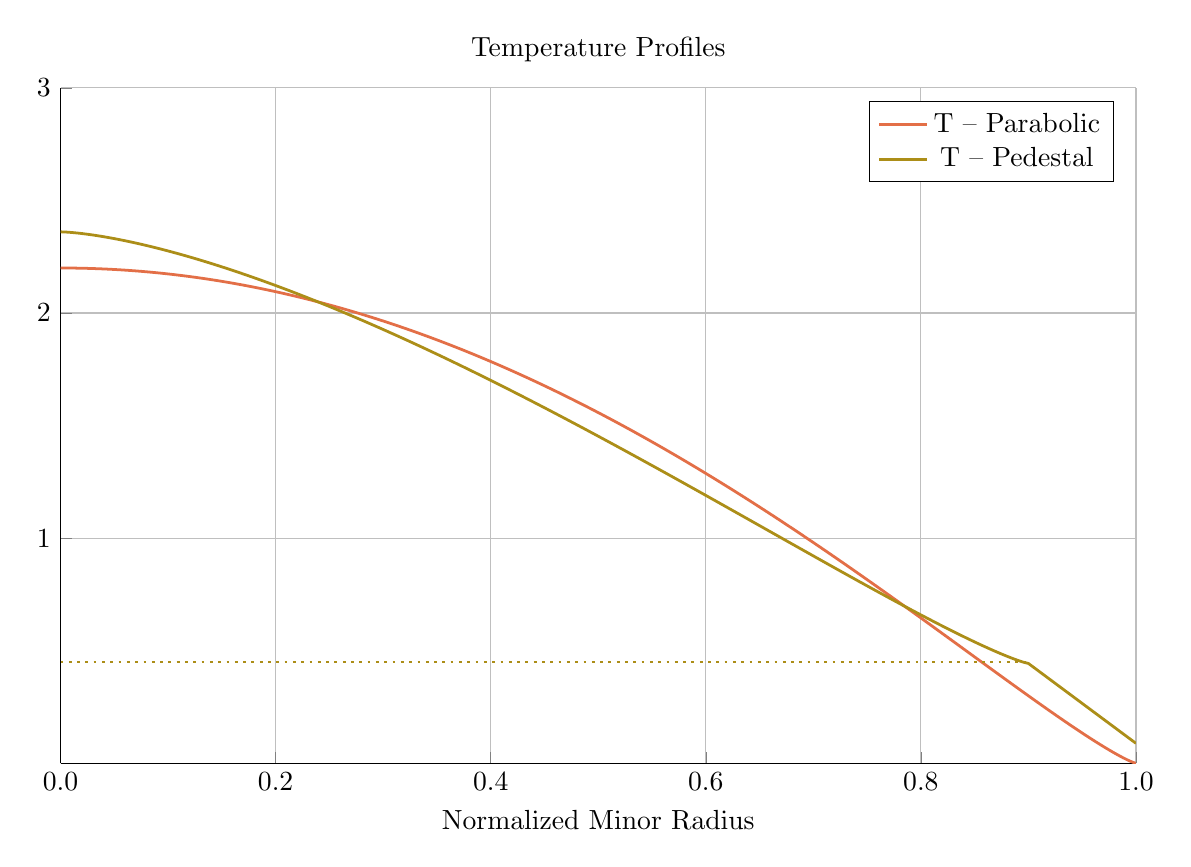
\begin{tikzpicture}[]
\begin{axis}[height = {101.6mm}, ylabel = {}, title = {Temperature Profiles}, xmin = {0.0}, xmax = {1.0}, ymax = {3}, xlabel = {Normalized Minor Radius}, {unbounded coords=jump, scaled x ticks = false, xticklabel style={rotate = 0}, xmajorgrids = true, xtick = {0.0,0.2,0.4,0.6000000000000001,0.8,1.0}, xticklabels = {0.0,0.2,0.4,0.6,0.8,1.0}, xtick align = inside, axis lines* = left, scaled y ticks = false, yticklabel style={rotate = 0}, ymajorgrids = true, ytick = {1.0,2.0,3.0}, yticklabels = {1,2,3}, ytick align = inside, axis lines* = left,     xshift = 0.0mm,
    yshift = 0.0mm,
    axis background/.style={fill={rgb,1:red,1.00000000;green,1.00000000;blue,1.00000000}}
}, ymin = {0}, width = {152.4mm}]\addplot+ [color = {rgb,1:red,0.88887350;green,0.43564919;blue,0.27812294},
draw opacity=1.0,
line width=1,
solid,mark = none,
mark size = 2.0,
mark options = {
    color = {rgb,1:red,0.00000000;green,0.00000000;blue,0.00000000}, draw opacity = 1.0,
    fill = {rgb,1:red,0.88887350;green,0.43564919;blue,0.27812294}, fill opacity = 1.0,
    line width = 1,
    rotate = 0,
    solid
}]coordinates {
(0.0, 2.2)
(0.004, 2.1999577600675844)
(0.008, 2.199831041081363)
(0.012, 2.199619845474514)
(0.016, 2.1993241773026853)
(0.02, 2.198944042244507)
(0.024, 2.1984794476023213)
(0.028, 2.1979304023031214)
(0.032, 2.1972969168996905)
(0.036, 2.196579003571959)
(0.04, 2.195776676128566)
(0.044, 2.194889950008634)
(0.048, 2.1939188422837517)
(0.052, 2.192863371660171)
(0.056, 2.1917235584812182)
(0.06, 2.1904994247299143)
(0.064, 2.189190994031813)
(0.068, 2.187798291658056)
(0.072, 2.1863213445286407)
(0.076, 2.1847601812159145)
(0.08, 2.1831148319482794)
(0.084, 2.1813853286141245)
(0.088, 2.179571704765981)
(0.092, 2.1776739956248985)
(0.096, 2.1756922380850554)
(0.1, 2.1736264707185855)
(0.104, 2.1714767337806498)
(0.108, 2.1692430692147298)
(0.112, 2.1669255206581606)
(0.116, 2.164524133447901)
(0.12, 2.1620389546265417)
(0.124, 2.1594700329485588)
(0.128, 2.1568174188868077)
(0.132, 2.154081164639269)
(0.136, 2.1512613241360428)
(0.14, 2.148357953046596)
(0.144, 2.1453711087872693)
(0.148, 2.1423008505290397)
(0.152, 2.139147239205551)
(0.156, 2.1359103375214086)
(0.16, 2.1325902099607443)
(0.164, 2.129186922796058)
(0.168, 2.1257005440973358)
(0.172, 2.1221311437414503)
(0.176, 2.1184787934218474)
(0.18, 2.1147435666585284)
(0.184, 2.1109255388083183)
(0.188, 2.1070247870754453)
(0.192, 2.1030413905224172)
(0.196, 2.098975430081212)
(0.2, 2.09482698856478)
(0.204, 2.090596150678874)
(0.208, 2.086283003034196)
(0.212, 2.0818876341588837)
(0.216, 2.0774101345113314)
(0.22, 2.072850596493357)
(0.224, 2.068209114463716)
(0.228, 2.063485784751976)
(0.232, 2.058680705672756)
(0.236, 2.053793977540332)
(0.24, 2.0488257026836245)
(0.244, 2.043775985461571)
(0.248, 2.038644932278893)
(0.252, 2.033432651602259)
(0.256, 2.0281392539768675)
(0.26, 2.022764852043437)
(0.264, 2.0173095605556335)
(0.268, 2.0117734963979244)
(0.272, 2.006156778603888)
(0.276, 2.0004595283749724)
(0.28, 1.9946818690997206)
(0.284, 1.9888239263734737)
(0.288, 1.9828858280185606)
(0.292, 1.976867704104986)
(0.296, 1.9707696869716258)
(0.3, 1.9645919112479475)
(0.304, 1.9583345138762616)
(0.308, 1.9519976341345224)
(0.312, 1.9455814136596863)
(0.316, 1.939085996471644)
(0.32, 1.932511528997742)
(0.324, 1.9258581600979061)
(0.328, 1.9191260410903783)
(0.332, 1.912315325778094)
(0.336, 1.9054261704757012)
(0.34, 1.8984587340372499)
(0.344, 1.8914131778845642)
(0.348, 1.8842896660363146)
(0.352, 1.8770883651378103)
(0.356, 1.8698094444915332)
(0.36, 1.8624530760884261)
(0.364, 1.8550194346399664)
(0.368, 1.8475086976110369)
(0.372, 1.839921045253621)
(0.376, 1.8322566606413475)
(0.38, 1.8245157297049002)
(0.384, 1.8166984412683274)
(0.388, 1.8088049870862715)
(0.392, 1.8008355618821434)
(0.396, 1.792790363387276)
(0.4, 1.7846695923810785)
(0.404, 1.776473452732227)
(0.408, 1.7682021514409176)
(0.412, 1.7598558986822177)
(0.416, 1.7514349078505493)
(0.42, 1.742939395605332)
(0.424, 1.7343695819178346)
(0.428, 1.725725690119258)
(0.432, 1.7170079469501018)
(0.436, 1.7082165826108464)
(0.44, 1.6993518308139948)
(0.444, 1.6904139288375197)
(0.448, 1.6814031175797635)
(0.452, 1.6723196416158315)
(0.456, 1.6631637492555364)
(0.46, 1.653935692602939)
(0.464, 1.6446357276175452)
(0.468, 1.6352641141772097)
(0.472, 1.6258211161428078)
(0.476, 1.6163070014247378)
(0.48, 1.606722042051314)
(0.484, 1.5970665142391203)
(0.488, 1.5873406984653924)
(0.492, 1.5775448795424998)
(0.496, 1.5676793466946068)
(0.5, 1.5577443936365882)
(0.504, 1.5477403186552856)
(0.508, 1.5376674246931867)
(0.512, 1.5275260194346267)
(0.516, 1.517316415394591)
(0.52, 1.5070389300102414)
(0.524, 1.4966938857352434)
(0.528, 1.4862816101370295)
(0.532, 1.4758024359970894)
(0.536, 1.465256701414425)
(0.54, 1.4546447499122863)
(0.544, 1.4439669305483216)
(0.548, 1.4332235980282817)
(0.552, 1.4224151128234246)
(0.556, 1.4115418412917677)
(0.56, 1.4006041558033582)
(0.564, 1.3896024348697198)
(0.568, 1.3785370632776597)
(0.572, 1.3674084322276236)
(0.576, 1.3562169394767907)
(0.58, 1.3449629894871216)
(0.584, 1.333646993578575)
(0.588, 1.3222693700877242)
(0.592, 1.3108305445320172)
(0.596, 1.2993309497799401)
(0.6, 1.2877710262273512)
(0.604, 1.2761512219802742)
(0.608, 1.2644719930444575)
(0.612, 1.2527338035220144)
(0.616, 1.2409371258154922)
(0.62, 1.2290824408397232)
(0.624, 1.2171702382418437)
(0.628, 1.2052010166298843)
(0.632, 1.1931752838103635)
(0.636, 1.1810935570353371)
(0.64, 1.1689563632593918)
(0.644, 1.156764239407098)
(0.648, 1.1445177326514693)
(0.652, 1.1322174007040144)
(0.656, 1.1198638121170017)
(0.66, 1.1074575465986056)
(0.664, 1.0949991953416336)
(0.668, 1.082489361366603)
(0.672, 1.0699286598799627)
(0.676, 1.0573177186483342)
(0.68, 1.044657178389695)
(0.684, 1.0319476931824922)
(0.688, 1.019189930893753)
(0.692, 1.0063845736273342)
(0.696, 0.9935323181935332)
(0.7, 0.980633876601379)
(0.704, 0.9676899765750238)
(0.708, 0.9547013620957563)
(0.712, 0.9416687939712927)
(0.716, 0.9285930504341149)
(0.72, 0.9154749277707805)
(0.724, 0.9023152409842818)
(0.728, 0.8891148244917015)
(0.732, 0.8758745328596077)
(0.736, 0.8625952415798288)
(0.74, 0.849277847888491)
(0.744, 0.8359232716314423)
(0.748, 0.822532456179475)
(0.752, 0.8091063693970627)
(0.756, 0.7956460046686752)
(0.76, 0.7821523819871128)
(0.764, 0.7686265491087244)
(0.768, 0.7550695827808527)
(0.772, 0.7414825900473649)
(0.776, 0.7278667096387308)
(0.78, 0.7142231134537544)
(0.784, 0.7005530081408239)
(0.788, 0.6868576367873601)
(0.792, 0.6731382807270975)
(0.796, 0.6593962614758839)
(0.8, 0.6456329428078906)
(0.804, 0.6318497329854856)
(0.808, 0.6180480871575735)
(0.812, 0.6042295099429783)
(0.816, 0.5903955582174578)
(0.82, 0.5765478441252689)
(0.824, 0.5626880383388612)
(0.828, 0.5488178735933505)
(0.832, 0.5349391485259877)
(0.836, 0.5210537318549578)
(0.84, 0.5071635669366619)
(0.844, 0.49327067674623953)
(0.848, 0.47937716933269775)
(0.852, 0.46548524380775297)
(0.856, 0.45159719693668826)
(0.86, 0.4377154304104124)
(0.864, 0.42384245889091393)
(0.868, 0.40998091893787963)
(0.872, 0.3961335789430169)
(0.876, 0.38230335022134865)
(0.88, 0.36849329943642983)
(0.884, 0.35470666257034567)
(0.888, 0.340946860691165)
(0.892, 0.3272175178224195)
(0.896, 0.31352248128407095)
(0.9, 0.2998658449561726)
(0.904, 0.28625197602028446)
(0.908, 0.2726855458667975)
(0.912, 0.25917156602852953)
(0.916, 0.24571543022609155)
(0.92, 0.23232296390814428)
(0.924, 0.21900048306792003)
(0.928, 0.20575486465742054)
(0.932, 0.1925936316637043)
(0.936, 0.17952505695042487)
(0.94, 0.16655829144594192)
(0.944, 0.15370352440467291)
(0.948, 0.14097218665156444)
(0.952, 0.12837721256189286)
(0.956, 0.11593338410667639)
(0.96, 0.10365779254585625)
(0.964, 0.09157047392306764)
(0.968, 0.07969531062880889)
(0.972, 0.06806135815914495)
(0.976, 0.056704888286093984)
(0.98, 0.04567272289384328)
(0.984, 0.035028106493367024)
(0.988, 0.024862215823612335)
(0.992, 0.0153206738078139)
(0.996, 0.0066847830139362754)
(1.0, 0.0)
};
\addlegendentry{T -- Parabolic}
\addplot+ [color = {rgb,1:red,0.67554396;green,0.55566233;blue,0.09423434},
draw opacity=1.0,
line width=1,
solid,mark = none,
mark size = 2.0,
mark options = {
    color = {rgb,1:red,0.00000000;green,0.00000000;blue,0.00000000}, draw opacity = 1.0,
    fill = {rgb,1:red,0.67554396;green,0.55566233;blue,0.09423434}, fill opacity = 1.0,
    line width = 1,
    rotate = 0,
    solid
}]coordinates {
(0.0, 2.3605919704710323)
(0.004, 2.359910398918797)
(0.008, 2.3586642994783618)
(0.012, 2.3570508613498493)
(0.016, 2.3551405297956594)
(0.02, 2.3529740696983454)
(0.024, 2.350579025743975)
(0.028, 2.3479756517769723)
(0.032, 2.3451796682823796)
(0.036, 2.342203747147281)
(0.04, 2.3390583928390996)
(0.044, 2.3357525032801973)
(0.048, 2.332293746279636)
(0.052, 2.328688822918463)
(0.056, 2.3249436581415552)
(0.06, 2.3210635425572748)
(0.064, 2.3170532404255844)
(0.068, 2.3129170735482543)
(0.072, 2.3086589875663335)
(0.076, 2.3042826051438894)
(0.08, 2.299791269197131)
(0.084, 2.295188078444673)
(0.088, 2.2904759169492626)
(0.092, 2.2856574788975115)
(0.096, 2.2807352895619175)
(0.1, 2.2757117231701707)
(0.104, 2.2705890182452353)
(0.108, 2.2653692908590712)
(0.112, 2.260054546151598)
(0.116, 2.2546466883966962)
(0.12, 2.2491475298430212)
(0.124, 2.243558798515241)
(0.128, 2.237882145128044)
(0.132, 2.2321191492388524)
(0.136, 2.2262713247439767)
(0.14, 2.220340124805883)
(0.144, 2.2143269462853388)
(0.148, 2.2082331337408316)
(0.152, 2.202059983048349)
(0.156, 2.1958087446868073)
(0.16, 2.189480626728042)
(0.164, 2.1830767975648464)
(0.168, 2.176598388406032)
(0.172, 2.1700464955636813)
(0.176, 2.163422182554496)
(0.18, 2.1567264820344176)
(0.184, 2.149960397583317)
(0.188, 2.14312490535454)
(0.192, 2.1362209556023704)
(0.196, 2.1292494740989305)
(0.2, 2.1222113634507807)
(0.204, 2.1151075043243255)
(0.208, 2.1079387565881396)
(0.212, 2.1007059603794906)
(0.216, 2.0934099371015487)
(0.22, 2.0860514903571366)
(0.224, 2.0786314068242686)
(0.228, 2.0711504570782133)
(0.232, 2.063609396364366)
(0.236, 2.0560089653257996)
(0.24, 2.0483498906890096)
(0.244, 2.040632885911039)
(0.248, 2.0328586517908898)
(0.252, 2.0250278770478602)
(0.256, 2.0171412388692334)
(0.26, 2.009199403429513)
(0.264, 2.00120302638324)
(0.268, 1.9931527533332325)
(0.272, 1.9850492202759686)
(0.276, 1.97689305402566)
(0.28, 1.9686848726184767)
(0.284, 1.9604252856982425)
(0.288, 1.9521148948848384)
(0.292, 1.9437542941264454)
(0.296, 1.9353440700366855)
(0.3, 1.9268848022176337)
(0.304, 1.9183770635696087)
(0.308, 1.9098214205885893)
(0.312, 1.9012184336520364)
(0.316, 1.8925686572938556)
(0.32, 1.883872640469185)
(0.324, 1.8751309268096423)
(0.328, 1.8663440548696335)
(0.332, 1.8575125583642822)
(0.336, 1.8486369663995004)
(0.34, 1.839717803694704)
(0.344, 1.8307555907986295)
(0.348, 1.8217508442986934)
(0.352, 1.812704077024307)
(0.356, 1.8036157982445404)
(0.36, 1.7944865138605)
(0.364, 1.7853167265927747)
(0.368, 1.776106936164285)
(0.372, 1.7668576394788444)
(0.376, 1.7575693307957496)
(0.38, 1.74824250190067)
(0.384, 1.7388776422731294)
(0.388, 1.7294752392508332)
(0.392, 1.7200357781911024)
(0.396, 1.7105597426296557)
(0.4, 1.7010476144369753)
(0.404, 1.6914998739724885)
(0.408, 1.6819170002367874)
(0.412, 1.6722994710220926)
(0.416, 1.6626477630611856)
(0.42, 1.6529623521750014)
(0.424, 1.6432437134190898)
(0.428, 1.633492321229143)
(0.432, 1.6237086495657764)
(0.436, 1.6138931720587668)
(0.44, 1.6040463621509233)
(0.444, 1.5941686932417938)
(0.448, 1.584260638831387)
(0.452, 1.5743226726641009)
(0.456, 1.5643552688730447)
(0.46, 1.5543589021249482)
(0.464, 1.544334047765842)
(0.468, 1.5342811819677138)
(0.472, 1.5242007818763206)
(0.476, 1.5140933257603746)
(0.48, 1.5039592931622903)
(0.484, 1.4937991650507099)
(0.488, 1.4836134239750187)
(0.492, 1.473402554222062)
(0.496, 1.4631670419753044)
(0.5, 1.4529073754766455)
(0.504, 1.4426240451911474)
(0.508, 1.4323175439749165)
(0.512, 1.4219883672464035)
(0.516, 1.4116370131613858)
(0.52, 1.4012639827919213)
(0.524, 1.3908697803095635)
(0.528, 1.3804549131731465)
(0.532, 1.3700198923214701)
(0.536, 1.359565232371216)
(0.54, 1.349091451820459)
(0.544, 1.3385990732581485)
(0.548, 1.328088623579961)
(0.552, 1.3175606342109392)
(0.556, 1.307015641335371)
(0.56, 1.2964541861343752)
(0.564, 1.2858768150316933)
(0.568, 1.2752840799482301)
(0.572, 1.2646765385659007)
(0.576, 1.2540547546013914)
(0.58, 1.2434192980904786)
(0.584, 1.2327707456835955)
(0.588, 1.222109680953382)
(0.592, 1.211436694715004)
(0.596, 1.200752385360086)
(0.6, 1.1900573592051713)
(0.604, 1.1793522308556705)
(0.608, 1.1686376235863563)
(0.612, 1.1579141697395272)
(0.616, 1.1471825111420575)
(0.62, 1.1364432995426441)
(0.624, 1.1256971970706737)
(0.628, 1.1149448767182386)
(0.632, 1.1041870228469695)
(0.636, 1.093424331721486)
(0.64, 1.0826575120714315)
(0.644, 1.0718872856842108)
(0.648, 1.061114388030769)
(0.652, 1.0503395689269308)
(0.656, 1.039563593233075)
(0.66, 1.0287872415951647)
(0.664, 1.0180113112304485)
(0.668, 1.0072366167614726)
(0.672, 0.9964639911023957)
(0.676, 0.9856942864020085)
(0.68, 0.9749283750483018)
(0.684, 0.9641671507399459)
(0.688, 0.9534115296306018)
(0.692, 0.9426624515526333)
(0.696, 0.9319208813275146)
(0.7, 0.9211878101710503)
(0.704, 0.9104642572024598)
(0.708, 0.8997512710674346)
(0.712, 0.8890499316865009)
(0.716, 0.8783613521413978)
(0.72, 0.8676866807137728)
(0.724, 0.8570271030923351)
(0.728, 0.8463838447667099)
(0.732, 0.8357581736286817)
(0.736, 0.8251514028043623)
(0.74, 0.8145648937441141)
(0.744, 0.8040000596009286)
(0.748, 0.7934583689324995)
(0.752, 0.7829413497675711)
(0.756, 0.7724505940834616)
(0.76, 0.7619877627491815)
(0.764, 0.7515545909975108)
(0.768, 0.741152894500166)
(0.772, 0.7307845761331225)
(0.776, 0.7204516335348546)
(0.78, 0.710156167579369)
(0.784, 0.6999003919093338)
(0.788, 0.6896866437035094)
(0.792, 0.6795173958885602)
(0.796, 0.6693952710502226)
(0.8, 0.6593230573553601)
(0.804, 0.6493037268683398)
(0.808, 0.6393404567373293)
(0.812, 0.6294366538454373)
(0.816, 0.6195959836776518)
(0.82, 0.6098224043609094)
(0.824, 0.6001202071108945)
(0.828, 0.5904940646939226)
(0.832, 0.58094909002811)
(0.836, 0.5714909077694643)
(0.84, 0.562125742755608)
(0.844, 0.5528605306710853)
(0.848, 0.5437030585117963)
(0.852, 0.5346621457948362)
(0.856, 0.5257478827341294)
(0.86, 0.516971950132737)
(0.864, 0.5083480600719166)
(0.868, 0.49989258164201933)
(0.872, 0.4916254625709785)
(0.876, 0.48357164972903754)
(0.88, 0.47576340897240366)
(0.884, 0.4682444150948954)
(0.888, 0.4610777748740693)
(0.892, 0.45436452608473005)
(0.896, 0.44830036952087016)
(0.9, 0.44361517600666117)
(0.904, 0.429419490374448)
(0.908, 0.41522380474223486)
(0.912, 0.4010281191100217)
(0.916, 0.38683243347780855)
(0.92, 0.3726367478455953)
(0.924, 0.3584410622133822)
(0.928, 0.34424537658116894)
(0.932, 0.3300496909489558)
(0.936, 0.3158540053167426)
(0.94, 0.30165831968452983)
(0.944, 0.28746263405231665)
(0.948, 0.27326694842010346)
(0.952, 0.2590712627878903)
(0.956, 0.24487557715567715)
(0.96, 0.23067989152346396)
(0.964, 0.21648420589125078)
(0.968, 0.2022885202590376)
(0.972, 0.18809283462682444)
(0.976, 0.17389714899461126)
(0.98, 0.1597014633623981)
(0.984, 0.14550577773018494)
(0.988, 0.13131009209797176)
(0.992, 0.11711440646575859)
(0.996, 0.1029187208335454)
(1.0, 0.08872303520133223)
};
\addlegendentry{T -- Pedestal}
\addplot+ [color = {rgb,1:red,0.67554396;green,0.55566233;blue,0.09423434},
draw opacity=1.0,
line width=1,
dotted,mark = none,
mark size = 2.0,
mark options = {
    color = {rgb,1:red,0.00000000;green,0.00000000;blue,0.00000000}, draw opacity = 1.0,
    fill = {rgb,1:red,0.67554396;green,0.55566233;blue,0.09423434}, fill opacity = 1.0,
    line width = 1,
    rotate = 0,
    solid
},forget plot]coordinates {
(0.0, 0.45)
(0.9, 0.45)
};
\end{axis}

\end{tikzpicture}

		\end{adjustbox}
        \caption{Temperature Profiles}
    \end{subfigure}
    \hfill \hfill ~\\ ~\\ ~\\
    \caption{Radial Plasma Profiles} ~\\
    \small The three most fundamental properties of a fusion plasma are its temperature, density, and current. These profiles allow the model to reduce from three dimensions to half of one.
\end{figure*}

\subsubsection{The Density Profile}

To begin, density has the simplest profile. This is because it is relatively flat, remaining near the average value -- $\overline n$ -- throughout the body of the plasma until quickly decaying to zero near the edge of the plasma. For this reason, a parabolic profile with a very low peaking factor -- $\nu_n$ -- is well suited.

\begin{equation}
	n(\rho) = \overline n \cdot ( 1 + \nu_n ) \, \cdot ( 1 - \rho ^ 2 ) ^ {\nu_n}
\end{equation}
\myequations{Density Profile -- $n$}

\subsubsection{The Temperature Profile}

The use of a parabolic profile for the plasma temperature is slightly more dubious. This is because H-Mode plasmas are actually highly peaked at the center, decaying to a non-zero pedestal temperature near the edge before finally dropping sharply to zero. This model chooses to forego the pedestal representation for a simple parabolic one -- although the pedestal approach is discussed in the Appendix. Analogous to the density, $\overline T$ is the average value and $\nu_T$ is the peaking parameter.

\begin{equation}
	T(\rho) = \overline T \cdot ( 1 + \nu_T ) \, \cdot ( 1 - \rho ^ 2 ) ^ {\nu_T}
\end{equation}
\myequations{Temperature Profile -- $T$}

\subsubsection{The Current Profile}

The plasma current is the third profile and cannot safely be represented by a simple parabola. This is because having an adequate bootstrap current relies heavily on a profile being peaked off-axis -- i.e. at some radius not at the center. This hollow profile can then be modeled with the commonly given plasma internal inductance ($l_i$).

Concretely, the current's hollow profile is described by:

\begin{equation}
	J(\rho) = \bar{J} \cdot \frac{ \gamma ^ 2 \cdot ( 1 - \rho ^ 2 ) \cdot e^{ \gamma \rho^2 } }{ e^\gamma - 1 - \gamma}
\end{equation}
\myequations{Current Profile -- $J$}

Where $\gamma$ can be numerically solved for from the plasma internal inductance using the following relations -- with $b_p$ representing the normalized poloidal magnetic field.

\begin{equation}
	l_i = \frac{4 \kappa}{1+\kappa^2}	 \int_0^1 b_p^2 \ \frac{d\rho}{\rho}
\end{equation}
\myequations{Internal Inductance -- $l_i$}

\begin{equation}
	\label{eq:b_p}
	b_p(\rho) = \frac{ -e^{\gamma\rho^2} ( \gamma\rho^2 - 1 - \gamma ) - 1 - \gamma }{\rho \,( e^\gamma - 1 - \gamma ) }
\end{equation}
\myequations{Normalized Poloidal Magnetic Field -- $b_p$}

Combined, these three geometric parameters and profiles lay the foundation for this zero-dimensional fusion systems model.

\section{Solving the Steady Current}

As suggested, one of the most important equations in a fusion reactor is current balance. In steady-state operation, all of a plasma's current ($I_P$) must come from a combination of its own bootstrap current ($I_{BS}$), as well as auxiliary current drive ($I_{CD}$). This can be represented mathematically as:

\begin{equation}
	\label{eq:ibal}
	\tcboxmath{
	I_P = I_{BS} + I_{CD}
	}
\end{equation}
\myequations{Current Balance -- $I$}

The goal is then to write equations for bootstrap current and driven current. This will make heavy use of the Greenwald density limit. Without spoiling too much, the steady current is shown to be only a function of temperature! In other words, this current is independent of a tokamak's geometry and magnet strength. As will be pointed out then, though, a subtlety arises that will bring the two back into the picture -- self-consistency in the current drive efficiency ($\eta_{CD}$).

\subsection{Enforcing the Greenwald Density Limit}

The Greenwald density limit is ubiquitous in the field of fusion energy. It sets a hard limit on the density and how it scales with current and reactor size. Although currently lacking a true first-principles theoretical explanation, it does have true meaning in the design context. Operate at too low a density and run the risk of never entering H-Mode. Run the density too high, and cause the tokamak's plasma to disrupt catastrophically!\footnote{Even if a plasma exists in H-Mode and survives disruptions, working outside the Greenwaldian range almost always leads to degraded plasma transport -- which is bad.}

\begin{figure*}
    \centering
    \hfill 
    \begin{subfigure}[t]{0.45\textwidth}
        \centering
		\begin{adjustbox}{width=\textwidth}
			\Large
			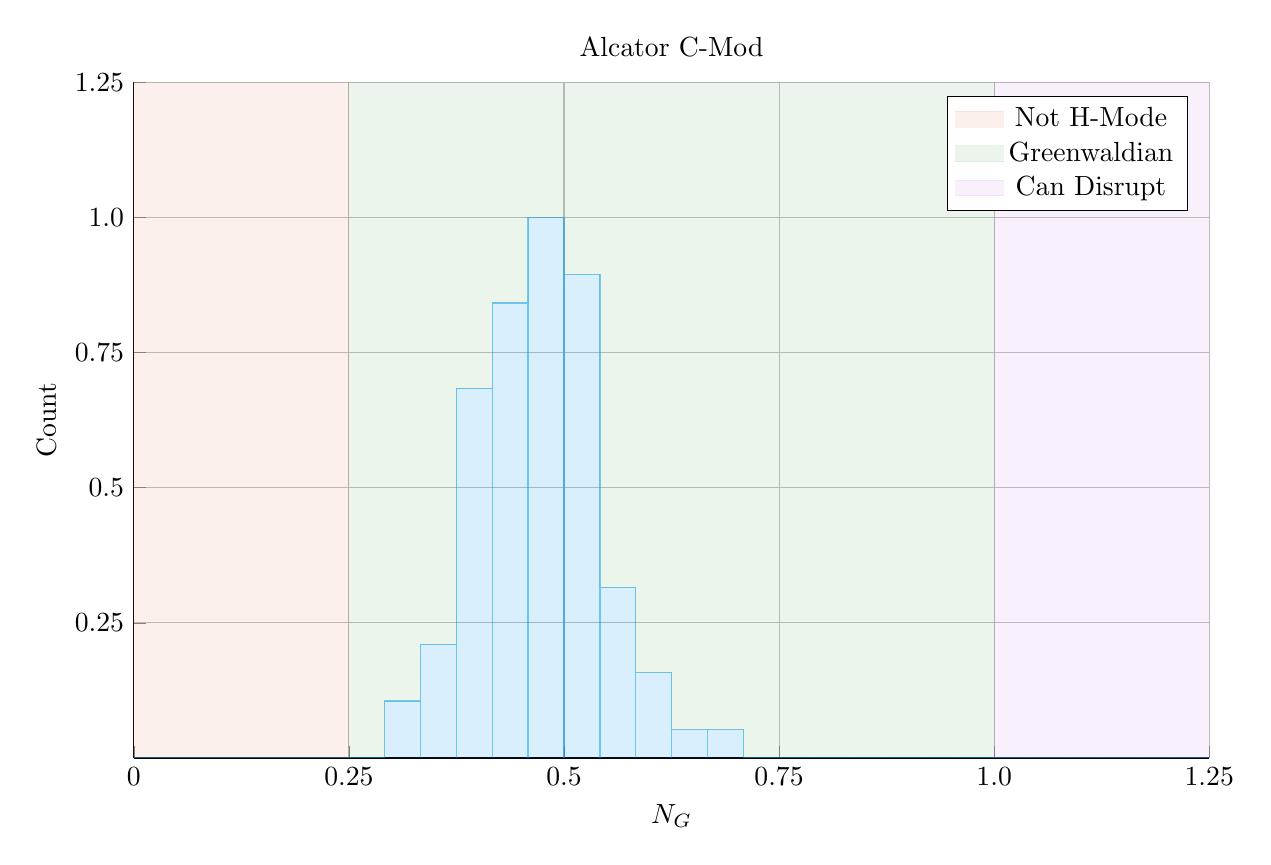
\begin{tikzpicture}[]
\begin{axis}[height = {101.6mm}, ylabel = {Count}, title = {Alcator C-Mod}, xmin = {0}, xmax = {1.25}, ymax = {1.25}, xlabel = {$N_G$}, {unbounded coords=jump, scaled x ticks = false, xticklabel style={rotate = 0}, xmajorgrids = true, xtick = {0.0,0.25,0.5,0.75,1.0,1.25}, xticklabels = {0,0.25,0.5,0.75,1.0,1.25}, xtick align = inside, axis lines* = left, scaled y ticks = false, yticklabel style={rotate = 0}, ymajorgrids = true, ytick = {0.0,0.25,0.5,0.75,1.0,1.25}, yticklabels = {,0.25,0.5,0.75,1.0,1.25}, ytick align = inside, axis lines* = left,     xshift = 0.0mm,
    yshift = 0.0mm,
    axis background/.style={fill={rgb,1:red,1.00000000;green,1.00000000;blue,1.00000000}}
}, ymin = {0}, width = {152.4mm}]\addplot+ [color = {rgb,1:red,0.00000000;green,0.60560316;blue,0.97868012},
draw opacity=0.5,
line width=0.5,
solid,mark = none,
mark size = 2.0,
mark options = {
    color = {rgb,1:red,0.00000000;green,0.00000000;blue,0.00000000}, draw opacity = 0.5,
    fill = {rgb,1:red,0.00000000;green,0.60560316;blue,0.97868012}, fill opacity = 0.5,
    line width = 1,
    rotate = 0,
    solid
},fill = {rgb,1:red,0.00000000;green,0.60560316;blue,0.97868012}, fill opacity=0.15,forget plot]coordinates {
(0.0, 0.0)
(0.0, 0.0)
(0.041666666666666664, 0.0)
(0.041666666666666664, 0.0)
(NaN, NaN)
(0.041666666666666664, 0.0)
(0.041666666666666664, 0.0)
(0.08333333333333333, 0.0)
(0.08333333333333333, 0.0)
(NaN, NaN)
(0.08333333333333333, 0.0)
(0.08333333333333333, 0.0)
(0.125, 0.0)
(0.125, 0.0)
(NaN, NaN)
(0.125, 0.0)
(0.125, 0.0)
(0.16666666666666666, 0.0)
(0.16666666666666666, 0.0)
(NaN, NaN)
(0.16666666666666666, 0.0)
(0.16666666666666666, 0.0)
(0.20833333333333334, 0.0)
(0.20833333333333334, 0.0)
(NaN, NaN)
(0.20833333333333334, 0.0)
(0.20833333333333334, 0.0)
(0.25, 0.0)
(0.25, 0.0)
(NaN, NaN)
(0.25, 0.0)
(0.25, 0.0)
(0.2916666666666667, 0.0)
(0.2916666666666667, 0.0)
(NaN, NaN)
(0.2916666666666667, 0.0)
(0.2916666666666667, 0.10526315789473684)
(0.3333333333333333, 0.10526315789473684)
(0.3333333333333333, 0.0)
(NaN, NaN)
(0.3333333333333333, 0.0)
(0.3333333333333333, 0.21052631578947367)
(0.375, 0.21052631578947367)
(0.375, 0.0)
(NaN, NaN)
(0.375, 0.0)
(0.375, 0.6842105263157895)
(0.4166666666666667, 0.6842105263157895)
(0.4166666666666667, 0.0)
(NaN, NaN)
(0.4166666666666667, 0.0)
(0.4166666666666667, 0.8421052631578947)
(0.4583333333333333, 0.8421052631578947)
(0.4583333333333333, 0.0)
(NaN, NaN)
(0.4583333333333333, 0.0)
(0.4583333333333333, 1.0)
(0.5, 1.0)
(0.5, 0.0)
(NaN, NaN)
(0.5, 0.0)
(0.5, 0.8947368421052632)
(0.5416666666666666, 0.8947368421052632)
(0.5416666666666666, 0.0)
(NaN, NaN)
(0.5416666666666666, 0.0)
(0.5416666666666666, 0.3157894736842105)
(0.5833333333333334, 0.3157894736842105)
(0.5833333333333334, 0.0)
(NaN, NaN)
(0.5833333333333334, 0.0)
(0.5833333333333334, 0.15789473684210525)
(0.625, 0.15789473684210525)
(0.625, 0.0)
(NaN, NaN)
(0.625, 0.0)
(0.625, 0.05263157894736842)
(0.6666666666666666, 0.05263157894736842)
(0.6666666666666666, 0.0)
(NaN, NaN)
(0.6666666666666666, 0.0)
(0.6666666666666666, 0.05263157894736842)
(0.7083333333333334, 0.05263157894736842)
(0.7083333333333334, 0.0)
(NaN, NaN)
(0.7083333333333334, 0.0)
(0.7083333333333334, 0.0)
(0.75, 0.0)
(0.75, 0.0)
(NaN, NaN)
(0.75, 0.0)
(0.75, 0.0)
(0.7916666666666666, 0.0)
(0.7916666666666666, 0.0)
(NaN, NaN)
(0.7916666666666666, 0.0)
(0.7916666666666666, 0.0)
(0.8333333333333334, 0.0)
(0.8333333333333334, 0.0)
(NaN, NaN)
(0.8333333333333334, 0.0)
(0.8333333333333334, 0.0)
(0.875, 0.0)
(0.875, 0.0)
(NaN, NaN)
(0.875, 0.0)
(0.875, 0.0)
(0.9166666666666666, 0.0)
(0.9166666666666666, 0.0)
(NaN, NaN)
(0.9166666666666666, 0.0)
(0.9166666666666666, 0.0)
(0.9583333333333334, 0.0)
(0.9583333333333334, 0.0)
(NaN, NaN)
(0.9583333333333334, 0.0)
(0.9583333333333334, 0.0)
(1.0, 0.0)
(1.0, 0.0)
(NaN, NaN)
(1.0, 0.0)
(1.0, 0.0)
(1.0416666666666667, 0.0)
(1.0416666666666667, 0.0)
(NaN, NaN)
(1.0416666666666667, 0.0)
(1.0416666666666667, 0.0)
(1.0833333333333333, 0.0)
(1.0833333333333333, 0.0)
(NaN, NaN)
(1.0833333333333333, 0.0)
(1.0833333333333333, 0.0)
(1.125, 0.0)
(1.125, 0.0)
(NaN, NaN)
(1.125, 0.0)
(1.125, 0.0)
(1.1666666666666667, 0.0)
(1.1666666666666667, 0.0)
(NaN, NaN)
(1.1666666666666667, 0.0)
(1.1666666666666667, 0.0)
(1.2083333333333333, 0.0)
(1.2083333333333333, 0.0)
(NaN, NaN)
(1.2083333333333333, 0.0)
(1.2083333333333333, 0.0)
(1.25, 0.0)
(1.25, 0.0)
(NaN, NaN)
};
\addplot+ [color = {rgb,1:red,0.88887350;green,0.43564919;blue,0.27812294},
draw opacity=0.1,
line width=0,
solid,mark = none,
mark size = 2.0,
mark options = {
    color = {rgb,1:red,0.00000000;green,0.00000000;blue,0.00000000}, draw opacity = 0.1,
    fill = {rgb,1:red,0.88887350;green,0.43564919;blue,0.27812294}, fill opacity = 0.1,
    line width = 1,
    rotate = 0,
    solid
},fill = {rgb,1:red,0.88887350;green,0.43564919;blue,0.27812294}, fill opacity=0.1,area legend]coordinates {
(0.0, 1.25)
(0.0, 0.0)
(0.041666666666666664, 0.0)
(0.041666666666666664, 0.0)
(0.08333333333333333, 0.0)
(0.08333333333333333, 0.0)
(0.125, 0.0)
(0.125, 0.0)
(0.16666666666666666, 0.0)
(0.16666666666666666, 0.0)
(0.20833333333333334, 0.0)
(0.20833333333333334, 0.0)
(0.25, 0.0)
(0.25, 1.25)
(0.0, 1.25)
};
\addlegendentry{Not H-Mode}
\addplot+ [color = {rgb,1:red,0.24222430;green,0.64327509;blue,0.30444865},
draw opacity=0.1,
line width=0,
solid,mark = none,
mark size = 2.0,
mark options = {
    color = {rgb,1:red,0.00000000;green,0.00000000;blue,0.00000000}, draw opacity = 0.1,
    fill = {rgb,1:red,0.24222430;green,0.64327509;blue,0.30444865}, fill opacity = 0.1,
    line width = 1,
    rotate = 0,
    solid
},fill = {rgb,1:red,0.24222430;green,0.64327509;blue,0.30444865}, fill opacity=0.1,area legend]coordinates {
(0.25, 1.25)
(0.25, 0.0)
(0.2916666666666667, 0.0)
(0.2916666666666667, 0.10526315789473684)
(0.3333333333333333, 0.10526315789473684)
(0.3333333333333333, 0.21052631578947367)
(0.375, 0.21052631578947367)
(0.375, 0.6842105263157895)
(0.4166666666666667, 0.6842105263157895)
(0.4166666666666667, 0.8421052631578947)
(0.4583333333333333, 0.8421052631578947)
(0.4583333333333333, 1.0)
(0.5, 1.0)
(0.5, 0.8947368421052632)
(0.5416666666666666, 0.8947368421052632)
(0.5416666666666666, 0.3157894736842105)
(0.5833333333333334, 0.3157894736842105)
(0.5833333333333334, 0.15789473684210525)
(0.625, 0.15789473684210525)
(0.625, 0.05263157894736842)
(0.6666666666666666, 0.05263157894736842)
(0.6666666666666666, 0.05263157894736842)
(0.7083333333333334, 0.05263157894736842)
(0.7083333333333334, 0.0)
(0.75, 0.0)
(0.75, 0.0)
(0.7916666666666666, 0.0)
(0.7916666666666666, 0.0)
(0.8333333333333334, 0.0)
(0.8333333333333334, 0.0)
(0.875, 0.0)
(0.875, 0.0)
(0.9166666666666666, 0.0)
(0.9166666666666666, 0.0)
(0.9583333333333334, 0.0)
(0.9583333333333334, 0.0)
(1.0, 0.0)
(1.0, 1.25)
(0.25, 1.25)
};
\addlegendentry{Greenwaldian}
\addplot+ [color = {rgb,1:red,0.76444018;green,0.44411178;blue,0.82429754},
draw opacity=0.1,
line width=0,
solid,mark = none,
mark size = 2.0,
mark options = {
    color = {rgb,1:red,0.00000000;green,0.00000000;blue,0.00000000}, draw opacity = 0.1,
    fill = {rgb,1:red,0.76444018;green,0.44411178;blue,0.82429754}, fill opacity = 0.1,
    line width = 1,
    rotate = 0,
    solid
},fill = {rgb,1:red,0.76444018;green,0.44411178;blue,0.82429754}, fill opacity=0.1,area legend]coordinates {
(1.0, 1.25)
(1.0, 0.0)
(1.0416666666666667, 0.0)
(1.0416666666666667, 0.0)
(1.0833333333333333, 0.0)
(1.0833333333333333, 0.0)
(1.125, 0.0)
(1.125, 0.0)
(1.1666666666666667, 0.0)
(1.1666666666666667, 0.0)
(1.2083333333333333, 0.0)
(1.2083333333333333, 0.0)
(1.25, 0.0)
(1.25, 1.25)
(1.0, 1.25)
};
\addlegendentry{Can Disrupt}
\end{axis}

\end{tikzpicture}

		\end{adjustbox}
        \caption{C-Mod}
    \end{subfigure}
    \hfill
    \begin{subfigure}[t]{0.45\textwidth}
        \centering
		\begin{adjustbox}{width=\textwidth}
			\Large
			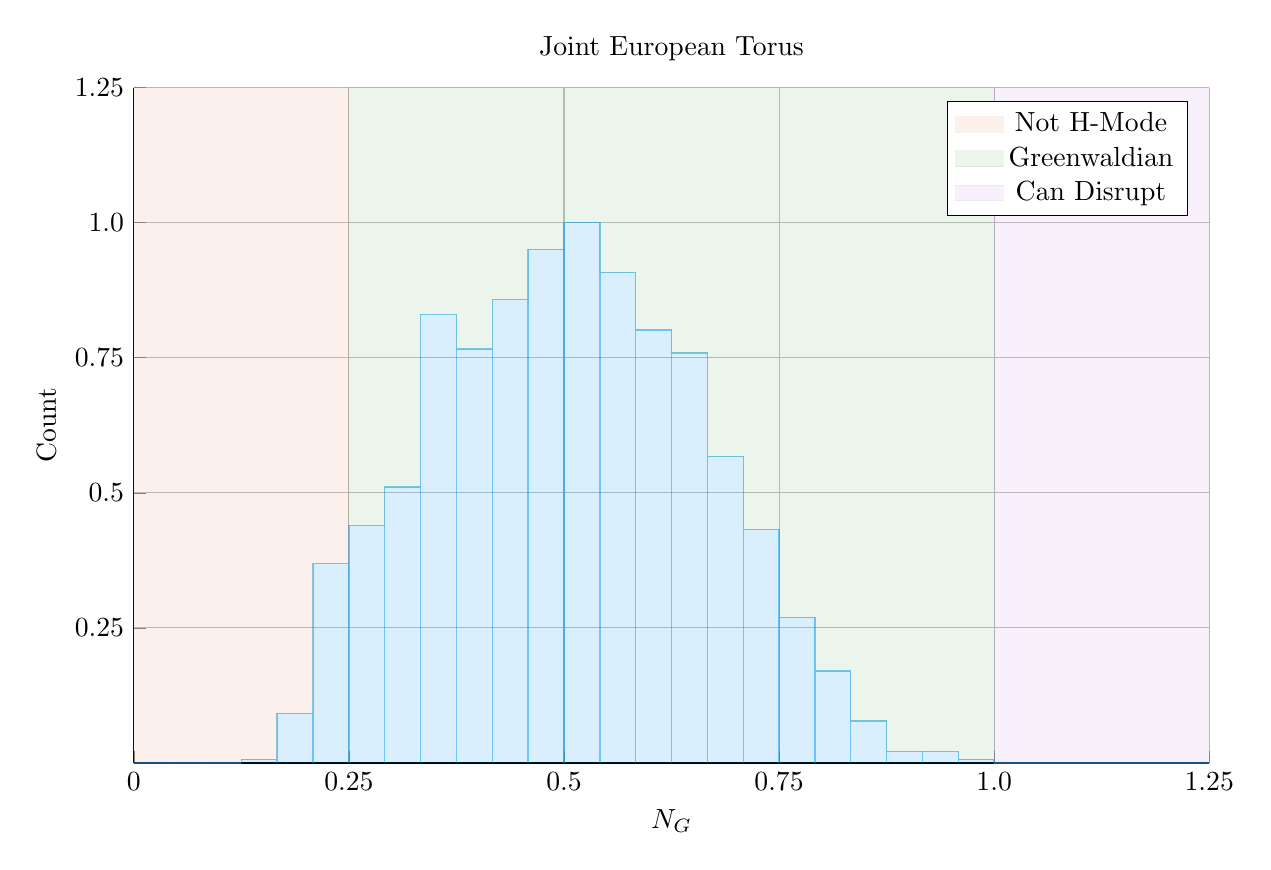
\begin{tikzpicture}[]
\begin{axis}[height = {101.6mm}, ylabel = {Count}, title = {Joint European Torus}, xmin = {0}, xmax = {1.25}, ymax = {1.25}, xlabel = {$N_G$}, {unbounded coords=jump, scaled x ticks = false, xticklabel style={rotate = 0}, xmajorgrids = true, xtick = {0.0,0.25,0.5,0.75,1.0,1.25}, xticklabels = {0,0.25,0.5,0.75,1.0,1.25}, xtick align = inside, axis lines* = left, scaled y ticks = false, yticklabel style={rotate = 0}, ymajorgrids = true, ytick = {0.0,0.25,0.5,0.75,1.0,1.25}, yticklabels = {,0.25,0.5,0.75,1.0,1.25}, ytick align = inside, axis lines* = left,     xshift = 0.0mm,
    yshift = 0.0mm,
    axis background/.style={fill={rgb,1:red,1.00000000;green,1.00000000;blue,1.00000000}}
}, ymin = {0}, width = {152.4mm}]\addplot+ [color = {rgb,1:red,0.00000000;green,0.60560316;blue,0.97868012},
draw opacity=0.5,
line width=0.5,
solid,mark = none,
mark size = 2.0,
mark options = {
    color = {rgb,1:red,0.00000000;green,0.00000000;blue,0.00000000}, draw opacity = 0.5,
    fill = {rgb,1:red,0.00000000;green,0.60560316;blue,0.97868012}, fill opacity = 0.5,
    line width = 1,
    rotate = 0,
    solid
},fill = {rgb,1:red,0.00000000;green,0.60560316;blue,0.97868012}, fill opacity=0.15,forget plot]coordinates {
(0.0, 0.0)
(0.0, 0.0)
(0.041666666666666664, 0.0)
(0.041666666666666664, 0.0)
(NaN, NaN)
(0.041666666666666664, 0.0)
(0.041666666666666664, 0.0)
(0.08333333333333333, 0.0)
(0.08333333333333333, 0.0)
(NaN, NaN)
(0.08333333333333333, 0.0)
(0.08333333333333333, 0.0)
(0.125, 0.0)
(0.125, 0.0)
(NaN, NaN)
(0.125, 0.0)
(0.125, 0.0070921985815602835)
(0.16666666666666666, 0.0070921985815602835)
(0.16666666666666666, 0.0)
(NaN, NaN)
(0.16666666666666666, 0.0)
(0.16666666666666666, 0.09219858156028368)
(0.20833333333333334, 0.09219858156028368)
(0.20833333333333334, 0.0)
(NaN, NaN)
(0.20833333333333334, 0.0)
(0.20833333333333334, 0.36879432624113473)
(0.25, 0.36879432624113473)
(0.25, 0.0)
(NaN, NaN)
(0.25, 0.0)
(0.25, 0.4397163120567376)
(0.2916666666666667, 0.4397163120567376)
(0.2916666666666667, 0.0)
(NaN, NaN)
(0.2916666666666667, 0.0)
(0.2916666666666667, 0.5106382978723404)
(0.3333333333333333, 0.5106382978723404)
(0.3333333333333333, 0.0)
(NaN, NaN)
(0.3333333333333333, 0.0)
(0.3333333333333333, 0.8297872340425532)
(0.375, 0.8297872340425532)
(0.375, 0.0)
(NaN, NaN)
(0.375, 0.0)
(0.375, 0.7659574468085106)
(0.4166666666666667, 0.7659574468085106)
(0.4166666666666667, 0.0)
(NaN, NaN)
(0.4166666666666667, 0.0)
(0.4166666666666667, 0.8581560283687943)
(0.4583333333333333, 0.8581560283687943)
(0.4583333333333333, 0.0)
(NaN, NaN)
(0.4583333333333333, 0.0)
(0.4583333333333333, 0.950354609929078)
(0.5, 0.950354609929078)
(0.5, 0.0)
(NaN, NaN)
(0.5, 0.0)
(0.5, 1.0)
(0.5416666666666666, 1.0)
(0.5416666666666666, 0.0)
(NaN, NaN)
(0.5416666666666666, 0.0)
(0.5416666666666666, 0.9078014184397163)
(0.5833333333333334, 0.9078014184397163)
(0.5833333333333334, 0.0)
(NaN, NaN)
(0.5833333333333334, 0.0)
(0.5833333333333334, 0.8014184397163121)
(0.625, 0.8014184397163121)
(0.625, 0.0)
(NaN, NaN)
(0.625, 0.0)
(0.625, 0.7588652482269503)
(0.6666666666666666, 0.7588652482269503)
(0.6666666666666666, 0.0)
(NaN, NaN)
(0.6666666666666666, 0.0)
(0.6666666666666666, 0.5673758865248227)
(0.7083333333333334, 0.5673758865248227)
(0.7083333333333334, 0.0)
(NaN, NaN)
(0.7083333333333334, 0.0)
(0.7083333333333334, 0.4326241134751773)
(0.75, 0.4326241134751773)
(0.75, 0.0)
(NaN, NaN)
(0.75, 0.0)
(0.75, 0.2695035460992908)
(0.7916666666666666, 0.2695035460992908)
(0.7916666666666666, 0.0)
(NaN, NaN)
(0.7916666666666666, 0.0)
(0.7916666666666666, 0.1702127659574468)
(0.8333333333333334, 0.1702127659574468)
(0.8333333333333334, 0.0)
(NaN, NaN)
(0.8333333333333334, 0.0)
(0.8333333333333334, 0.07801418439716312)
(0.875, 0.07801418439716312)
(0.875, 0.0)
(NaN, NaN)
(0.875, 0.0)
(0.875, 0.02127659574468085)
(0.9166666666666666, 0.02127659574468085)
(0.9166666666666666, 0.0)
(NaN, NaN)
(0.9166666666666666, 0.0)
(0.9166666666666666, 0.02127659574468085)
(0.9583333333333334, 0.02127659574468085)
(0.9583333333333334, 0.0)
(NaN, NaN)
(0.9583333333333334, 0.0)
(0.9583333333333334, 0.0070921985815602835)
(1.0, 0.0070921985815602835)
(1.0, 0.0)
(NaN, NaN)
(1.0, 0.0)
(1.0, 0.0)
(1.0416666666666667, 0.0)
(1.0416666666666667, 0.0)
(NaN, NaN)
(1.0416666666666667, 0.0)
(1.0416666666666667, 0.0)
(1.0833333333333333, 0.0)
(1.0833333333333333, 0.0)
(NaN, NaN)
(1.0833333333333333, 0.0)
(1.0833333333333333, 0.0)
(1.125, 0.0)
(1.125, 0.0)
(NaN, NaN)
(1.125, 0.0)
(1.125, 0.0)
(1.1666666666666667, 0.0)
(1.1666666666666667, 0.0)
(NaN, NaN)
(1.1666666666666667, 0.0)
(1.1666666666666667, 0.0)
(1.2083333333333333, 0.0)
(1.2083333333333333, 0.0)
(NaN, NaN)
(1.2083333333333333, 0.0)
(1.2083333333333333, 0.0)
(1.25, 0.0)
(1.25, 0.0)
(NaN, NaN)
};
\addplot+ [color = {rgb,1:red,0.88887350;green,0.43564919;blue,0.27812294},
draw opacity=0.1,
line width=0,
solid,mark = none,
mark size = 2.0,
mark options = {
    color = {rgb,1:red,0.00000000;green,0.00000000;blue,0.00000000}, draw opacity = 0.1,
    fill = {rgb,1:red,0.88887350;green,0.43564919;blue,0.27812294}, fill opacity = 0.1,
    line width = 1,
    rotate = 0,
    solid
},fill = {rgb,1:red,0.88887350;green,0.43564919;blue,0.27812294}, fill opacity=0.1,area legend]coordinates {
(0.0, 1.25)
(0.0, 0.0)
(0.041666666666666664, 0.0)
(0.041666666666666664, 0.0)
(0.08333333333333333, 0.0)
(0.08333333333333333, 0.0)
(0.125, 0.0)
(0.125, 0.0070921985815602835)
(0.16666666666666666, 0.0070921985815602835)
(0.16666666666666666, 0.09219858156028368)
(0.20833333333333334, 0.09219858156028368)
(0.20833333333333334, 0.36879432624113473)
(0.25, 0.36879432624113473)
(0.25, 1.25)
(0.0, 1.25)
};
\addlegendentry{Not H-Mode}
\addplot+ [color = {rgb,1:red,0.24222430;green,0.64327509;blue,0.30444865},
draw opacity=0.1,
line width=0,
solid,mark = none,
mark size = 2.0,
mark options = {
    color = {rgb,1:red,0.00000000;green,0.00000000;blue,0.00000000}, draw opacity = 0.1,
    fill = {rgb,1:red,0.24222430;green,0.64327509;blue,0.30444865}, fill opacity = 0.1,
    line width = 1,
    rotate = 0,
    solid
},fill = {rgb,1:red,0.24222430;green,0.64327509;blue,0.30444865}, fill opacity=0.1,area legend]coordinates {
(0.25, 1.25)
(0.25, 0.4397163120567376)
(0.2916666666666667, 0.4397163120567376)
(0.2916666666666667, 0.5106382978723404)
(0.3333333333333333, 0.5106382978723404)
(0.3333333333333333, 0.8297872340425532)
(0.375, 0.8297872340425532)
(0.375, 0.7659574468085106)
(0.4166666666666667, 0.7659574468085106)
(0.4166666666666667, 0.8581560283687943)
(0.4583333333333333, 0.8581560283687943)
(0.4583333333333333, 0.950354609929078)
(0.5, 0.950354609929078)
(0.5, 1.0)
(0.5416666666666666, 1.0)
(0.5416666666666666, 0.9078014184397163)
(0.5833333333333334, 0.9078014184397163)
(0.5833333333333334, 0.8014184397163121)
(0.625, 0.8014184397163121)
(0.625, 0.7588652482269503)
(0.6666666666666666, 0.7588652482269503)
(0.6666666666666666, 0.5673758865248227)
(0.7083333333333334, 0.5673758865248227)
(0.7083333333333334, 0.4326241134751773)
(0.75, 0.4326241134751773)
(0.75, 0.2695035460992908)
(0.7916666666666666, 0.2695035460992908)
(0.7916666666666666, 0.1702127659574468)
(0.8333333333333334, 0.1702127659574468)
(0.8333333333333334, 0.07801418439716312)
(0.875, 0.07801418439716312)
(0.875, 0.02127659574468085)
(0.9166666666666666, 0.02127659574468085)
(0.9166666666666666, 0.02127659574468085)
(0.9583333333333334, 0.02127659574468085)
(0.9583333333333334, 0.0070921985815602835)
(1.0, 0.0070921985815602835)
(1.0, 1.25)
(0.25, 1.25)
};
\addlegendentry{Greenwaldian}
\addplot+ [color = {rgb,1:red,0.76444018;green,0.44411178;blue,0.82429754},
draw opacity=0.1,
line width=0,
solid,mark = none,
mark size = 2.0,
mark options = {
    color = {rgb,1:red,0.00000000;green,0.00000000;blue,0.00000000}, draw opacity = 0.1,
    fill = {rgb,1:red,0.76444018;green,0.44411178;blue,0.82429754}, fill opacity = 0.1,
    line width = 1,
    rotate = 0,
    solid
},fill = {rgb,1:red,0.76444018;green,0.44411178;blue,0.82429754}, fill opacity=0.1,area legend]coordinates {
(1.0, 1.25)
(1.0, 0.0)
(1.0416666666666667, 0.0)
(1.0416666666666667, 0.0)
(1.0833333333333333, 0.0)
(1.0833333333333333, 0.0)
(1.125, 0.0)
(1.125, 0.0)
(1.1666666666666667, 0.0)
(1.1666666666666667, 0.0)
(1.2083333333333333, 0.0)
(1.2083333333333333, 0.0)
(1.25, 0.0)
(1.25, 1.25)
(1.0, 1.25)
};
\addlegendentry{Can Disrupt}
\end{axis}

\end{tikzpicture}

		\end{adjustbox}
        \caption{JET}
    \end{subfigure}
    \hfill \hfill ~\\ ~\\ ~\\ ~\\
    \hfill 
    \begin{subfigure}[t]{0.45\textwidth}
        \centering
		\begin{adjustbox}{width=\textwidth}
			\Large
			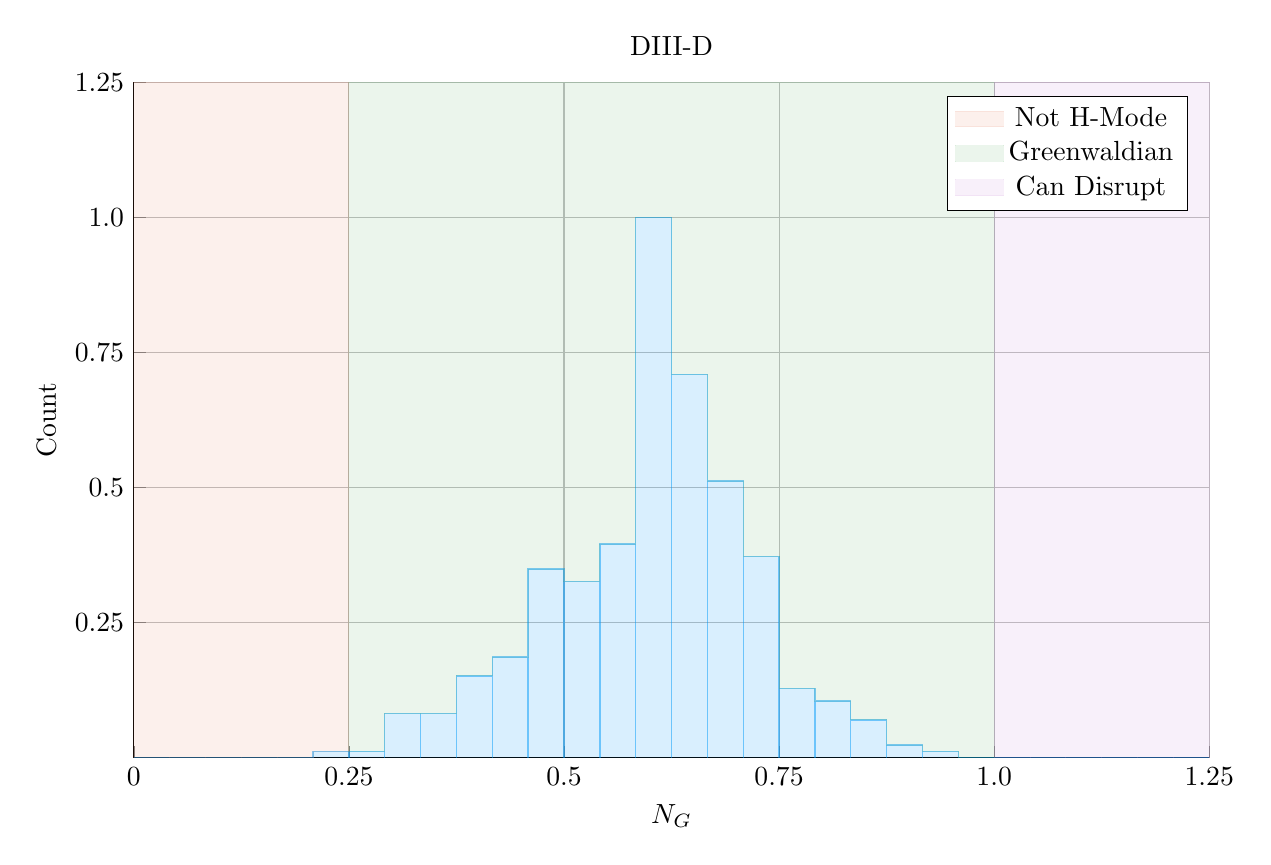
\begin{tikzpicture}[]
\begin{axis}[height = {101.6mm}, ylabel = {Count}, title = {DIII-D}, xmin = {0}, xmax = {1.25}, ymax = {1.25}, xlabel = {$N_G$}, {unbounded coords=jump, scaled x ticks = false, xticklabel style={rotate = 0}, xmajorgrids = true, xtick = {0.0,0.25,0.5,0.75,1.0,1.25}, xticklabels = {0,0.25,0.5,0.75,1.0,1.25}, xtick align = inside, axis lines* = left, scaled y ticks = false, yticklabel style={rotate = 0}, ymajorgrids = true, ytick = {0.0,0.25,0.5,0.75,1.0,1.25}, yticklabels = {,0.25,0.5,0.75,1.0,1.25}, ytick align = inside, axis lines* = left,     xshift = 0.0mm,
    yshift = 0.0mm,
    axis background/.style={fill={rgb,1:red,1.00000000;green,1.00000000;blue,1.00000000}}
}, ymin = {0}, width = {152.4mm}]\addplot+ [color = {rgb,1:red,0.00000000;green,0.60560316;blue,0.97868012},
draw opacity=0.5,
line width=0.5,
solid,mark = none,
mark size = 2.0,
mark options = {
    color = {rgb,1:red,0.00000000;green,0.00000000;blue,0.00000000}, draw opacity = 0.5,
    fill = {rgb,1:red,0.00000000;green,0.60560316;blue,0.97868012}, fill opacity = 0.5,
    line width = 1,
    rotate = 0,
    solid
},fill = {rgb,1:red,0.00000000;green,0.60560316;blue,0.97868012}, fill opacity=0.15,forget plot]coordinates {
(0.0, 0.0)
(0.0, 0.0)
(0.041666666666666664, 0.0)
(0.041666666666666664, 0.0)
(NaN, NaN)
(0.041666666666666664, 0.0)
(0.041666666666666664, 0.0)
(0.08333333333333333, 0.0)
(0.08333333333333333, 0.0)
(NaN, NaN)
(0.08333333333333333, 0.0)
(0.08333333333333333, 0.0)
(0.125, 0.0)
(0.125, 0.0)
(NaN, NaN)
(0.125, 0.0)
(0.125, 0.0)
(0.16666666666666666, 0.0)
(0.16666666666666666, 0.0)
(NaN, NaN)
(0.16666666666666666, 0.0)
(0.16666666666666666, 0.0)
(0.20833333333333334, 0.0)
(0.20833333333333334, 0.0)
(NaN, NaN)
(0.20833333333333334, 0.0)
(0.20833333333333334, 0.011627906976744186)
(0.25, 0.011627906976744186)
(0.25, 0.0)
(NaN, NaN)
(0.25, 0.0)
(0.25, 0.011627906976744186)
(0.2916666666666667, 0.011627906976744186)
(0.2916666666666667, 0.0)
(NaN, NaN)
(0.2916666666666667, 0.0)
(0.2916666666666667, 0.08139534883720931)
(0.3333333333333333, 0.08139534883720931)
(0.3333333333333333, 0.0)
(NaN, NaN)
(0.3333333333333333, 0.0)
(0.3333333333333333, 0.08139534883720931)
(0.375, 0.08139534883720931)
(0.375, 0.0)
(NaN, NaN)
(0.375, 0.0)
(0.375, 0.1511627906976744)
(0.4166666666666667, 0.1511627906976744)
(0.4166666666666667, 0.0)
(NaN, NaN)
(0.4166666666666667, 0.0)
(0.4166666666666667, 0.18604651162790697)
(0.4583333333333333, 0.18604651162790697)
(0.4583333333333333, 0.0)
(NaN, NaN)
(0.4583333333333333, 0.0)
(0.4583333333333333, 0.3488372093023256)
(0.5, 0.3488372093023256)
(0.5, 0.0)
(NaN, NaN)
(0.5, 0.0)
(0.5, 0.32558139534883723)
(0.5416666666666666, 0.32558139534883723)
(0.5416666666666666, 0.0)
(NaN, NaN)
(0.5416666666666666, 0.0)
(0.5416666666666666, 0.3953488372093023)
(0.5833333333333334, 0.3953488372093023)
(0.5833333333333334, 0.0)
(NaN, NaN)
(0.5833333333333334, 0.0)
(0.5833333333333334, 1.0)
(0.625, 1.0)
(0.625, 0.0)
(NaN, NaN)
(0.625, 0.0)
(0.625, 0.7093023255813954)
(0.6666666666666666, 0.7093023255813954)
(0.6666666666666666, 0.0)
(NaN, NaN)
(0.6666666666666666, 0.0)
(0.6666666666666666, 0.5116279069767442)
(0.7083333333333334, 0.5116279069767442)
(0.7083333333333334, 0.0)
(NaN, NaN)
(0.7083333333333334, 0.0)
(0.7083333333333334, 0.37209302325581395)
(0.75, 0.37209302325581395)
(0.75, 0.0)
(NaN, NaN)
(0.75, 0.0)
(0.75, 0.12790697674418605)
(0.7916666666666666, 0.12790697674418605)
(0.7916666666666666, 0.0)
(NaN, NaN)
(0.7916666666666666, 0.0)
(0.7916666666666666, 0.10465116279069768)
(0.8333333333333334, 0.10465116279069768)
(0.8333333333333334, 0.0)
(NaN, NaN)
(0.8333333333333334, 0.0)
(0.8333333333333334, 0.06976744186046512)
(0.875, 0.06976744186046512)
(0.875, 0.0)
(NaN, NaN)
(0.875, 0.0)
(0.875, 0.023255813953488372)
(0.9166666666666666, 0.023255813953488372)
(0.9166666666666666, 0.0)
(NaN, NaN)
(0.9166666666666666, 0.0)
(0.9166666666666666, 0.011627906976744186)
(0.9583333333333334, 0.011627906976744186)
(0.9583333333333334, 0.0)
(NaN, NaN)
(0.9583333333333334, 0.0)
(0.9583333333333334, 0.0)
(1.0, 0.0)
(1.0, 0.0)
(NaN, NaN)
(1.0, 0.0)
(1.0, 0.0)
(1.0416666666666667, 0.0)
(1.0416666666666667, 0.0)
(NaN, NaN)
(1.0416666666666667, 0.0)
(1.0416666666666667, 0.0)
(1.0833333333333333, 0.0)
(1.0833333333333333, 0.0)
(NaN, NaN)
(1.0833333333333333, 0.0)
(1.0833333333333333, 0.0)
(1.125, 0.0)
(1.125, 0.0)
(NaN, NaN)
(1.125, 0.0)
(1.125, 0.0)
(1.1666666666666667, 0.0)
(1.1666666666666667, 0.0)
(NaN, NaN)
(1.1666666666666667, 0.0)
(1.1666666666666667, 0.0)
(1.2083333333333333, 0.0)
(1.2083333333333333, 0.0)
(NaN, NaN)
(1.2083333333333333, 0.0)
(1.2083333333333333, 0.0)
(1.25, 0.0)
(1.25, 0.0)
(NaN, NaN)
};
\addplot+ [color = {rgb,1:red,0.88887350;green,0.43564919;blue,0.27812294},
draw opacity=0.1,
line width=0,
solid,mark = none,
mark size = 2.0,
mark options = {
    color = {rgb,1:red,0.00000000;green,0.00000000;blue,0.00000000}, draw opacity = 0.1,
    fill = {rgb,1:red,0.88887350;green,0.43564919;blue,0.27812294}, fill opacity = 0.1,
    line width = 1,
    rotate = 0,
    solid
},fill = {rgb,1:red,0.88887350;green,0.43564919;blue,0.27812294}, fill opacity=0.1,area legend]coordinates {
(0.0, 1.25)
(0.0, 0.0)
(0.041666666666666664, 0.0)
(0.041666666666666664, 0.0)
(0.08333333333333333, 0.0)
(0.08333333333333333, 0.0)
(0.125, 0.0)
(0.125, 0.0)
(0.16666666666666666, 0.0)
(0.16666666666666666, 0.0)
(0.20833333333333334, 0.0)
(0.20833333333333334, 0.011627906976744186)
(0.25, 0.011627906976744186)
(0.25, 1.25)
(0.0, 1.25)
};
\addlegendentry{Not H-Mode}
\addplot+ [color = {rgb,1:red,0.24222430;green,0.64327509;blue,0.30444865},
draw opacity=0.1,
line width=0,
solid,mark = none,
mark size = 2.0,
mark options = {
    color = {rgb,1:red,0.00000000;green,0.00000000;blue,0.00000000}, draw opacity = 0.1,
    fill = {rgb,1:red,0.24222430;green,0.64327509;blue,0.30444865}, fill opacity = 0.1,
    line width = 1,
    rotate = 0,
    solid
},fill = {rgb,1:red,0.24222430;green,0.64327509;blue,0.30444865}, fill opacity=0.1,area legend]coordinates {
(0.25, 1.25)
(0.25, 0.011627906976744186)
(0.2916666666666667, 0.011627906976744186)
(0.2916666666666667, 0.08139534883720931)
(0.3333333333333333, 0.08139534883720931)
(0.3333333333333333, 0.08139534883720931)
(0.375, 0.08139534883720931)
(0.375, 0.1511627906976744)
(0.4166666666666667, 0.1511627906976744)
(0.4166666666666667, 0.18604651162790697)
(0.4583333333333333, 0.18604651162790697)
(0.4583333333333333, 0.3488372093023256)
(0.5, 0.3488372093023256)
(0.5, 0.32558139534883723)
(0.5416666666666666, 0.32558139534883723)
(0.5416666666666666, 0.3953488372093023)
(0.5833333333333334, 0.3953488372093023)
(0.5833333333333334, 1.0)
(0.625, 1.0)
(0.625, 0.7093023255813954)
(0.6666666666666666, 0.7093023255813954)
(0.6666666666666666, 0.5116279069767442)
(0.7083333333333334, 0.5116279069767442)
(0.7083333333333334, 0.37209302325581395)
(0.75, 0.37209302325581395)
(0.75, 0.12790697674418605)
(0.7916666666666666, 0.12790697674418605)
(0.7916666666666666, 0.10465116279069768)
(0.8333333333333334, 0.10465116279069768)
(0.8333333333333334, 0.06976744186046512)
(0.875, 0.06976744186046512)
(0.875, 0.023255813953488372)
(0.9166666666666666, 0.023255813953488372)
(0.9166666666666666, 0.011627906976744186)
(0.9583333333333334, 0.011627906976744186)
(0.9583333333333334, 0.0)
(1.0, 0.0)
(1.0, 1.25)
(0.25, 1.25)
};
\addlegendentry{Greenwaldian}
\addplot+ [color = {rgb,1:red,0.76444018;green,0.44411178;blue,0.82429754},
draw opacity=0.1,
line width=0,
solid,mark = none,
mark size = 2.0,
mark options = {
    color = {rgb,1:red,0.00000000;green,0.00000000;blue,0.00000000}, draw opacity = 0.1,
    fill = {rgb,1:red,0.76444018;green,0.44411178;blue,0.82429754}, fill opacity = 0.1,
    line width = 1,
    rotate = 0,
    solid
},fill = {rgb,1:red,0.76444018;green,0.44411178;blue,0.82429754}, fill opacity=0.1,area legend]coordinates {
(1.0, 1.25)
(1.0, 0.0)
(1.0416666666666667, 0.0)
(1.0416666666666667, 0.0)
(1.0833333333333333, 0.0)
(1.0833333333333333, 0.0)
(1.125, 0.0)
(1.125, 0.0)
(1.1666666666666667, 0.0)
(1.1666666666666667, 0.0)
(1.2083333333333333, 0.0)
(1.2083333333333333, 0.0)
(1.25, 0.0)
(1.25, 1.25)
(1.0, 1.25)
};
\addlegendentry{Can Disrupt}
\end{axis}

\end{tikzpicture}

		\end{adjustbox}
        \caption{DIII-D}
    \end{subfigure}
    \hfill
    \begin{subfigure}[t]{0.45\textwidth}
        \centering
		\begin{adjustbox}{width=\textwidth}
			\Large
			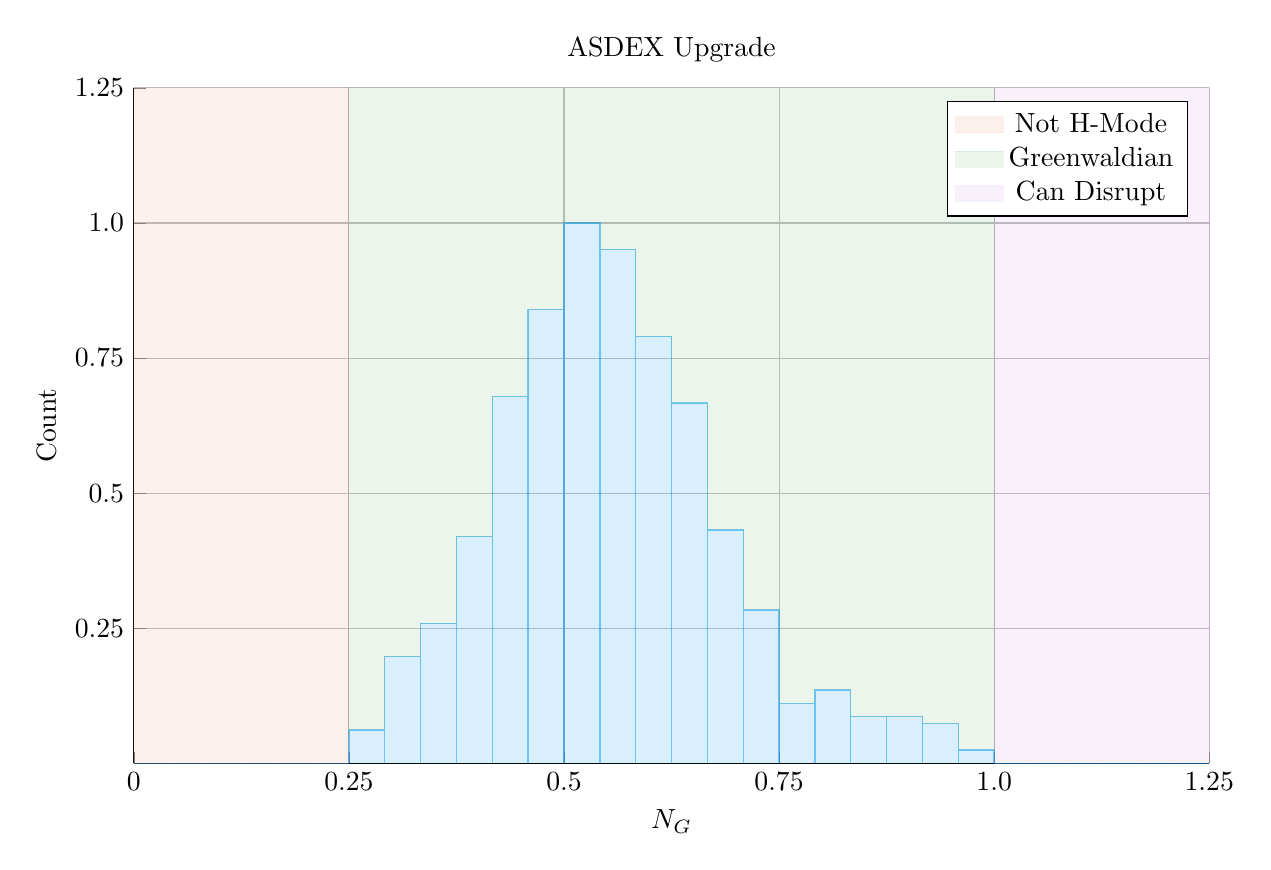
\begin{tikzpicture}[]
\begin{axis}[height = {101.6mm}, ylabel = {Count}, title = {ASDEX Upgrade}, xmin = {0}, xmax = {1.25}, ymax = {1.25}, xlabel = {$N_G$}, {unbounded coords=jump, scaled x ticks = false, xticklabel style={rotate = 0}, xmajorgrids = true, xtick = {0.0,0.25,0.5,0.75,1.0,1.25}, xticklabels = {0,0.25,0.5,0.75,1.0,1.25}, xtick align = inside, axis lines* = left, scaled y ticks = false, yticklabel style={rotate = 0}, ymajorgrids = true, ytick = {0.0,0.25,0.5,0.75,1.0,1.25}, yticklabels = {,0.25,0.5,0.75,1.0,1.25}, ytick align = inside, axis lines* = left,     xshift = 0.0mm,
    yshift = 0.0mm,
    axis background/.style={fill={rgb,1:red,1.00000000;green,1.00000000;blue,1.00000000}}
}, ymin = {0}, width = {152.4mm}]\addplot+ [color = {rgb,1:red,0.00000000;green,0.60560316;blue,0.97868012},
draw opacity=0.5,
line width=0.5,
solid,mark = none,
mark size = 2.0,
mark options = {
    color = {rgb,1:red,0.00000000;green,0.00000000;blue,0.00000000}, draw opacity = 0.5,
    fill = {rgb,1:red,0.00000000;green,0.60560316;blue,0.97868012}, fill opacity = 0.5,
    line width = 1,
    rotate = 0,
    solid
},fill = {rgb,1:red,0.00000000;green,0.60560316;blue,0.97868012}, fill opacity=0.15,forget plot]coordinates {
(0.0, 0.0)
(0.0, 0.0)
(0.041666666666666664, 0.0)
(0.041666666666666664, 0.0)
(NaN, NaN)
(0.041666666666666664, 0.0)
(0.041666666666666664, 0.0)
(0.08333333333333333, 0.0)
(0.08333333333333333, 0.0)
(NaN, NaN)
(0.08333333333333333, 0.0)
(0.08333333333333333, 0.0)
(0.125, 0.0)
(0.125, 0.0)
(NaN, NaN)
(0.125, 0.0)
(0.125, 0.0)
(0.16666666666666666, 0.0)
(0.16666666666666666, 0.0)
(NaN, NaN)
(0.16666666666666666, 0.0)
(0.16666666666666666, 0.0)
(0.20833333333333334, 0.0)
(0.20833333333333334, 0.0)
(NaN, NaN)
(0.20833333333333334, 0.0)
(0.20833333333333334, 0.0)
(0.25, 0.0)
(0.25, 0.0)
(NaN, NaN)
(0.25, 0.0)
(0.25, 0.06172839506172839)
(0.2916666666666667, 0.06172839506172839)
(0.2916666666666667, 0.0)
(NaN, NaN)
(0.2916666666666667, 0.0)
(0.2916666666666667, 0.19753086419753085)
(0.3333333333333333, 0.19753086419753085)
(0.3333333333333333, 0.0)
(NaN, NaN)
(0.3333333333333333, 0.0)
(0.3333333333333333, 0.25925925925925924)
(0.375, 0.25925925925925924)
(0.375, 0.0)
(NaN, NaN)
(0.375, 0.0)
(0.375, 0.41975308641975306)
(0.4166666666666667, 0.41975308641975306)
(0.4166666666666667, 0.0)
(NaN, NaN)
(0.4166666666666667, 0.0)
(0.4166666666666667, 0.6790123456790124)
(0.4583333333333333, 0.6790123456790124)
(0.4583333333333333, 0.0)
(NaN, NaN)
(0.4583333333333333, 0.0)
(0.4583333333333333, 0.8395061728395061)
(0.5, 0.8395061728395061)
(0.5, 0.0)
(NaN, NaN)
(0.5, 0.0)
(0.5, 1.0)
(0.5416666666666666, 1.0)
(0.5416666666666666, 0.0)
(NaN, NaN)
(0.5416666666666666, 0.0)
(0.5416666666666666, 0.9506172839506173)
(0.5833333333333334, 0.9506172839506173)
(0.5833333333333334, 0.0)
(NaN, NaN)
(0.5833333333333334, 0.0)
(0.5833333333333334, 0.7901234567901234)
(0.625, 0.7901234567901234)
(0.625, 0.0)
(NaN, NaN)
(0.625, 0.0)
(0.625, 0.6666666666666666)
(0.6666666666666666, 0.6666666666666666)
(0.6666666666666666, 0.0)
(NaN, NaN)
(0.6666666666666666, 0.0)
(0.6666666666666666, 0.43209876543209874)
(0.7083333333333334, 0.43209876543209874)
(0.7083333333333334, 0.0)
(NaN, NaN)
(0.7083333333333334, 0.0)
(0.7083333333333334, 0.2839506172839506)
(0.75, 0.2839506172839506)
(0.75, 0.0)
(NaN, NaN)
(0.75, 0.0)
(0.75, 0.1111111111111111)
(0.7916666666666666, 0.1111111111111111)
(0.7916666666666666, 0.0)
(NaN, NaN)
(0.7916666666666666, 0.0)
(0.7916666666666666, 0.13580246913580246)
(0.8333333333333334, 0.13580246913580246)
(0.8333333333333334, 0.0)
(NaN, NaN)
(0.8333333333333334, 0.0)
(0.8333333333333334, 0.08641975308641975)
(0.875, 0.08641975308641975)
(0.875, 0.0)
(NaN, NaN)
(0.875, 0.0)
(0.875, 0.08641975308641975)
(0.9166666666666666, 0.08641975308641975)
(0.9166666666666666, 0.0)
(NaN, NaN)
(0.9166666666666666, 0.0)
(0.9166666666666666, 0.07407407407407407)
(0.9583333333333334, 0.07407407407407407)
(0.9583333333333334, 0.0)
(NaN, NaN)
(0.9583333333333334, 0.0)
(0.9583333333333334, 0.024691358024691357)
(1.0, 0.024691358024691357)
(1.0, 0.0)
(NaN, NaN)
(1.0, 0.0)
(1.0, 0.0)
(1.0416666666666667, 0.0)
(1.0416666666666667, 0.0)
(NaN, NaN)
(1.0416666666666667, 0.0)
(1.0416666666666667, 0.0)
(1.0833333333333333, 0.0)
(1.0833333333333333, 0.0)
(NaN, NaN)
(1.0833333333333333, 0.0)
(1.0833333333333333, 0.0)
(1.125, 0.0)
(1.125, 0.0)
(NaN, NaN)
(1.125, 0.0)
(1.125, 0.0)
(1.1666666666666667, 0.0)
(1.1666666666666667, 0.0)
(NaN, NaN)
(1.1666666666666667, 0.0)
(1.1666666666666667, 0.0)
(1.2083333333333333, 0.0)
(1.2083333333333333, 0.0)
(NaN, NaN)
(1.2083333333333333, 0.0)
(1.2083333333333333, 0.0)
(1.25, 0.0)
(1.25, 0.0)
(NaN, NaN)
};
\addplot+ [color = {rgb,1:red,0.88887350;green,0.43564919;blue,0.27812294},
draw opacity=0.1,
line width=0,
solid,mark = none,
mark size = 2.0,
mark options = {
    color = {rgb,1:red,0.00000000;green,0.00000000;blue,0.00000000}, draw opacity = 0.1,
    fill = {rgb,1:red,0.88887350;green,0.43564919;blue,0.27812294}, fill opacity = 0.1,
    line width = 1,
    rotate = 0,
    solid
},fill = {rgb,1:red,0.88887350;green,0.43564919;blue,0.27812294}, fill opacity=0.1,area legend]coordinates {
(0.0, 1.25)
(0.0, 0.0)
(0.041666666666666664, 0.0)
(0.041666666666666664, 0.0)
(0.08333333333333333, 0.0)
(0.08333333333333333, 0.0)
(0.125, 0.0)
(0.125, 0.0)
(0.16666666666666666, 0.0)
(0.16666666666666666, 0.0)
(0.20833333333333334, 0.0)
(0.20833333333333334, 0.0)
(0.25, 0.0)
(0.25, 1.25)
(0.0, 1.25)
};
\addlegendentry{Not H-Mode}
\addplot+ [color = {rgb,1:red,0.24222430;green,0.64327509;blue,0.30444865},
draw opacity=0.1,
line width=0,
solid,mark = none,
mark size = 2.0,
mark options = {
    color = {rgb,1:red,0.00000000;green,0.00000000;blue,0.00000000}, draw opacity = 0.1,
    fill = {rgb,1:red,0.24222430;green,0.64327509;blue,0.30444865}, fill opacity = 0.1,
    line width = 1,
    rotate = 0,
    solid
},fill = {rgb,1:red,0.24222430;green,0.64327509;blue,0.30444865}, fill opacity=0.1,area legend]coordinates {
(0.25, 1.25)
(0.25, 0.06172839506172839)
(0.2916666666666667, 0.06172839506172839)
(0.2916666666666667, 0.19753086419753085)
(0.3333333333333333, 0.19753086419753085)
(0.3333333333333333, 0.25925925925925924)
(0.375, 0.25925925925925924)
(0.375, 0.41975308641975306)
(0.4166666666666667, 0.41975308641975306)
(0.4166666666666667, 0.6790123456790124)
(0.4583333333333333, 0.6790123456790124)
(0.4583333333333333, 0.8395061728395061)
(0.5, 0.8395061728395061)
(0.5, 1.0)
(0.5416666666666666, 1.0)
(0.5416666666666666, 0.9506172839506173)
(0.5833333333333334, 0.9506172839506173)
(0.5833333333333334, 0.7901234567901234)
(0.625, 0.7901234567901234)
(0.625, 0.6666666666666666)
(0.6666666666666666, 0.6666666666666666)
(0.6666666666666666, 0.43209876543209874)
(0.7083333333333334, 0.43209876543209874)
(0.7083333333333334, 0.2839506172839506)
(0.75, 0.2839506172839506)
(0.75, 0.1111111111111111)
(0.7916666666666666, 0.1111111111111111)
(0.7916666666666666, 0.13580246913580246)
(0.8333333333333334, 0.13580246913580246)
(0.8333333333333334, 0.08641975308641975)
(0.875, 0.08641975308641975)
(0.875, 0.08641975308641975)
(0.9166666666666666, 0.08641975308641975)
(0.9166666666666666, 0.07407407407407407)
(0.9583333333333334, 0.07407407407407407)
(0.9583333333333334, 0.024691358024691357)
(1.0, 0.024691358024691357)
(1.0, 1.25)
(0.25, 1.25)
};
\addlegendentry{Greenwaldian}
\addplot+ [color = {rgb,1:red,0.76444018;green,0.44411178;blue,0.82429754},
draw opacity=0.1,
line width=0,
solid,mark = none,
mark size = 2.0,
mark options = {
    color = {rgb,1:red,0.00000000;green,0.00000000;blue,0.00000000}, draw opacity = 0.1,
    fill = {rgb,1:red,0.76444018;green,0.44411178;blue,0.82429754}, fill opacity = 0.1,
    line width = 1,
    rotate = 0,
    solid
},fill = {rgb,1:red,0.76444018;green,0.44411178;blue,0.82429754}, fill opacity=0.1,area legend]coordinates {
(1.0, 1.25)
(1.0, 0.0)
(1.0416666666666667, 0.0)
(1.0416666666666667, 0.0)
(1.0833333333333333, 0.0)
(1.0833333333333333, 0.0)
(1.125, 0.0)
(1.125, 0.0)
(1.1666666666666667, 0.0)
(1.1666666666666667, 0.0)
(1.2083333333333333, 0.0)
(1.2083333333333333, 0.0)
(1.25, 0.0)
(1.25, 1.25)
(1.0, 1.25)
};
\addlegendentry{Can Disrupt}
\end{axis}

\end{tikzpicture}

		\end{adjustbox}
        \caption{ASDEX}
    \end{subfigure}
    \hfill \hfill ~\\ ~\\ ~\\
    \begin{subfigure}[t]{0.6\textwidth}
        \centering
		\begin{adjustbox}{width=\textwidth}
			\large
			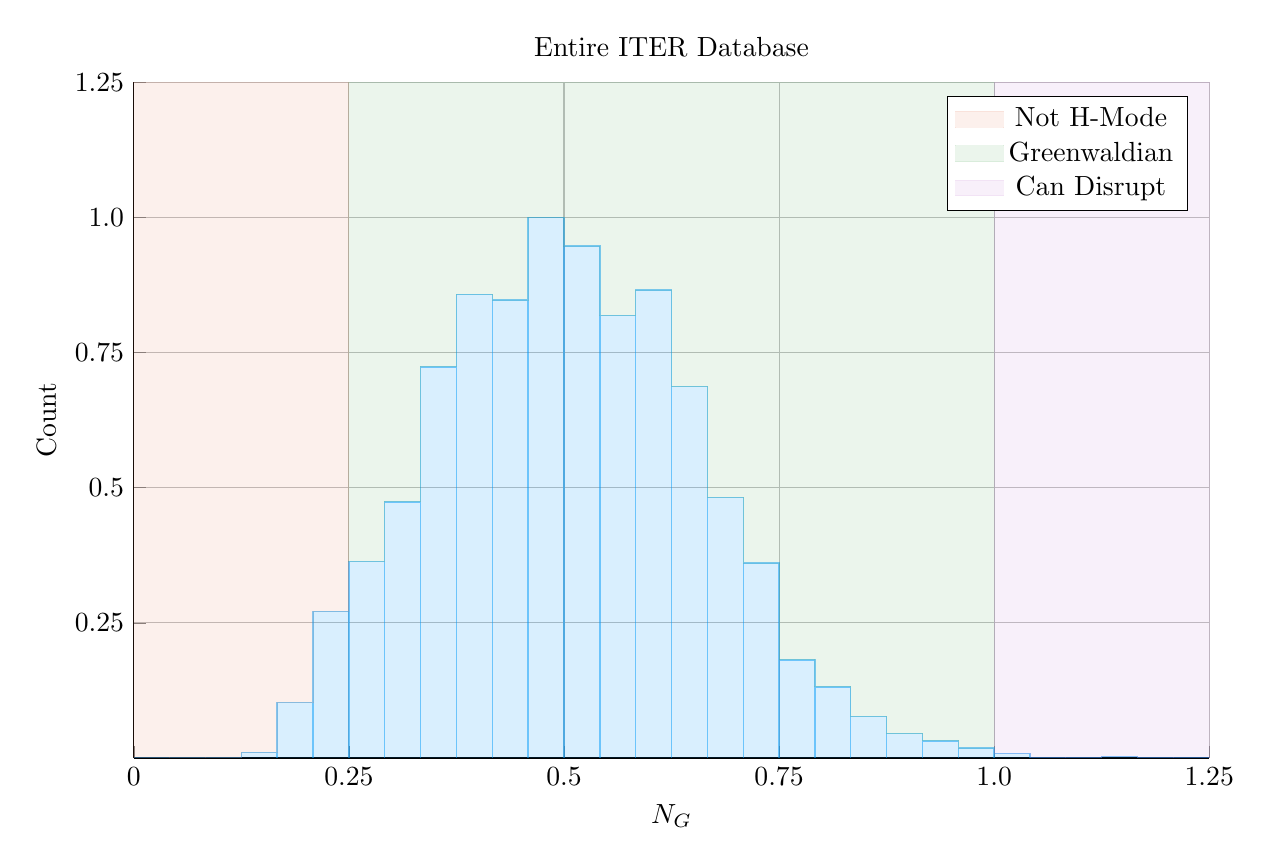
\begin{tikzpicture}[]
\begin{axis}[height = {101.6mm}, ylabel = {Count}, title = {Entire ITER Database}, xmin = {0}, xmax = {1.25}, ymax = {1.25}, xlabel = {$N_G$}, {unbounded coords=jump, scaled x ticks = false, xticklabel style={rotate = 0}, xmajorgrids = true, xtick = {0.0,0.25,0.5,0.75,1.0,1.25}, xticklabels = {0,0.25,0.5,0.75,1.0,1.25}, xtick align = inside, axis lines* = left, scaled y ticks = false, yticklabel style={rotate = 0}, ymajorgrids = true, ytick = {0.0,0.25,0.5,0.75,1.0,1.25}, yticklabels = {,0.25,0.5,0.75,1.0,1.25}, ytick align = inside, axis lines* = left,     xshift = 0.0mm,
    yshift = 0.0mm,
    axis background/.style={fill={rgb,1:red,1.00000000;green,1.00000000;blue,1.00000000}}
}, ymin = {0}, width = {152.4mm}]\addplot+ [color = {rgb,1:red,0.00000000;green,0.60560316;blue,0.97868012},
draw opacity=0.5,
line width=0.5,
solid,mark = none,
mark size = 2.0,
mark options = {
    color = {rgb,1:red,0.00000000;green,0.00000000;blue,0.00000000}, draw opacity = 0.5,
    fill = {rgb,1:red,0.00000000;green,0.60560316;blue,0.97868012}, fill opacity = 0.5,
    line width = 1,
    rotate = 0,
    solid
},fill = {rgb,1:red,0.00000000;green,0.60560316;blue,0.97868012}, fill opacity=0.15,forget plot]coordinates {
(0.0, 0.0)
(0.0, 0.0)
(0.041666666666666664, 0.0)
(0.041666666666666664, 0.0)
(NaN, NaN)
(0.041666666666666664, 0.0)
(0.041666666666666664, 0.0)
(0.08333333333333333, 0.0)
(0.08333333333333333, 0.0)
(NaN, NaN)
(0.08333333333333333, 0.0)
(0.08333333333333333, 0.0)
(0.125, 0.0)
(0.125, 0.0)
(NaN, NaN)
(0.125, 0.0)
(0.125, 0.010526315789473684)
(0.16666666666666666, 0.010526315789473684)
(0.16666666666666666, 0.0)
(NaN, NaN)
(0.16666666666666666, 0.0)
(0.16666666666666666, 0.10263157894736842)
(0.20833333333333334, 0.10263157894736842)
(0.20833333333333334, 0.0)
(NaN, NaN)
(0.20833333333333334, 0.0)
(0.20833333333333334, 0.2710526315789474)
(0.25, 0.2710526315789474)
(0.25, 0.0)
(NaN, NaN)
(0.25, 0.0)
(0.25, 0.3631578947368421)
(0.2916666666666667, 0.3631578947368421)
(0.2916666666666667, 0.0)
(NaN, NaN)
(0.2916666666666667, 0.0)
(0.2916666666666667, 0.47368421052631576)
(0.3333333333333333, 0.47368421052631576)
(0.3333333333333333, 0.0)
(NaN, NaN)
(0.3333333333333333, 0.0)
(0.3333333333333333, 0.7236842105263158)
(0.375, 0.7236842105263158)
(0.375, 0.0)
(NaN, NaN)
(0.375, 0.0)
(0.375, 0.8578947368421053)
(0.4166666666666667, 0.8578947368421053)
(0.4166666666666667, 0.0)
(NaN, NaN)
(0.4166666666666667, 0.0)
(0.4166666666666667, 0.8473684210526315)
(0.4583333333333333, 0.8473684210526315)
(0.4583333333333333, 0.0)
(NaN, NaN)
(0.4583333333333333, 0.0)
(0.4583333333333333, 1.0)
(0.5, 1.0)
(0.5, 0.0)
(NaN, NaN)
(0.5, 0.0)
(0.5, 0.9473684210526315)
(0.5416666666666666, 0.9473684210526315)
(0.5416666666666666, 0.0)
(NaN, NaN)
(0.5416666666666666, 0.0)
(0.5416666666666666, 0.8184210526315789)
(0.5833333333333334, 0.8184210526315789)
(0.5833333333333334, 0.0)
(NaN, NaN)
(0.5833333333333334, 0.0)
(0.5833333333333334, 0.8657894736842106)
(0.625, 0.8657894736842106)
(0.625, 0.0)
(NaN, NaN)
(0.625, 0.0)
(0.625, 0.6868421052631579)
(0.6666666666666666, 0.6868421052631579)
(0.6666666666666666, 0.0)
(NaN, NaN)
(0.6666666666666666, 0.0)
(0.6666666666666666, 0.48157894736842105)
(0.7083333333333334, 0.48157894736842105)
(0.7083333333333334, 0.0)
(NaN, NaN)
(0.7083333333333334, 0.0)
(0.7083333333333334, 0.3605263157894737)
(0.75, 0.3605263157894737)
(0.75, 0.0)
(NaN, NaN)
(0.75, 0.0)
(0.75, 0.18157894736842106)
(0.7916666666666666, 0.18157894736842106)
(0.7916666666666666, 0.0)
(NaN, NaN)
(0.7916666666666666, 0.0)
(0.7916666666666666, 0.13157894736842105)
(0.8333333333333334, 0.13157894736842105)
(0.8333333333333334, 0.0)
(NaN, NaN)
(0.8333333333333334, 0.0)
(0.8333333333333334, 0.07631578947368421)
(0.875, 0.07631578947368421)
(0.875, 0.0)
(NaN, NaN)
(0.875, 0.0)
(0.875, 0.04473684210526316)
(0.9166666666666666, 0.04473684210526316)
(0.9166666666666666, 0.0)
(NaN, NaN)
(0.9166666666666666, 0.0)
(0.9166666666666666, 0.031578947368421054)
(0.9583333333333334, 0.031578947368421054)
(0.9583333333333334, 0.0)
(NaN, NaN)
(0.9583333333333334, 0.0)
(0.9583333333333334, 0.018421052631578946)
(1.0, 0.018421052631578946)
(1.0, 0.0)
(NaN, NaN)
(1.0, 0.0)
(1.0, 0.007894736842105263)
(1.0416666666666667, 0.007894736842105263)
(1.0416666666666667, 0.0)
(NaN, NaN)
(1.0416666666666667, 0.0)
(1.0416666666666667, 0.0)
(1.0833333333333333, 0.0)
(1.0833333333333333, 0.0)
(NaN, NaN)
(1.0833333333333333, 0.0)
(1.0833333333333333, 0.0)
(1.125, 0.0)
(1.125, 0.0)
(NaN, NaN)
(1.125, 0.0)
(1.125, 0.002631578947368421)
(1.1666666666666667, 0.002631578947368421)
(1.1666666666666667, 0.0)
(NaN, NaN)
(1.1666666666666667, 0.0)
(1.1666666666666667, 0.0)
(1.2083333333333333, 0.0)
(1.2083333333333333, 0.0)
(NaN, NaN)
(1.2083333333333333, 0.0)
(1.2083333333333333, 0.0)
(1.25, 0.0)
(1.25, 0.0)
(NaN, NaN)
};
\addplot+ [color = {rgb,1:red,0.88887350;green,0.43564919;blue,0.27812294},
draw opacity=0.1,
line width=0,
solid,mark = none,
mark size = 2.0,
mark options = {
    color = {rgb,1:red,0.00000000;green,0.00000000;blue,0.00000000}, draw opacity = 0.1,
    fill = {rgb,1:red,0.88887350;green,0.43564919;blue,0.27812294}, fill opacity = 0.1,
    line width = 1,
    rotate = 0,
    solid
},fill = {rgb,1:red,0.88887350;green,0.43564919;blue,0.27812294}, fill opacity=0.1,area legend]coordinates {
(0.0, 1.25)
(0.0, 0.0)
(0.041666666666666664, 0.0)
(0.041666666666666664, 0.0)
(0.08333333333333333, 0.0)
(0.08333333333333333, 0.0)
(0.125, 0.0)
(0.125, 0.010526315789473684)
(0.16666666666666666, 0.010526315789473684)
(0.16666666666666666, 0.10263157894736842)
(0.20833333333333334, 0.10263157894736842)
(0.20833333333333334, 0.2710526315789474)
(0.25, 0.2710526315789474)
(0.25, 1.25)
(0.0, 1.25)
};
\addlegendentry{Not H-Mode}
\addplot+ [color = {rgb,1:red,0.24222430;green,0.64327509;blue,0.30444865},
draw opacity=0.1,
line width=0,
solid,mark = none,
mark size = 2.0,
mark options = {
    color = {rgb,1:red,0.00000000;green,0.00000000;blue,0.00000000}, draw opacity = 0.1,
    fill = {rgb,1:red,0.24222430;green,0.64327509;blue,0.30444865}, fill opacity = 0.1,
    line width = 1,
    rotate = 0,
    solid
},fill = {rgb,1:red,0.24222430;green,0.64327509;blue,0.30444865}, fill opacity=0.1,area legend]coordinates {
(0.25, 1.25)
(0.25, 0.3631578947368421)
(0.2916666666666667, 0.3631578947368421)
(0.2916666666666667, 0.47368421052631576)
(0.3333333333333333, 0.47368421052631576)
(0.3333333333333333, 0.7236842105263158)
(0.375, 0.7236842105263158)
(0.375, 0.8578947368421053)
(0.4166666666666667, 0.8578947368421053)
(0.4166666666666667, 0.8473684210526315)
(0.4583333333333333, 0.8473684210526315)
(0.4583333333333333, 1.0)
(0.5, 1.0)
(0.5, 0.9473684210526315)
(0.5416666666666666, 0.9473684210526315)
(0.5416666666666666, 0.8184210526315789)
(0.5833333333333334, 0.8184210526315789)
(0.5833333333333334, 0.8657894736842106)
(0.625, 0.8657894736842106)
(0.625, 0.6868421052631579)
(0.6666666666666666, 0.6868421052631579)
(0.6666666666666666, 0.48157894736842105)
(0.7083333333333334, 0.48157894736842105)
(0.7083333333333334, 0.3605263157894737)
(0.75, 0.3605263157894737)
(0.75, 0.18157894736842106)
(0.7916666666666666, 0.18157894736842106)
(0.7916666666666666, 0.13157894736842105)
(0.8333333333333334, 0.13157894736842105)
(0.8333333333333334, 0.07631578947368421)
(0.875, 0.07631578947368421)
(0.875, 0.04473684210526316)
(0.9166666666666666, 0.04473684210526316)
(0.9166666666666666, 0.031578947368421054)
(0.9583333333333334, 0.031578947368421054)
(0.9583333333333334, 0.018421052631578946)
(1.0, 0.018421052631578946)
(1.0, 1.25)
(0.25, 1.25)
};
\addlegendentry{Greenwaldian}
\addplot+ [color = {rgb,1:red,0.76444018;green,0.44411178;blue,0.82429754},
draw opacity=0.1,
line width=0,
solid,mark = none,
mark size = 2.0,
mark options = {
    color = {rgb,1:red,0.00000000;green,0.00000000;blue,0.00000000}, draw opacity = 0.1,
    fill = {rgb,1:red,0.76444018;green,0.44411178;blue,0.82429754}, fill opacity = 0.1,
    line width = 1,
    rotate = 0,
    solid
},fill = {rgb,1:red,0.76444018;green,0.44411178;blue,0.82429754}, fill opacity=0.1,area legend]coordinates {
(1.0, 1.25)
(1.0, 0.007894736842105263)
(1.0416666666666667, 0.007894736842105263)
(1.0416666666666667, 0.0)
(1.0833333333333333, 0.0)
(1.0833333333333333, 0.0)
(1.125, 0.0)
(1.125, 0.002631578947368421)
(1.1666666666666667, 0.002631578947368421)
(1.1666666666666667, 0.0)
(1.2083333333333333, 0.0)
(1.2083333333333333, 0.0)
(1.25, 0.0)
(1.25, 1.25)
(1.0, 1.25)
};
\addlegendentry{Can Disrupt}
\end{axis}

\end{tikzpicture}

		\end{adjustbox}
        \caption{All Tokamak Shots}
    \end{subfigure} ~\\ ~\\ ~\\
    \caption{Greenwald Density Limit} ~\\
    \small The Greenwald Density Limit is a robust metric of what densities an H-Mode plasma can attain. Although empirical in nature, it is an indicator for good transport regimes.
\end{figure*}

As no theoretical backing exists, the Greenwald density limit can simply be written (with citation) as: \cite{greenwald}

\begin{equation}
	\hat n = N_G \cdot \left( \frac{ I_P }{ \pi a^2} \right)
\end{equation}

Here, $\hat n$ has units of $10^{20} \ \frac{\textnormal{particles}}{\textnormal{m}^3}$, $N_G$ is the Greenwald density fraction, $I_P$ is again the plasma current (measured in mega-amps) and $\pi$ has its usual meaning (3.141592653...). The final variable is then the minor radius -- a -- which was previously defined through:

\begin{equation}
	\tag{\ref{eq:a}}
	a = \epsilon \cdot R_0
\end{equation}

The next step is transforming the \emph{line-averaged} density ($\hat n$) into the \emph{volume-averaged} version ($\overline n$) used in this model. Harnessing the simplicity of the density's parabolic profile allows this relation to be written in a closed form as:
 
 \begin{equation}
 	\hat n = \frac{\sqrt{\pi}}{2} \cdot \left( \frac{\Gamma \left( \nu_n + 2 \right)}{\Gamma \left( \nu_n + \frac{3}{2} \right)} \right) \cdot \overline n 
 \end{equation}
 
 Where $\Gamma( \, \cdots)$ represents the gamma function: the non-integer analogue of the factorial function.
 
 Combining these pieces allows the volume-averaged density to be written in standardized units (i.e. the ones we use) as:
 
 \begin{equation}
 	\label{eq:greenwald}
 	\tcbhighmath{
 	\overline n = K_n \cdot \left( \frac{I_P}{R_0^2} \right)
 	}
 \end{equation}
 \myequations{Greenwald Density -- $\overline n$}
 
 \begin{equation}
 	K_n = \frac{2 N_G}{\epsilon^2 \, \pi^{3/2} } \cdot \left( \frac{\Gamma \left( \nu_n + \frac{3}{2} \right)}{\Gamma \left( \nu_n + 2 \right)} \right)
\end{equation}
 
The format of the above equation pair will be used throughout the remainder of the paper. The top equation relates floating variables (i.e. $\overline n$, $I_P$, and $R_0$), while the fixed-value coefficient ($K_n$) lumps together fixed quantities, such as: $N_G$, $\epsilon$, 2, $\pi$, and $\nu_n$.

\subsection{Declaring the Bootstrap Current}

The first term to define in current balance, \cref{eq:ibal}, is the bootstrap current. This bootstrap current is a mechanism of tokamak plasmas that helps supply some of the current needed to keep a plasma stable. From a hand-waving perspective, it involves particles stuck in banana-shaped orbits on the outer edges of a tokamak behaving like racing-game style speed boosts that accelerate charged particles along their hooped-shaped race tracks.

To get an equation for bootstrap current, we must first introduce the surface integral -- made possible from our previous choice of geometric parameters:

\begin{equation}
	\label{eq:qs}
	Q_S = 2 \pi a^2 \kappa g \int_0^1 Q(\rho) \rho \, d\rho
\end{equation}
\myequations{Surface Integral -- $Q_S$}

Here, Q is an arbitrary function of the normalized radius ($\rho$) and g is a geometric factor (of order 1):

\begin{equation}
	g = \frac{1}{8} \cdot \left( 9 - 2 \delta - 0.3 \left( 1 - \delta^2 \right)  \right)
\end{equation}
 
This allows the bootstrap current ($I_{BS}$) to be written in terms of the temperature and density profiles:

\begin{equation}
	I_{BS} = 2 \pi a^2 \kappa g \int_0^1 J_{BS} \, \rho \, d\rho
\end{equation}

\begin{equation}
	J_{BS} = f\left( n , T , \frac{dn}{d\rho} , \frac{dT}{d\rho}  \right)
\end{equation}
 
For a more formal look into this $J_{BS}$ function, check the appendix section on pedestal temperatures. The point to make now is that it depends on the the profiles' derivatives, leading to one major discrepancy in the model. As shown later in the results, bootstrap fractions are often under-predicted by this model. This is due to parabolic profiles (i.e. for temperature) having much less steep declines near the edge (i.e. in their derivatives) than characteristic H-Mode profiles with pedestals. This implies that the area most positively impacted by a pedestal profile for temperature would be the bootstrap current derivation.

Getting back on track -- and without completeness -- the bootstrap current can now be written in proportionality form as:

\begin{equation}
	I_{BS} \propto \overline T \cdot \overline n \cdot \left( \frac{R_0^2}{I_P} \right)
\end{equation}

Recognizing that the last term is basically the inverse of the Greenwald density (see Eq. \ref{eq:greenwald}), allows the proportionality to be written in the following form. Note that this implies the bootstrap current is only a function of temperature!

\begin{equation}
	I_{BS} \propto K_n \cdot \overline T
\end{equation}

In standardized units, this proportionality can be written as a concrete relation of the form:

\begin{equation}
	\label{eq:ibs}
	\tcboxmath{
	I_{BS} = K_{BS} \cdot \overline T
	}
\end{equation}
\myequations{Bootstrap Current -- $I_{BS}$}

\begin{equation}
  K_{BS} = 4.879 \cdot  K_n \cdot \left( \, \frac{1+\kappa^2}{2} \, \right) \cdot \epsilon^{5/2} \cdot H_{BS}
\end{equation}

\begin{equation}
  H_{BS} = ( 1 + \nu_n ) ( 1 + \nu_T ) ( \nu_n + 0.054 \nu_T ) \int_0^1 \frac{ \rho^{\,5/2} \, ( \, 1 - \rho^{\,2} \, )^{\, \nu_n + \nu_T - 1} }{b_p} \, d\rho
\end{equation}

Quickly noting, this $H_{BS}$ term serves as the analogue of fixed-value coefficients (e.g. $K_{BS}$ and $K_n$) when they contain an integral. And $b_p$ represents the poloidal magnet strength given by Eq. \ref{eq:b_p}.

\subsection{Deriving the Fusion Power}

The next segue on our journey to solving for the steady current is deriving the fusion power ($P_F$), which appears in current drive. This requires a more first-principles approach than those used up until now. As such, a quick background is given to motivate the parameters it adds -- i.e. the dilution factor ($f_{D}$) and the Bosch-Hale fusion reactivity ($\sigma v$).

\begin{figure}
	\centering
	\begin{adjustbox}{width=0.75\textwidth}
		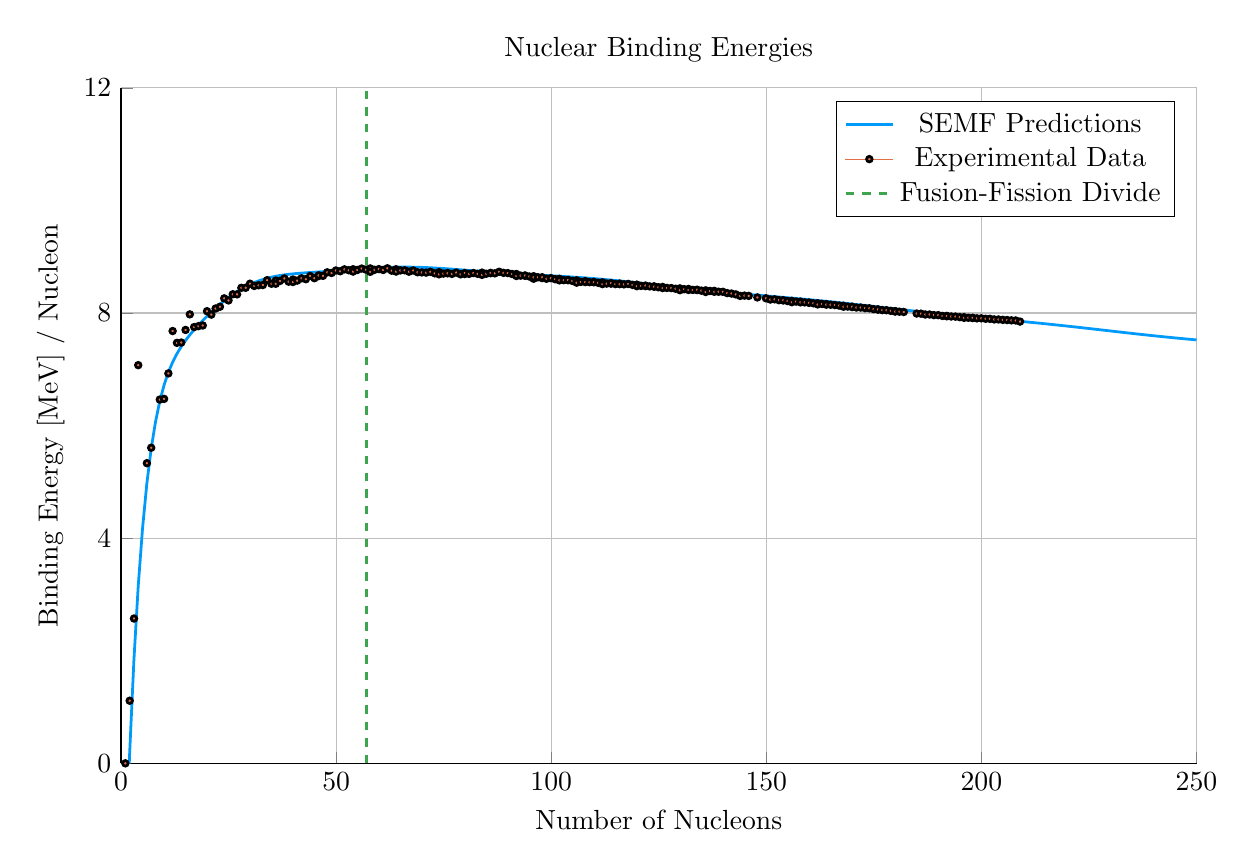
\begin{tikzpicture}[]
\begin{axis}[height = {101.6mm}, ylabel = {Binding Energy [MeV] / Nucleon}, title = {Nuclear Binding Energies}, xmin = {0}, xmax = {250}, ymax = {12}, xlabel = {Number of Nucleons}, {unbounded coords=jump, scaled x ticks = false, xticklabel style={rotate = 0}, xmajorgrids = true, xtick = {0.0,50.0,100.0,150.0,200.0,250.0}, xticklabels = {0,50,100,150,200,250}, xtick align = inside, axis lines* = left, scaled y ticks = false, yticklabel style={rotate = 0}, ymajorgrids = true, ytick = {0.0,4.0,8.0,12.0}, yticklabels = {0,4,8,12}, ytick align = inside, axis lines* = left,     xshift = 0.0mm,
    yshift = 0.0mm,
    axis background/.style={fill={rgb,1:red,1.00000000;green,1.00000000;blue,1.00000000}}
}, ymin = {0}, width = {152.4mm}]\addplot+ [color = {rgb,1:red,0.00000000;green,0.60560316;blue,0.97868012},
draw opacity=1.0,
line width=1,
solid,mark = none,
mark size = 2.0,
mark options = {
    color = {rgb,1:red,0.00000000;green,0.00000000;blue,0.00000000}, draw opacity = 1.0,
    fill = {rgb,1:red,0.00000000;green,0.60560316;blue,0.97868012}, fill opacity = 1.0,
    line width = 1,
    rotate = 0,
    solid
}]coordinates {
(0.0, -4.60355222317376)
(1.0, -1.9423714030316184)
(2.0, 0.17174117296689762)
(3.0, 1.84096399661781)
(4.0, 3.151140198415331)
(5.0, 4.173923283645508)
(6.0, 4.968707102167827)
(7.0, 5.58435286219236)
(8.0, 6.060726579422419)
(9.0, 6.430060629330575)
(10.0, 6.718153095546762)
(11.0, 6.9454184281365565)
(12.0, 7.127802582683796)
(13.0, 7.277575339898747)
(14.0, 7.404011936438574)
(15.0, 7.513975496904414)
(16.0, 7.6124110668622125)
(17.0, 7.702761326082542)
(18.0, 7.78731332582606)
(19.0, 7.867484857048368)
(20.0, 7.94405832862659)
(21.0, 8.017369324812918)
(22.0, 8.087456325980316)
(23.0, 8.154177421651507)
(24.0, 8.217299223743723)
(25.0, 8.276562603700583)
(26.0, 8.331729331502007)
(27.0, 8.382613188387339)
(28.0, 8.429098658726296)
(29.0, 8.471149879476823)
(30.0, 8.508812137244952)
(31.0, 8.542207851888847)
(32.0, 8.571528670372789)
(33.0, 8.59702501341144)
(34.0, 8.618994168442093)
(35.0, 8.637767803574754)
(36.0, 8.653699586296018)
(37.0, 8.66715342570664)
(38.0, 8.678492715810727)
(39.0, 8.688070837773061)
(40.0, 8.696223079017631)
(41.0, 8.703260044649955)
(42.0, 8.709462569971606)
(43.0, 8.715078090099894)
(44.0, 8.720318382160027)
(45.0, 8.725358565619327)
(46.0, 8.730337225625941)
(47.0, 8.735357511312394)
(48.0, 8.74048905473126)
(49.0, 8.745770555203375)
(50.0, 8.75121287745749)
(51.0, 8.756802519009028)
(52.0, 8.762505312039806)
(53.0, 8.76827023680805)
(54.0, 8.774033236747258)
(55.0, 8.779720939428142)
(56.0, 8.785254201806225)
(57.0, 8.790551412530785)
(58.0, 8.795531497975329)
(59.0, 8.800116592037245)
(60.0, 8.804234342184401)
(61.0, 8.80781983582066)
(62.0, 8.810817141406119)
(63.0, 8.813180468193043)
(64.0, 8.814874956307978)
(65.0, 8.815877115972366)
(66.0, 8.816174940266126)
(67.0, 8.815767720260371)
(68.0, 8.814665595039155)
(69.0, 8.81288887100591)
(70.0, 8.810467147004726)
(71.0, 8.807438281492448)
(72.0, 8.803847238531759)
(73.0, 8.799744847854736)
(74.0, 8.795186513048279)
(75.0, 8.790230899697235)
(76.0, 8.78493863297573)
(77.0, 8.77937103143497)
(78.0, 8.773588900376659)
(79.0, 8.767651405642294)
(80.0, 8.76161504469066)
(81.0, 8.755532729350353)
(82.0, 8.749452990095264)
(83.0, 8.743419310368836)
(84.0, 8.737469594886402)
(85.0, 8.731635772840807)
(86.0, 8.725943537136203)
(87.0, 8.72041221331207)
(88.0, 8.71505475533288)
(89.0, 8.709877858732526)
(90.0, 8.704882183589692)
(91.0, 8.700062675015097)
(92.0, 8.695408972428076)
(93.0, 8.690905892370129)
(94.0, 8.686533974543913)
(95.0, 8.682270076666686)
(96.0, 8.678088004492896)
(97.0, 8.67395916751817)
(98.0, 8.669853242580963)
(99.0, 8.665738837927783)
(100.0, 8.661584144823571)
(101.0, 8.657357563363785)
(102.0, 8.65302830389561)
(103.0, 8.648566937275728)
(104.0, 8.643945904303443)
(105.0, 8.639139972215713)
(106.0, 8.634126623930722)
(107.0, 8.628886396202454)
(108.0, 8.623403143699367)
(109.0, 8.617664241985338)
(110.0, 8.611660722384958)
(111.0, 8.605387333426602)
(112.0, 8.598842559648038)
(113.0, 8.592028549789976)
(114.0, 8.58495101272171)
(115.0, 8.57761904583371)
(116.0, 8.570044915671591)
(117.0, 8.562243798972087)
(118.0, 8.554233483777885)
(119.0, 8.546034047126547)
(120.0, 8.537667484888594)
(121.0, 8.52915735205801)
(122.0, 8.520528366411522)
(123.0, 8.511806023276883)
(124.0, 8.503016188183416)
(125.0, 8.494184739476726)
(126.0, 8.48533715574106)
(127.0, 8.476498181446992)
(128.0, 8.467691475241981)
(129.0, 8.458939312854039)
(130.0, 8.450262302915618)
(131.0, 8.441679114253642)
(132.0, 8.433206278428624)
(133.0, 8.424858004233645)
(134.0, 8.416646056664081)
(135.0, 8.408579640871974)
(136.0, 8.40066533194409)
(137.0, 8.392907065338754)
(138.0, 8.38530615381601)
(139.0, 8.377861360242079)
(140.0, 8.370568923080928)
(141.0, 8.363422766320568)
(142.0, 8.356414619878997)
(143.0, 8.349534089567673)
(144.0, 8.34276906318144)
(145.0, 8.336105786797518)
(146.0, 8.329529164601073)
(147.0, 8.323022920758717)
(148.0, 8.316570078748192)
(149.0, 8.310152950625312)
(150.0, 8.303753629008376)
(151.0, 8.297354097141259)
(152.0, 8.290936673163188)
(153.0, 8.284484104508877)
(154.0, 8.277979817957576)
(155.0, 8.271408214247263)
(156.0, 8.26475482066996)
(157.0, 8.258006702964753)
(158.0, 8.251151969185319)
(159.0, 8.244180856070077)
(160.0, 8.237085161410096)
(161.0, 8.229858338085972)
(162.0, 8.222496057535484)
(163.0, 8.214995696045428)
(164.0, 8.207356657383283)
(165.0, 8.199580440708676)
(166.0, 8.191669837642781)
(167.0, 8.183630071172871)
(168.0, 8.175467743710037)
(169.0, 8.167191164794605)
(170.0, 8.158809617848195)
(171.0, 8.150334504183075)
(172.0, 8.14177744744961)
(173.0, 8.133151658440163)
(174.0, 8.124470878350785)
(175.0, 8.115749356192289)
(176.0, 8.107001644999418)
(177.0, 8.098242201855552)
(178.0, 8.089486091809402)
(179.0, 8.080747293619883)
(180.0, 8.072039470032013)
(181.0, 8.063376210895715)
(182.0, 8.054769614767046)
(183.0, 8.0462311233693)
(184.0, 8.037770796191257)
(185.0, 8.029398175968147)
(186.0, 8.021119837562082)
(187.0, 8.012942869232848)
(188.0, 8.004870739363358)
(189.0, 7.996906945184318)
(190.0, 7.9890525617077115)
(191.0, 7.981307878966942)
(192.0, 7.973670320833624)
(193.0, 7.966137802437683)
(194.0, 7.9587038074885585)
(195.0, 7.951361389542597)
(196.0, 7.94410538135961)
(197.0, 7.936926816592529)
(198.0, 7.929813814345658)
(199.0, 7.9227553501678285)
(200.0, 7.9157413728397765)
(201.0, 7.908760790229455)
(202.0, 7.901797768231368)
(203.0, 7.894842094438137)
(204.0, 7.887880452358307)
(205.0, 7.880899530438714)
(206.0, 7.873885760576088)
(207.0, 7.866828874177291)
(208.0, 7.859716917643159)
(209.0, 7.8525395883864215)
(210.0, 7.845285908240645)
(211.0, 7.837951508078004)
(212.0, 7.830524697560121)
(213.0, 7.823000336600177)
(214.0, 7.815372950142774)
(215.0, 7.807640337638273)
(216.0, 7.799801848697318)
(217.0, 7.791862143087951)
(218.0, 7.783807545643804)
(219.0, 7.77565377827491)
(220.0, 7.767399807770702)
(221.0, 7.759051137290531)
(222.0, 7.750623260339327)
(223.0, 7.742107372543793)
(224.0, 7.73352368610323)
(225.0, 7.724889447747704)
(226.0, 7.7162018331861555)
(227.0, 7.707489994804505)
(228.0, 7.698747655296494)
(229.0, 7.689999393671084)
(230.0, 7.6812378105210035)
(231.0, 7.672517835584716)
(232.0, 7.663814423654281)
(233.0, 7.655151966005575)
(234.0, 7.646557126836435)
(235.0, 7.638013924639547)
(236.0, 7.629551857020474)
(237.0, 7.62119791263829)
(238.0, 7.612907202266693)
(239.0, 7.604745643355369)
(240.0, 7.596673359765863)
(241.0, 7.588747960772381)
(242.0, 7.580936729929124)
(243.0, 7.573223292898663)
(244.0, 7.565631417500911)
(245.0, 7.5581978936317435)
(246.0, 7.550821503884376)
(247.0, 7.543623555302642)
(248.0, 7.536478832551908)
(249.0, 7.529431955026017)
(250.0, 7.522541556397873)
};
\addlegendentry{SEMF Predictions}
\addplot+[draw=none, color = {rgb,1:red,0.88887350;green,0.43564919;blue,0.27812294},
draw opacity=1.0,
line width=0,
solid,mark = *,
mark size = 1.0,
mark options = {
    color = {rgb,1:red,0.00000000;green,0.00000000;blue,0.00000000}, draw opacity = 1.0,
    fill = {rgb,1:red,0.88887350;green,0.43564919;blue,0.27812294}, fill opacity = 1.0,
    line width = 1,
    rotate = 0,
    solid
}] coordinates {
(1.007825, 0.0)
(2.0141018, 1.1122865)
(3.0160293, 2.572686)
(4.0026032, 7.07391825)
(6.0151223, 5.332427333)
(7.016004, 5.606360857)
(9.0121821, 6.462767333)
(10.012937, 6.4750702)
(11.0093055, 6.927709364)
(12.0, 7.680145917)
(13.0033548, 7.469851)
(14.003074, 7.475616429)
(15.0001089, 7.699461867)
(15.9949146, 7.976208688)
(16.9991315, 7.750745)
(17.9991604, 7.7670585)
(18.9984032, 7.779019)
(19.9924402, 8.0322426)
(20.9938467, 7.971712381)
(21.9913855, 8.080450591)
(22.9897697, 8.111479391)
(23.9850419, 8.260703417)
(24.985837, 8.2235022)
(25.982593, 8.333870538)
(26.9815384, 8.331553704)
(27.9769265, 8.447745714)
(28.9764947, 8.448635759)
(29.9737702, 8.5206538)
(30.9737615, 8.481183452)
(31.9720707, 8.493145938)
(32.9714585, 8.497643667)
(33.9678668, 8.583505059)
(34.9688527, 8.520280229)
(35.9670809, 8.575386889)
(35.9675463, 8.5198805)
(36.9659026, 8.570282811)
(37.9627322, 8.614281105)
(38.9637069, 8.557018564)
(39.9623831, 8.595261375)
(39.9625912, 8.551298525)
(40.961826, 8.576058732)
(41.9586183, 8.616553905)
(42.9587668, 8.600656907)
(43.9554811, 8.658187182)
(44.9559102, 8.618876822)
(45.9526295, 8.656400587)
(45.9536928, 8.668884283)
(46.9517638, 8.661109447)
(47.9479471, 8.722890208)
(48.9478708, 8.711042755)
(49.9447921, 8.75560424)
(50.9439637, 8.741976863)
(51.9405119, 8.775867173)
(52.9406538, 8.760080585)
(53.9388849, 8.777838241)
(53.9396148, 8.736271611)
(54.9380496, 8.764914764)
(55.9349421, 8.790248321)
(56.9353987, 8.770174263)
(57.9332805, 8.792144241)
(57.9353479, 8.731962534)
(58.9332002, 8.767933983)
(59.9307906, 8.78069255)
(60.9310604, 8.764943607)
(61.9283488, 8.794496597)
(62.9296011, 8.752082952)
(63.9279696, 8.777416234)
(63.9291466, 8.735836984)
(64.9277937, 8.757037815)
(65.9260368, 8.759590848)
(66.9271309, 8.734107179)
(67.9248476, 8.755637676)
(68.9255809, 8.724482)
(69.9242504, 8.721679686)
(70.924705, 8.717574859)
(71.9220762, 8.731742861)
(72.9234594, 8.705046356)
(73.9211782, 8.725197459)
(73.9224766, 8.6877095)
(74.9215964, 8.70085368)
(75.9192141, 8.711474776)
(75.9214027, 8.705237934)
(76.9199146, 8.694687091)
(77.9173095, 8.717805526)
(78.9183376, 8.68759657)
(79.916378, 8.6929306)
(79.9165218, 8.710815425)
(80.9162911, 8.695915321)
(81.9134846, 8.71063828)
(82.914136, 8.695625024)
(83.9115066, 8.717350548)
(83.9134248, 8.677451726)
(84.9117893, 8.697447294)
(85.9092624, 8.708440733)
(85.9106103, 8.712034709)
(86.9088793, 8.705218437)
(87.9056143, 8.732575159)
(88.9058479, 8.713910393)
(89.9047037, 8.709920922)
(90.905645, 8.693268154)
(91.9050401, 8.692631598)
(91.9068105, 8.657698924)
(92.9063775, 8.66414257)
(93.9050876, 8.662296372)
(93.9063158, 8.666771426)
(94.9058415, 8.648682926)
(95.9046789, 8.65394974)
(95.9075977, 8.609329219)
(95.9082757, 8.635348635)
(96.906021, 8.635054443)
(97.9052871, 8.620312122)
(97.9054078, 8.635130592)
(98.9059393, 8.608630253)
(99.9042197, 8.61927551)
(100.9055822, 8.601283307)
(101.9043495, 8.607345284)
(101.9056077, 8.580514941)
(102.9055042, 8.584102893)
(103.9040349, 8.584809519)
(103.9054301, 8.587358327)
(104.905084, 8.570611867)
(105.9034831, 8.579970453)
(105.906458, 8.539066528)
(106.905093, 8.553889477)
(107.9038945, 8.567003037)
(107.9041834, 8.550022833)
(108.9047555, 8.547919321)
(109.9030056, 8.551293391)
(109.9051524, 8.547338309)
(110.9041816, 8.537100027)
(111.9027572, 8.544787813)
(111.9048208, 8.513654438)
(112.9040612, 8.522924912)
(113.9027818, 8.522555167)
(113.9033581, 8.531571772)
(114.903346, 8.514061435)
(115.9017441, 8.523107595)
(115.9047554, 8.512415397)
(116.9029538, 8.509615906)
(117.9016063, 8.516538458)
(118.9033089, 8.499470176)
(119.9021966, 8.504536442)
(119.9040199, 8.47734375)
(120.903818, 8.48200724)
(121.9030471, 8.478115393)
(121.9034401, 8.487940057)
(122.9042157, 8.472318821)
(123.9028195, 8.473263645)
(123.9052746, 8.467438726)
(124.9044247, 8.458085936)
(125.9033055, 8.463290746)
(125.9042689, 8.443750778)
(126.9044684, 8.445514346)
(127.9035304, 8.443305016)
(128.9047795, 8.431402163)
(129.9035079, 8.437744138)
(129.9063105, 8.4056265)
(130.9050819, 8.423754511)
(131.9041545, 8.427628947)
(131.9050562, 8.409412727)
(132.9054469, 8.41001582)
(133.9045033, 8.40820859)
(133.9053945, 8.413690821)
(134.9056827, 8.39757577)
(135.9045701, 8.402797926)
(135.9071436, 8.373666206)
(136.9058214, 8.391869759)
(137.9052413, 8.39346358)
(137.9059856, 8.377100848)
(138.9063482, 8.37809918)
(139.905434, 8.376402064)
(140.9076477, 8.354065376)
(141.9077186, 8.346099423)
(142.9098096, 8.330557867)
(143.9119947, 8.303756715)
(144.9125688, 8.309256297)
(145.9131121, 8.30416076)
(147.9168885, 8.277245601)
(149.9172715, 8.26169108)
(150.919846, 8.239366947)
(151.9197282, 8.244130184)
(152.9212262, 8.228767745)
(153.9208623, 8.224866201)
(153.9222053, 8.226903344)
(154.9226188, 8.213319839)
(155.9221196, 8.215390718)
(155.9242783, 8.192470455)
(156.9239567, 8.203572854)
(157.9241005, 8.20188807)
(157.9244046, 8.190191728)
(158.9253431, 8.188866572)
(159.9251937, 8.184111788)
(159.9270506, 8.183081056)
(160.9269296, 8.173367894)
(161.9267947, 8.173513907)
(161.9287749, 8.152468833)
(162.9287275, 8.16184127)
(163.9291712, 8.158769561)
(163.929197, 8.149082091)
(164.9303192, 8.147017042)
(165.93029, 8.142011898)
(166.9320454, 8.131797198)
(167.9323678, 8.129650298)
(167.9338945, 8.111871631)
(168.9342111, 8.114515675)
(169.9347587, 8.106659294)
(169.9354603, 8.112018182)
(170.9363223, 8.097934655)
(171.9363777, 8.097480244)
(172.9382068, 8.087480665)
(173.9388581, 8.083900891)
(174.9407679, 8.069192943)
(175.9414018, 8.061404835)
(175.9425684, 8.064120898)
(176.94322, 8.051892299)
(177.9436977, 8.049501567)
(178.9458151, 8.038604905)
(179.9465488, 8.0349901)
(179.9467057, 8.025484889)
(180.9479963, 8.023418619)
(181.9482055, 8.01831256)
(184.9529557, 7.991024865)
(185.9543622, 7.988619242)
(186.9557479, 7.973791439)
(187.955836, 7.973874356)
(188.9581449, 7.963010111)
(189.9584452, 7.962108089)
(190.9605912, 7.94811756)
(191.9610352, 7.942530948)
(191.961479, 7.948527021)
(192.9629237, 7.938136917)
(193.9626636, 7.936039562)
(194.9647744, 7.926650138)
(195.9649349, 7.926625776)
(195.9658148, 7.914460474)
(196.9665516, 7.915744218)
(197.9667518, 7.911637121)
(197.967876, 7.914250535)
(198.9682625, 7.905367905)
(199.9683087, 7.905982665)
(200.9702853, 7.897644955)
(201.9706256, 7.896935792)
(202.9723291, 7.886124034)
(203.9734756, 7.885631485)
(204.9744123, 7.87846501)
(205.974449, 7.87543732)
(206.9758806, 7.869941454)
(207.9766359, 7.867527303)
(208.9803832, 7.848057507)
};
\addlegendentry{Experimental Data}
\addplot+ [color = {rgb,1:red,0.24222430;green,0.64327509;blue,0.30444865},
draw opacity=1.0,
line width=1,
dashed,mark = none,
mark size = 2.0,
mark options = {
    color = {rgb,1:red,0.00000000;green,0.00000000;blue,0.00000000}, draw opacity = 1.0,
    fill = {rgb,1:red,0.24222430;green,0.64327509;blue,0.30444865}, fill opacity = 1.0,
    line width = 1,
    rotate = 0,
    solid
}]coordinates {
(57, 0)
(57, 12)
};
\addlegendentry{Fusion-Fission Divide}
\end{axis}

\end{tikzpicture}

	\end{adjustbox}
%	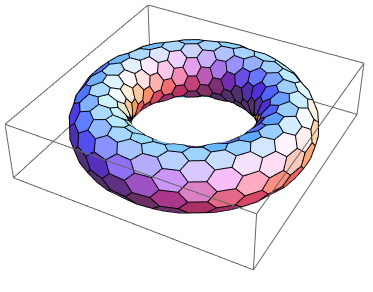
\includegraphics[width=0.75\textwidth]{images/test_image}
	\caption{Comparing Nuclear Fusion and Fission} ~\\
	\small The binding energy per nucleon is what differentiates nuclear fusion from fission. Nuclei heavier than Iron fission (e.g. Uranium), while light ones -- such as Hydrogen -- fuse. 
	\label{fig:binding_energy}
\end{figure}

The natural place to start when talking about fusion is the binding-energy per nucleon plot (see \cref{fig:binding_energy}). As can be seen, the function reaches a maximum value around the element Iron (A=56). What this means at a basic level is: elements lighter than iron can \emph{fuse} into a heavier one (i.e. hydrogens into helium), whereas heavier elements can \emph{fission} into lighter ones (e.g. uranium into krypton and barium). This is what differentiates fission (uranium-fueled) reactors from fusion (hydrogen-fueled) ones. For fusion reactors, the most common reaction in a first-generation tokamak will be:

\begin{equation}
	{}^2H+ {}^3H \rightarrow {}^4 He + {}^1 n + E_F
\end{equation}
\myequations{Fusion Energy -- $E_F$}

\begin{equation}
	E_F = 17.6 \ \textnormal{MeV}
\end{equation}

What this reaction describes is two isotopes of hydrogen -- i.e. deuterium and tritium -- fusing into a heavier element, helium, while simultaneously ejecting a neutron. The entire energy of the fusion reaction ($E_F$) is then divvied up 80-20 between the neutron and helium, respectively. Quantitatively, the helium (hereafter referred to as an alpha particle) receives 3.5 MeV.

\begin{figure}
	\centering
	\begin{adjustbox}{width=0.75\textwidth}
		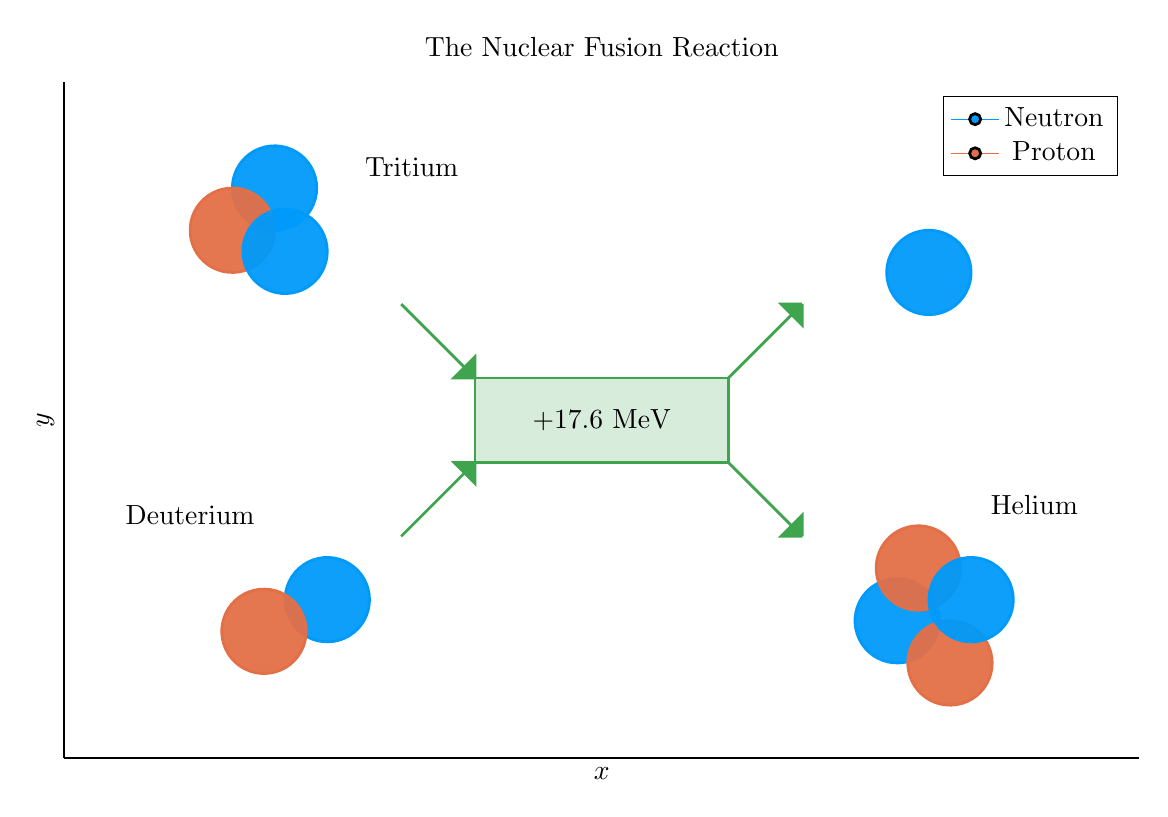
\begin{tikzpicture}[]
\begin{axis}[height = {101.6mm}, axis equal = {true}, ylabel = {$y$}, title = {The Nuclear Fusion Reaction}, xmin = {-12}, xmax = {12}, ymax = {8}, xlabel = {$x$}, {unbounded coords=jump, scaled x ticks = false, xticklabel style={rotate = 0}, xmajorticks=false, xmajorgrids = false, axis lines* = left, scaled y ticks = false, yticklabel style={rotate = 0}, ymajorticks=false, ymajorgrids = false, axis lines* = left,     xshift = 0.0mm,
    yshift = 0.0mm,
    axis background/.style={fill={rgb,1:red,1.00000000;green,1.00000000;blue,1.00000000}}
}, ymin = {-8}, width = {152.4mm}]\addplot+ [color = {rgb,1:red,0.00000000;green,0.60560316;blue,0.97868012},
draw opacity=1.0,
line width=1,
solid,mark = none,
mark size = 2.0,
mark options = {
    color = {rgb,1:red,0.00000000;green,0.00000000;blue,0.00000000}, draw opacity = 1.0,
    fill = {rgb,1:red,0.00000000;green,0.60560316;blue,0.97868012}, fill opacity = 1.0,
    line width = 1,
    rotate = 0,
    solid
},fill = {rgb,1:red,0.00000000;green,0.60560316;blue,0.97868012}, fill opacity=0.95,forget plot]coordinates {
(-6.75, 5.5)
(-6.7582099861767535, 5.627877161684506)
(-6.7827051369609705, 5.7536545839095075)
(-6.823083242653978, 5.875267004879374)
(-6.878681295876611, 5.990717552003938)
(-6.948586378132044, 6.0981105304912155)
(-7.031650649902272, 6.195682550603486)
(-7.126510198141267, 6.2818314824680295)
(-7.231607431689475, 6.355142763005346)
(-7.345216656877606, 6.414412623015813)
(-7.465472413368968, 6.45866785303666)
(-7.590400104966621, 6.48718178341445)
(-7.717948422428345, 6.499486216200688)
(-7.846023025907682, 6.495379112949198)
(-7.972520933956314, 6.4749279121818235)
(-8.095365054421308, 6.438468422049761)
(-8.212538290240834, 6.386599306373)
(-8.32211666012217, 6.320172254596956)
(-8.422300890261317, 6.2402779970753155)
(-8.511445958369134, 6.148228395307789)
(-8.58808810489184, 6.045534901210549)
(-8.650968867902419, 5.933883739117558)
(-8.699055747010668, 5.815108218023621)
(-8.731559156991064, 5.6911586287013725)
(-8.747945392750337, 5.564070219980713)
(-8.747945392750337, 5.435929780019287)
(-8.731559156991064, 5.3088413712986275)
(-8.699055747010668, 5.184891781976379)
(-8.650968867902419, 5.066116260882442)
(-8.58808810489184, 4.954465098789451)
(-8.511445958369135, 4.851771604692212)
(-8.422300890261317, 4.7597220029246845)
(-8.32211666012217, 4.679827745403045)
(-8.212538290240836, 4.613400693627)
(-8.095365054421308, 4.56153157795024)
(-7.972520933956314, 4.5250720878181765)
(-7.846023025907682, 4.504620887050802)
(-7.7179484224283454, 4.500513783799312)
(-7.590400104966621, 4.51281821658555)
(-7.465472413368968, 4.541332146963339)
(-7.345216656877606, 4.585587376984187)
(-7.231607431689476, 4.644857236994653)
(-7.126510198141267, 4.71816851753197)
(-7.031650649902272, 4.804317449396514)
(-6.948586378132044, 4.901889469508784)
(-6.878681295876611, 5.009282447996062)
(-6.823083242653978, 5.124732995120626)
(-6.7827051369609705, 5.2463454160904925)
(-6.7582099861767535, 5.3721228383154935)
(-6.75, 5.5)
};
\addplot+ [color = {rgb,1:red,0.88887350;green,0.43564919;blue,0.27812294},
draw opacity=1.0,
line width=1,
solid,mark = none,
mark size = 2.0,
mark options = {
    color = {rgb,1:red,0.00000000;green,0.00000000;blue,0.00000000}, draw opacity = 1.0,
    fill = {rgb,1:red,0.88887350;green,0.43564919;blue,0.27812294}, fill opacity = 1.0,
    line width = 1,
    rotate = 0,
    solid
},fill = {rgb,1:red,0.88887350;green,0.43564919;blue,0.27812294}, fill opacity=0.95,forget plot]coordinates {
(-7.75, 4.5)
(-7.7582099861767535, 4.627877161684506)
(-7.7827051369609705, 4.7536545839095075)
(-7.823083242653978, 4.875267004879374)
(-7.878681295876611, 4.990717552003938)
(-7.948586378132044, 5.0981105304912155)
(-8.031650649902272, 5.195682550603486)
(-8.126510198141267, 5.2818314824680295)
(-8.231607431689476, 5.355142763005346)
(-8.345216656877605, 5.414412623015813)
(-8.465472413368968, 5.45866785303666)
(-8.590400104966621, 5.48718178341445)
(-8.717948422428345, 5.499486216200688)
(-8.846023025907682, 5.495379112949198)
(-8.972520933956314, 5.4749279121818235)
(-9.095365054421308, 5.438468422049761)
(-9.212538290240834, 5.386599306373)
(-9.32211666012217, 5.320172254596956)
(-9.422300890261317, 5.2402779970753155)
(-9.511445958369134, 5.148228395307789)
(-9.58808810489184, 5.045534901210549)
(-9.650968867902419, 4.933883739117558)
(-9.699055747010668, 4.815108218023621)
(-9.731559156991064, 4.6911586287013725)
(-9.747945392750337, 4.564070219980713)
(-9.747945392750337, 4.435929780019287)
(-9.731559156991064, 4.3088413712986275)
(-9.699055747010668, 4.184891781976379)
(-9.650968867902419, 4.066116260882442)
(-9.58808810489184, 3.9544650987894516)
(-9.511445958369135, 3.8517716046922117)
(-9.422300890261317, 3.7597220029246845)
(-9.32211666012217, 3.6798277454030446)
(-9.212538290240836, 3.613400693627)
(-9.095365054421308, 3.5615315779502397)
(-8.972520933956314, 3.5250720878181765)
(-8.846023025907682, 3.5046208870508018)
(-8.717948422428345, 3.5005137837993123)
(-8.590400104966621, 3.5128182165855497)
(-8.465472413368968, 3.541332146963339)
(-8.345216656877607, 3.5855873769841873)
(-8.231607431689476, 3.6448572369946537)
(-8.126510198141267, 3.71816851753197)
(-8.031650649902272, 3.804317449396514)
(-7.948586378132044, 3.9018894695087836)
(-7.878681295876611, 4.009282447996062)
(-7.823083242653978, 4.124732995120626)
(-7.7827051369609705, 4.2463454160904925)
(-7.7582099861767535, 4.3721228383154935)
(-7.75, 4.5)
};
\addplot+ [color = {rgb,1:red,0.00000000;green,0.60560316;blue,0.97868012},
draw opacity=1.0,
line width=1,
solid,mark = none,
mark size = 2.0,
mark options = {
    color = {rgb,1:red,0.00000000;green,0.00000000;blue,0.00000000}, draw opacity = 1.0,
    fill = {rgb,1:red,0.00000000;green,0.60560316;blue,0.97868012}, fill opacity = 1.0,
    line width = 1,
    rotate = 0,
    solid
},fill = {rgb,1:red,0.00000000;green,0.60560316;blue,0.97868012}, fill opacity=0.95,forget plot]coordinates {
(-6.5, 4.0)
(-6.5082099861767535, 4.127877161684506)
(-6.5327051369609705, 4.2536545839095075)
(-6.573083242653978, 4.375267004879374)
(-6.628681295876611, 4.490717552003938)
(-6.698586378132044, 4.5981105304912155)
(-6.781650649902272, 4.695682550603486)
(-6.876510198141267, 4.7818314824680295)
(-6.981607431689475, 4.855142763005346)
(-7.095216656877606, 4.914412623015813)
(-7.215472413368968, 4.95866785303666)
(-7.340400104966621, 4.98718178341445)
(-7.467948422428345, 4.999486216200688)
(-7.596023025907682, 4.995379112949198)
(-7.722520933956314, 4.9749279121818235)
(-7.845365054421308, 4.938468422049761)
(-7.962538290240835, 4.886599306373)
(-8.07211666012217, 4.820172254596956)
(-8.172300890261317, 4.7402779970753155)
(-8.261445958369134, 4.648228395307789)
(-8.33808810489184, 4.545534901210549)
(-8.400968867902419, 4.433883739117558)
(-8.449055747010668, 4.315108218023621)
(-8.481559156991064, 4.1911586287013725)
(-8.497945392750337, 4.064070219980713)
(-8.497945392750337, 3.935929780019287)
(-8.481559156991064, 3.8088413712986275)
(-8.449055747010668, 3.6848917819763796)
(-8.400968867902419, 3.566116260882442)
(-8.33808810489184, 3.4544650987894516)
(-8.261445958369135, 3.3517716046922117)
(-8.172300890261317, 3.2597220029246845)
(-8.07211666012217, 3.1798277454030446)
(-7.962538290240835, 3.113400693627)
(-7.8453650544213085, 3.0615315779502397)
(-7.722520933956314, 3.0250720878181765)
(-7.596023025907682, 3.0046208870508018)
(-7.4679484224283454, 3.0005137837993123)
(-7.340400104966621, 3.0128182165855497)
(-7.215472413368968, 3.041332146963339)
(-7.095216656877606, 3.0855873769841873)
(-6.981607431689476, 3.1448572369946537)
(-6.876510198141267, 3.21816851753197)
(-6.781650649902272, 3.304317449396514)
(-6.698586378132044, 3.4018894695087836)
(-6.628681295876611, 3.5092824479960623)
(-6.573083242653978, 3.6247329951206253)
(-6.5327051369609705, 3.7463454160904925)
(-6.5082099861767535, 3.8721228383154935)
(-6.5, 3.9999999999999996)
};
\addplot+ [color = {rgb,1:red,0.00000000;green,0.60560316;blue,0.97868012},
draw opacity=1.0,
line width=1,
solid,mark = none,
mark size = 2.0,
mark options = {
    color = {rgb,1:red,0.00000000;green,0.00000000;blue,0.00000000}, draw opacity = 1.0,
    fill = {rgb,1:red,0.00000000;green,0.60560316;blue,0.97868012}, fill opacity = 1.0,
    line width = 1,
    rotate = 0,
    solid
},fill = {rgb,1:red,0.00000000;green,0.60560316;blue,0.97868012}, fill opacity=0.95,forget plot]coordinates {
(-5.5, -4.25)
(-5.5082099861767535, -4.122122838315494)
(-5.5327051369609705, -3.9963454160904925)
(-5.573083242653978, -3.8747329951206257)
(-5.628681295876611, -3.7592824479960623)
(-5.698586378132044, -3.651889469508784)
(-5.781650649902272, -3.5543174493965135)
(-5.876510198141267, -3.46816851753197)
(-5.981607431689475, -3.394857236994654)
(-6.095216656877606, -3.3355873769841873)
(-6.215472413368968, -3.2913321469633394)
(-6.340400104966621, -3.2628182165855497)
(-6.467948422428345, -3.2505137837993123)
(-6.596023025907682, -3.2546208870508018)
(-6.722520933956314, -3.2750720878181765)
(-6.845365054421308, -3.3115315779502397)
(-6.962538290240835, -3.363400693627)
(-7.07211666012217, -3.429827745403044)
(-7.172300890261317, -3.5097220029246845)
(-7.261445958369134, -3.6017716046922117)
(-7.338088104891841, -3.704465098789451)
(-7.400968867902419, -3.816116260882442)
(-7.449055747010669, -3.934891781976379)
(-7.481559156991065, -4.0588413712986275)
(-7.497945392750337, -4.185929780019287)
(-7.497945392750337, -4.314070219980713)
(-7.481559156991065, -4.4411586287013725)
(-7.449055747010669, -4.565108218023621)
(-7.400968867902419, -4.683883739117558)
(-7.338088104891841, -4.795534901210549)
(-7.261445958369134, -4.898228395307788)
(-7.172300890261317, -4.9902779970753155)
(-7.07211666012217, -5.070172254596955)
(-6.962538290240835, -5.136599306373)
(-6.8453650544213085, -5.18846842204976)
(-6.722520933956314, -5.2249279121818235)
(-6.596023025907682, -5.245379112949198)
(-6.4679484224283454, -5.249486216200688)
(-6.340400104966621, -5.23718178341445)
(-6.215472413368968, -5.208667853036661)
(-6.095216656877606, -5.164412623015813)
(-5.981607431689476, -5.105142763005347)
(-5.876510198141267, -5.03183148246803)
(-5.781650649902272, -4.945682550603486)
(-5.698586378132044, -4.848110530491216)
(-5.628681295876611, -4.740717552003938)
(-5.573083242653978, -4.625267004879374)
(-5.5327051369609705, -4.5036545839095075)
(-5.5082099861767535, -4.3778771616845065)
(-5.5, -4.25)
};
\addplot+ [color = {rgb,1:red,0.88887350;green,0.43564919;blue,0.27812294},
draw opacity=1.0,
line width=1,
solid,mark = none,
mark size = 2.0,
mark options = {
    color = {rgb,1:red,0.00000000;green,0.00000000;blue,0.00000000}, draw opacity = 1.0,
    fill = {rgb,1:red,0.88887350;green,0.43564919;blue,0.27812294}, fill opacity = 1.0,
    line width = 1,
    rotate = 0,
    solid
},fill = {rgb,1:red,0.88887350;green,0.43564919;blue,0.27812294}, fill opacity=0.95,forget plot]coordinates {
(-7.0, -5.0)
(-7.0082099861767535, -4.872122838315494)
(-7.0327051369609705, -4.7463454160904925)
(-7.073083242653978, -4.624732995120626)
(-7.128681295876611, -4.509282447996062)
(-7.198586378132044, -4.4018894695087845)
(-7.281650649902272, -4.304317449396514)
(-7.376510198141267, -4.2181685175319705)
(-7.481607431689475, -4.144857236994654)
(-7.595216656877606, -4.085587376984187)
(-7.715472413368968, -4.04133214696334)
(-7.840400104966621, -4.01281821658555)
(-7.967948422428345, -4.000513783799312)
(-8.096023025907682, -4.004620887050802)
(-8.222520933956314, -4.0250720878181765)
(-8.345365054421308, -4.061531577950239)
(-8.462538290240834, -4.113400693627)
(-8.57211666012217, -4.179827745403044)
(-8.672300890261317, -4.2597220029246845)
(-8.761445958369134, -4.351771604692211)
(-8.83808810489184, -4.454465098789451)
(-8.900968867902419, -4.566116260882442)
(-8.949055747010668, -4.684891781976379)
(-8.981559156991064, -4.8088413712986275)
(-8.997945392750337, -4.935929780019287)
(-8.997945392750337, -5.064070219980713)
(-8.981559156991064, -5.1911586287013725)
(-8.949055747010668, -5.315108218023621)
(-8.900968867902419, -5.433883739117558)
(-8.83808810489184, -5.545534901210549)
(-8.761445958369135, -5.648228395307788)
(-8.672300890261317, -5.7402779970753155)
(-8.57211666012217, -5.820172254596955)
(-8.462538290240836, -5.886599306373)
(-8.345365054421308, -5.93846842204976)
(-8.222520933956314, -5.9749279121818235)
(-8.096023025907682, -5.995379112949198)
(-7.9679484224283454, -5.999486216200688)
(-7.840400104966621, -5.98718178341445)
(-7.715472413368968, -5.958667853036661)
(-7.595216656877606, -5.914412623015813)
(-7.481607431689476, -5.855142763005347)
(-7.376510198141267, -5.78183148246803)
(-7.281650649902272, -5.695682550603486)
(-7.198586378132044, -5.598110530491216)
(-7.128681295876611, -5.490717552003938)
(-7.073083242653978, -5.375267004879374)
(-7.0327051369609705, -5.2536545839095075)
(-7.0082099861767535, -5.1278771616845065)
(-7.0, -5.0)
};
\addplot+ [color = {rgb,1:red,0.24222430;green,0.64327509;blue,0.30444865},
draw opacity=1.0,
line width=1,
solid,mark = none,
mark size = 2.0,
mark options = {
    color = {rgb,1:red,0.00000000;green,0.00000000;blue,0.00000000}, draw opacity = 1.0,
    fill = {rgb,1:red,0.24222430;green,0.64327509;blue,0.30444865}, fill opacity = 1.0,
    line width = 1,
    rotate = 0,
    solid
},forget plot]coordinates {
(-4.75, 2.75)
(-3.0, 1.0)
};
\addplot+ [color = {rgb,1:red,0.24222430;green,0.64327509;blue,0.30444865},
draw opacity=1.0,
line width=1,
solid,mark = none,
mark size = 2.0,
mark options = {
    color = {rgb,1:red,0.00000000;green,0.00000000;blue,0.00000000}, draw opacity = 1.0,
    fill = {rgb,1:red,0.24222430;green,0.64327509;blue,0.30444865}, fill opacity = 1.0,
    line width = 1,
    rotate = 0,
    solid
},forget plot]coordinates {
(-4.75, -2.75)
(-3.0, -1.0)
};
\addplot+ [color = {rgb,1:red,0.24222430;green,0.64327509;blue,0.30444865},
draw opacity=1.0,
line width=1,
solid,mark = none,
mark size = 2.0,
mark options = {
    color = {rgb,1:red,0.00000000;green,0.00000000;blue,0.00000000}, draw opacity = 1.0,
    fill = {rgb,1:red,0.24222430;green,0.64327509;blue,0.30444865}, fill opacity = 1.0,
    line width = 1,
    rotate = 0,
    solid
},fill = {rgb,1:red,0.24222430;green,0.64327509;blue,0.30444865}, fill opacity=1.0,forget plot]coordinates {
(-3.0, 1.0)
(-3.5, 1.0)
(-3.0, 1.5)
(-3.0, 1.0)
};
\addplot+ [color = {rgb,1:red,0.24222430;green,0.64327509;blue,0.30444865},
draw opacity=1.0,
line width=1,
solid,mark = none,
mark size = 2.0,
mark options = {
    color = {rgb,1:red,0.00000000;green,0.00000000;blue,0.00000000}, draw opacity = 1.0,
    fill = {rgb,1:red,0.24222430;green,0.64327509;blue,0.30444865}, fill opacity = 1.0,
    line width = 1,
    rotate = 0,
    solid
},fill = {rgb,1:red,0.24222430;green,0.64327509;blue,0.30444865}, fill opacity=1.0,forget plot]coordinates {
(-3.0, -1.0)
(-3.5, -1.0)
(-3.0, -1.5)
(-3.0, -1.0)
};
\addplot+ [color = {rgb,1:red,0.24222430;green,0.64327509;blue,0.30444865},
draw opacity=1.0,
line width=1,
solid,mark = none,
mark size = 2.0,
mark options = {
    color = {rgb,1:red,0.00000000;green,0.00000000;blue,0.00000000}, draw opacity = 1.0,
    fill = {rgb,1:red,0.24222430;green,0.64327509;blue,0.30444865}, fill opacity = 1.0,
    line width = 1,
    rotate = 0,
    solid
},forget plot]coordinates {
(3.0, 1.0)
(4.75, 2.75)
};
\addplot+ [color = {rgb,1:red,0.24222430;green,0.64327509;blue,0.30444865},
draw opacity=1.0,
line width=1,
solid,mark = none,
mark size = 2.0,
mark options = {
    color = {rgb,1:red,0.00000000;green,0.00000000;blue,0.00000000}, draw opacity = 1.0,
    fill = {rgb,1:red,0.24222430;green,0.64327509;blue,0.30444865}, fill opacity = 1.0,
    line width = 1,
    rotate = 0,
    solid
},forget plot]coordinates {
(3.0, -1.0)
(4.75, -2.75)
};
\addplot+ [color = {rgb,1:red,0.24222430;green,0.64327509;blue,0.30444865},
draw opacity=1.0,
line width=1,
solid,mark = none,
mark size = 2.0,
mark options = {
    color = {rgb,1:red,0.00000000;green,0.00000000;blue,0.00000000}, draw opacity = 1.0,
    fill = {rgb,1:red,0.24222430;green,0.64327509;blue,0.30444865}, fill opacity = 1.0,
    line width = 1,
    rotate = 0,
    solid
},fill = {rgb,1:red,0.24222430;green,0.64327509;blue,0.30444865}, fill opacity=1.0,forget plot]coordinates {
(4.75, 2.75)
(4.25, 2.75)
(4.75, 2.25)
(4.75, 2.75)
};
\addplot+ [color = {rgb,1:red,0.24222430;green,0.64327509;blue,0.30444865},
draw opacity=1.0,
line width=1,
solid,mark = none,
mark size = 2.0,
mark options = {
    color = {rgb,1:red,0.00000000;green,0.00000000;blue,0.00000000}, draw opacity = 1.0,
    fill = {rgb,1:red,0.24222430;green,0.64327509;blue,0.30444865}, fill opacity = 1.0,
    line width = 1,
    rotate = 0,
    solid
},fill = {rgb,1:red,0.24222430;green,0.64327509;blue,0.30444865}, fill opacity=1.0,forget plot]coordinates {
(4.75, -2.75)
(4.25, -2.75)
(4.75, -2.25)
(4.75, -2.75)
};
\addplot+ [color = {rgb,1:red,0.24222430;green,0.64327509;blue,0.30444865},
draw opacity=1.0,
line width=1,
solid,mark = none,
mark size = 2.0,
mark options = {
    color = {rgb,1:red,0.00000000;green,0.00000000;blue,0.00000000}, draw opacity = 1.0,
    fill = {rgb,1:red,0.24222430;green,0.64327509;blue,0.30444865}, fill opacity = 1.0,
    line width = 1,
    rotate = 0,
    solid
},fill = {rgb,1:red,0.24222430;green,0.64327509;blue,0.30444865}, fill opacity=0.2,forget plot]coordinates {
(-3, 1)
(3, 1)
(3, -1)
(-3, -1)
(-3, 1)
};
\addplot+ [color = {rgb,1:red,0.00000000;green,0.60560316;blue,0.97868012},
draw opacity=1.0,
line width=1,
solid,mark = none,
mark size = 2.0,
mark options = {
    color = {rgb,1:red,0.00000000;green,0.00000000;blue,0.00000000}, draw opacity = 1.0,
    fill = {rgb,1:red,0.00000000;green,0.60560316;blue,0.97868012}, fill opacity = 1.0,
    line width = 1,
    rotate = 0,
    solid
},fill = {rgb,1:red,0.00000000;green,0.60560316;blue,0.97868012}, fill opacity=0.95,forget plot]coordinates {
(8.75, 3.5)
(8.741790013823246, 3.627877161684506)
(8.71729486303903, 3.7536545839095075)
(8.67691675734602, 3.8752670048793743)
(8.62131870412339, 3.9907175520039377)
(8.551413621867956, 4.0981105304912155)
(8.468349350097728, 4.195682550603486)
(8.373489801858733, 4.2818314824680295)
(8.268392568310524, 4.355142763005346)
(8.154783343122395, 4.414412623015813)
(8.034527586631032, 4.45866785303666)
(7.909599895033379, 4.48718178341445)
(7.782051577571655, 4.499486216200688)
(7.653976974092318, 4.495379112949198)
(7.527479066043686, 4.4749279121818235)
(7.404634945578692, 4.438468422049761)
(7.287461709759165, 4.386599306373)
(7.17788333987783, 4.320172254596956)
(7.077699109738683, 4.2402779970753155)
(6.988554041630866, 4.148228395307789)
(6.911911895108159, 4.045534901210549)
(6.849031132097581, 3.933883739117558)
(6.800944252989331, 3.815108218023621)
(6.768440843008935, 3.6911586287013725)
(6.752054607249663, 3.5640702199807133)
(6.752054607249663, 3.435929780019287)
(6.768440843008935, 3.3088413712986275)
(6.800944252989331, 3.1848917819763796)
(6.849031132097581, 3.066116260882442)
(6.911911895108159, 2.9544650987894516)
(6.988554041630866, 2.8517716046922117)
(7.077699109738683, 2.7597220029246845)
(7.17788333987783, 2.6798277454030446)
(7.287461709759165, 2.613400693627)
(7.4046349455786915, 2.5615315779502397)
(7.527479066043686, 2.5250720878181765)
(7.653976974092318, 2.5046208870508018)
(7.7820515775716546, 2.5005137837993123)
(7.909599895033379, 2.5128182165855497)
(8.034527586631032, 2.541332146963339)
(8.154783343122393, 2.5855873769841873)
(8.268392568310524, 2.6448572369946537)
(8.373489801858733, 2.71816851753197)
(8.468349350097728, 2.804317449396514)
(8.551413621867956, 2.9018894695087836)
(8.62131870412339, 3.0092824479960623)
(8.67691675734602, 3.1247329951206253)
(8.71729486303903, 3.2463454160904925)
(8.741790013823246, 3.3721228383154935)
(8.75, 3.4999999999999996)
};
\addplot+ [color = {rgb,1:red,0.00000000;green,0.60560316;blue,0.97868012},
draw opacity=1.0,
line width=1,
solid,mark = none,
mark size = 2.0,
mark options = {
    color = {rgb,1:red,0.00000000;green,0.00000000;blue,0.00000000}, draw opacity = 1.0,
    fill = {rgb,1:red,0.00000000;green,0.60560316;blue,0.97868012}, fill opacity = 1.0,
    line width = 1,
    rotate = 0,
    solid
},fill = {rgb,1:red,0.00000000;green,0.60560316;blue,0.97868012}, fill opacity=0.95,forget plot]coordinates {
(8.0, -4.75)
(7.9917900138232465, -4.622122838315494)
(7.9672948630390295, -4.4963454160904925)
(7.926916757346022, -4.374732995120626)
(7.871318704123389, -4.259282447996062)
(7.801413621867956, -4.1518894695087845)
(7.718349350097728, -4.054317449396514)
(7.623489801858733, -3.96816851753197)
(7.518392568310525, -3.894857236994654)
(7.404783343122394, -3.8355873769841873)
(7.284527586631032, -3.7913321469633394)
(7.159599895033379, -3.7628182165855497)
(7.032051577571655, -3.7505137837993123)
(6.903976974092318, -3.7546208870508018)
(6.777479066043686, -3.7750720878181765)
(6.654634945578692, -3.8115315779502397)
(6.537461709759165, -3.863400693627)
(6.42788333987783, -3.929827745403044)
(6.327699109738683, -4.0097220029246845)
(6.238554041630866, -4.101771604692211)
(6.161911895108159, -4.204465098789451)
(6.099031132097581, -4.316116260882442)
(6.050944252989331, -4.434891781976379)
(6.018440843008935, -4.5588413712986275)
(6.002054607249663, -4.685929780019287)
(6.002054607249663, -4.814070219980713)
(6.018440843008935, -4.9411586287013725)
(6.050944252989331, -5.065108218023621)
(6.099031132097581, -5.183883739117558)
(6.161911895108159, -5.295534901210549)
(6.238554041630866, -5.398228395307788)
(6.327699109738683, -5.4902779970753155)
(6.42788333987783, -5.570172254596955)
(6.537461709759165, -5.636599306373)
(6.6546349455786915, -5.68846842204976)
(6.777479066043686, -5.7249279121818235)
(6.903976974092318, -5.745379112949198)
(7.0320515775716546, -5.749486216200688)
(7.159599895033379, -5.73718178341445)
(7.284527586631032, -5.708667853036661)
(7.404783343122394, -5.664412623015813)
(7.518392568310524, -5.605142763005347)
(7.623489801858733, -5.53183148246803)
(7.718349350097728, -5.445682550603486)
(7.801413621867956, -5.348110530491216)
(7.871318704123389, -5.240717552003938)
(7.926916757346022, -5.125267004879374)
(7.9672948630390295, -5.0036545839095075)
(7.9917900138232465, -4.8778771616845065)
(8.0, -4.75)
};
\addplot+ [color = {rgb,1:red,0.88887350;green,0.43564919;blue,0.27812294},
draw opacity=1.0,
line width=1,
solid,mark = none,
mark size = 2.0,
mark options = {
    color = {rgb,1:red,0.00000000;green,0.00000000;blue,0.00000000}, draw opacity = 1.0,
    fill = {rgb,1:red,0.88887350;green,0.43564919;blue,0.27812294}, fill opacity = 1.0,
    line width = 1,
    rotate = 0,
    solid
},fill = {rgb,1:red,0.88887350;green,0.43564919;blue,0.27812294}, fill opacity=0.95,forget plot]coordinates {
(9.25, -5.75)
(9.241790013823246, -5.622122838315494)
(9.21729486303903, -5.4963454160904925)
(9.17691675734602, -5.374732995120626)
(9.12131870412339, -5.259282447996062)
(9.051413621867956, -5.1518894695087845)
(8.968349350097728, -5.054317449396514)
(8.873489801858733, -4.9681685175319705)
(8.768392568310524, -4.894857236994654)
(8.654783343122395, -4.835587376984187)
(8.534527586631032, -4.79133214696334)
(8.409599895033379, -4.76281821658555)
(8.282051577571655, -4.750513783799312)
(8.153976974092318, -4.754620887050802)
(8.027479066043686, -4.7750720878181765)
(7.904634945578692, -4.811531577950239)
(7.787461709759165, -4.863400693627)
(7.67788333987783, -4.929827745403044)
(7.577699109738683, -5.0097220029246845)
(7.488554041630866, -5.101771604692211)
(7.411911895108159, -5.204465098789451)
(7.349031132097581, -5.316116260882442)
(7.300944252989331, -5.434891781976379)
(7.268440843008935, -5.5588413712986275)
(7.252054607249663, -5.685929780019287)
(7.252054607249663, -5.814070219980713)
(7.268440843008935, -5.9411586287013725)
(7.300944252989331, -6.065108218023621)
(7.349031132097581, -6.183883739117558)
(7.411911895108159, -6.295534901210549)
(7.488554041630866, -6.398228395307788)
(7.577699109738683, -6.4902779970753155)
(7.67788333987783, -6.570172254596955)
(7.787461709759165, -6.636599306373)
(7.9046349455786915, -6.68846842204976)
(8.027479066043686, -6.7249279121818235)
(8.153976974092318, -6.745379112949198)
(8.282051577571655, -6.749486216200688)
(8.409599895033379, -6.73718178341445)
(8.534527586631032, -6.708667853036661)
(8.654783343122393, -6.664412623015813)
(8.768392568310524, -6.605142763005347)
(8.873489801858733, -6.53183148246803)
(8.968349350097728, -6.445682550603486)
(9.051413621867956, -6.348110530491216)
(9.12131870412339, -6.240717552003938)
(9.17691675734602, -6.125267004879374)
(9.21729486303903, -6.0036545839095075)
(9.241790013823246, -5.8778771616845065)
(9.25, -5.75)
};
\addplot+ [color = {rgb,1:red,0.88887350;green,0.43564919;blue,0.27812294},
draw opacity=1.0,
line width=1,
solid,mark = none,
mark size = 2.0,
mark options = {
    color = {rgb,1:red,0.00000000;green,0.00000000;blue,0.00000000}, draw opacity = 1.0,
    fill = {rgb,1:red,0.88887350;green,0.43564919;blue,0.27812294}, fill opacity = 1.0,
    line width = 1,
    rotate = 0,
    solid
},fill = {rgb,1:red,0.88887350;green,0.43564919;blue,0.27812294}, fill opacity=0.95,forget plot]coordinates {
(8.5, -3.5)
(8.491790013823246, -3.372122838315494)
(8.46729486303903, -3.2463454160904925)
(8.42691675734602, -3.1247329951206257)
(8.37131870412339, -3.0092824479960623)
(8.301413621867956, -2.901889469508784)
(8.218349350097728, -2.8043174493965135)
(8.123489801858733, -2.71816851753197)
(8.018392568310524, -2.644857236994654)
(7.904783343122394, -2.5855873769841873)
(7.784527586631032, -2.5413321469633394)
(7.659599895033379, -2.5128182165855497)
(7.532051577571655, -2.5005137837993123)
(7.403976974092318, -2.5046208870508018)
(7.277479066043686, -2.5250720878181765)
(7.154634945578692, -2.5615315779502397)
(7.037461709759165, -2.613400693627)
(6.92788333987783, -2.679827745403044)
(6.827699109738683, -2.7597220029246845)
(6.738554041630866, -2.8517716046922117)
(6.661911895108159, -2.954465098789451)
(6.599031132097581, -3.066116260882442)
(6.550944252989331, -3.184891781976379)
(6.518440843008935, -3.3088413712986275)
(6.502054607249663, -3.4359297800192867)
(6.502054607249663, -3.564070219980713)
(6.518440843008935, -3.6911586287013725)
(6.550944252989331, -3.8151082180236204)
(6.599031132097581, -3.933883739117558)
(6.661911895108159, -4.045534901210549)
(6.738554041630866, -4.148228395307788)
(6.827699109738683, -4.2402779970753155)
(6.92788333987783, -4.320172254596955)
(7.037461709759165, -4.386599306373)
(7.1546349455786915, -4.43846842204976)
(7.277479066043686, -4.4749279121818235)
(7.403976974092318, -4.495379112949198)
(7.5320515775716546, -4.499486216200688)
(7.659599895033379, -4.48718178341445)
(7.784527586631032, -4.458667853036661)
(7.904783343122394, -4.414412623015813)
(8.018392568310524, -4.355142763005347)
(8.123489801858733, -4.28183148246803)
(8.218349350097728, -4.195682550603486)
(8.301413621867956, -4.098110530491216)
(8.37131870412339, -3.9907175520039377)
(8.42691675734602, -3.8752670048793747)
(8.46729486303903, -3.7536545839095075)
(8.491790013823246, -3.6278771616845065)
(8.5, -3.5000000000000004)
};
\addplot+ [color = {rgb,1:red,0.00000000;green,0.60560316;blue,0.97868012},
draw opacity=1.0,
line width=1,
solid,mark = none,
mark size = 2.0,
mark options = {
    color = {rgb,1:red,0.00000000;green,0.00000000;blue,0.00000000}, draw opacity = 1.0,
    fill = {rgb,1:red,0.00000000;green,0.60560316;blue,0.97868012}, fill opacity = 1.0,
    line width = 1,
    rotate = 0,
    solid
},fill = {rgb,1:red,0.00000000;green,0.60560316;blue,0.97868012}, fill opacity=0.95,forget plot]coordinates {
(9.75, -4.25)
(9.741790013823246, -4.122122838315494)
(9.71729486303903, -3.9963454160904925)
(9.67691675734602, -3.8747329951206257)
(9.62131870412339, -3.7592824479960623)
(9.551413621867956, -3.651889469508784)
(9.468349350097728, -3.5543174493965135)
(9.373489801858733, -3.46816851753197)
(9.268392568310524, -3.394857236994654)
(9.154783343122395, -3.3355873769841873)
(9.034527586631032, -3.2913321469633394)
(8.909599895033379, -3.2628182165855497)
(8.782051577571655, -3.2505137837993123)
(8.653976974092318, -3.2546208870508018)
(8.527479066043686, -3.2750720878181765)
(8.404634945578692, -3.3115315779502397)
(8.287461709759166, -3.363400693627)
(8.17788333987783, -3.429827745403044)
(8.077699109738683, -3.5097220029246845)
(7.988554041630866, -3.6017716046922117)
(7.911911895108159, -3.704465098789451)
(7.849031132097581, -3.816116260882442)
(7.800944252989331, -3.934891781976379)
(7.768440843008935, -4.0588413712986275)
(7.752054607249663, -4.185929780019287)
(7.752054607249663, -4.314070219980713)
(7.768440843008935, -4.4411586287013725)
(7.800944252989331, -4.565108218023621)
(7.849031132097581, -4.683883739117558)
(7.911911895108159, -4.795534901210549)
(7.988554041630866, -4.898228395307788)
(8.077699109738683, -4.9902779970753155)
(8.17788333987783, -5.070172254596955)
(8.287461709759164, -5.136599306373)
(8.404634945578692, -5.18846842204976)
(8.527479066043686, -5.2249279121818235)
(8.653976974092318, -5.245379112949198)
(8.782051577571655, -5.249486216200688)
(8.909599895033379, -5.23718178341445)
(9.034527586631032, -5.208667853036661)
(9.154783343122393, -5.164412623015813)
(9.268392568310524, -5.105142763005347)
(9.373489801858733, -5.03183148246803)
(9.468349350097728, -4.945682550603486)
(9.551413621867956, -4.848110530491216)
(9.62131870412339, -4.740717552003938)
(9.67691675734602, -4.625267004879374)
(9.71729486303903, -4.5036545839095075)
(9.741790013823246, -4.3778771616845065)
(9.75, -4.25)
};
\addplot+[draw=none, color = {rgb,1:red,0.00000000;green,0.60560316;blue,0.97868012},
draw opacity=1.0,
line width=0,
solid,mark = *,
mark size = 2.0,
mark options = {
    color = {rgb,1:red,0.00000000;green,0.00000000;blue,0.00000000}, draw opacity = 1.0,
    fill = {rgb,1:red,0.00000000;green,0.60560316;blue,0.97868012}, fill opacity = 1.0,
    line width = 1,
    rotate = 0,
    solid
}] coordinates {
(100, 100)
};
\addlegendentry{Neutron}
\addplot+[draw=none, color = {rgb,1:red,0.88887350;green,0.43564919;blue,0.27812294},
draw opacity=1.0,
line width=0,
solid,mark = *,
mark size = 2.0,
mark options = {
    color = {rgb,1:red,0.00000000;green,0.00000000;blue,0.00000000}, draw opacity = 1.0,
    fill = {rgb,1:red,0.88887350;green,0.43564919;blue,0.27812294}, fill opacity = 1.0,
    line width = 1,
    rotate = 0,
    solid
}] coordinates {
(100, 100)
};
\addlegendentry{Proton}
\node at (axis cs:-4.5, 6) [,
color={rgb,1:red,0.00000000;green,0.00000000;blue,0.00000000}, draw opacity=1.0,
rotate=0.0
] {Tritium};
\node at (axis cs:-9.75, -2.25) [,
color={rgb,1:red,0.00000000;green,0.00000000;blue,0.00000000}, draw opacity=1.0,
rotate=0.0
] {Deuterium};
\node at (axis cs:0, 0) [,
color={rgb,1:red,0.00000000;green,0.00000000;blue,0.00000000}, draw opacity=1.0,
rotate=0.0
] {+17.6 MeV};
\node at (axis cs:10.25, -2) [,
color={rgb,1:red,0.00000000;green,0.00000000;blue,0.00000000}, draw opacity=1.0,
rotate=0.0
] {Helium};
\end{axis}

\end{tikzpicture}

	\end{adjustbox}
%	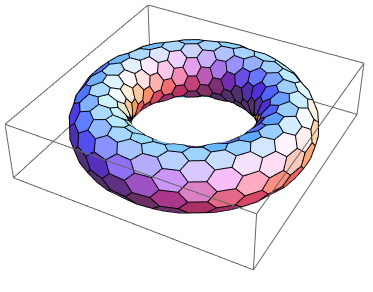
\includegraphics[width=0.75\textwidth]{images/test_image}
	\caption{The D-T Fusion Reaction} ~\\
	\small In a first generation tokamak reactor, the main source of energy will come from two hydrogen isotopes fusing into a helium particle -- and ejecting a 14.1 MeV neutron.
\end{figure}

The final point to make before returning to the fusion power derivation is the main difference between the two fusion products: helium (i.e. the alpha particle) and the neutron. First, neutrons lack a charge -- they are neutral. This means they cannot be confined with magnetic fields. As such, they simply move in straight lines until they collide with other particles. As the structure of a tokamak is mainly metal, the neutron is much more likely to collide there than the gaseous plasma, which is orders of magnitude less dense. Conversely, alpha particles are charged -- when stripped of their electrons -- and can therefore be kept within the plasma using magnets. What this means practically is that of the 17.6 MeV that comes from every fusion reaction, only 3.5 MeV remains inside the plasma (within the helium particle species).
 
 Returning to the problem at hand, the fusion power -- in megawatts -- is given in Jeff Freidberg's book through the following volume integral:
 
 \begin{equation}
 	\label{eq:pf_int}
 	P_F = \int E_F \, n_D \, n_T \, \langle \sigma v \rangle \, d \vec{\bold{r}}
 \end{equation}
 
 The $n_D$ and $n_T$ in this equation represent the density of the deuterium and tritium ions, respectively. Assuming a 50-50 mix of the two, they can be related to the electron density -- i.e. the one used in this model -- through the dilution factor:
 
 \begin{equation}
 	n_D = n_T = f_D \cdot \left( \frac{n}{2} \right)
 \end{equation}
 \myequations{Dilution Factor -- $f_{D}$}
 
 The fusion reactivity, $\langle \sigma v \rangle$, is then a nonlinear function of the temperature, T, which the model approximates using the Bosch-Hale tabulation (described in the appendix). As this tabulated value appears inside an integral, it seems important to point out that the temperature is now the most difficult floating variable to handle -- over $R_0$, $B_0$, $\overline n$, and $I_P$. This will come into play when the model is formalized next chapter.
 
 The next step in the derivation of fusion power is transforming the three-dimensional volume integral (see Eq. \ref{eq:pf_int}) into a one-dimensional radial one. First, the volume analogue of the previously given surface-area integral is:
 
 \begin{equation}
  	\label{eq:qv}
 	Q_V = 4 \pi^2 R_0 a^2 \kappa g \int_0^1 Q(\rho) \rho \, d\rho
 \end{equation}
 \myequations{Volume Integral -- $Q_V$}
 
 Where again, Q is an arbitrary function of $\rho$ and g is a geometric factor approximately equal to one. The fusion power can now be rewritten as:
 
 \begin{equation}
 	P_F = \pi^2 E_F f_D^2 R_0 a^2 \kappa g \int_0^1 n^2 \langle \sigma v \rangle \rho \, d\rho
 \end{equation}
 
 In standardized units, this becomes:
 
\begin{equation}
	\label{eq:pf}
	\tcboxmath{
	P_F = K_F \cdot \overline{n}^2 \cdot R_0^3  \cdot (\sigma v)
	}
\end{equation}
\myequations{Fusion Power -- $P_F$}

\begin{equation}
  K_F = 278.3 \cdot f_D^2 \cdot ( \epsilon^2 \kappa g )
\end{equation}

Where the standardized fusion reactivity is now,

\begin{equation}
   (\sigma v) = 10^{21} \, (1+\nu_n)^2 \int\limits_0^1 ( 1 - \rho^2 ) ^ { \, 2 \nu_n} \langle \sigma v \rangle \, \rho \, d\rho
\end{equation}

As mentioned before, this fusion power is divvied up 80-20 between the neutron and alpha particle. These relations will be used shortly. For now, they can be described mathematically as:

\begin{equation}
	P_\alpha = 0.2 \cdot P_F
\end{equation}
\myequations{Alpha Power -- $P_\alpha$}

\begin{equation}
	P_n = 0.8 \cdot P_F
\end{equation}
\myequations{Neutron Power -- $P_n$}

At this point, the current drive needed for steady-state can now be defined.

\subsection{Using Current Drive}

As may have been lost along the way, the current mission is to define a formula for steady current -- from the current balance equation for steady-state tokamaks in H-Mode:

\begin{equation}
		\tag{\ref{eq:ibal}}
		I_P = I_{BS} + I_{CD}
\end{equation}

In standardized units, the equation for the current drive is often given in the literature as: \cite{itercd}

\begin{equation}
	I_{CD} = \eta_{CD} \cdot \left( \frac{P_H}{\overline n R_0} \right)
\end{equation}

Here, $\eta_{CD}$ is the current drive efficiency with units $ \left(
\frac{ \textnormal{MA} }{ \textnormal{MW-m}^2 } \right) $ and $P_H$ is the heating power in megawatts driven by LHCD (and absorbed by the plasma).

Let it be known, though, that driving current in a plasma is hard. In fact, pulsed reactor designers (i.e. European fusion researchers) think it is so difficult, they may choose to forego it completely -- focusing only on inductive sources that necessitate reactor downtime. A common current drive efficiency ($\eta_{CD}$) seen in many designs is $0.3 \pm 0.1 $ in the standard units. It is however inherently a function of all the plasma parameters -- with subtlety put off until the discussion of self-consistency. For now it assumed to have some constant value.

The remaining step in deriving an equation for driven current ($I_{CD}$) is a formula for the heating power ($P_H$). The way fusion systems models -- like this one -- handle the heating power is through the physics gain factor, Q. Sometimes referred to as big Q, this value represents how many times over the heating power ($P_H$) is amplified as it is transformed into fusion power ($P_F$):

\begin{equation}
	P_H = \frac{P_F}{Q}
\end{equation}

Now, utilizing the previously defined Greenwald density and fusion power:

 \begin{equation}
 	\tag{\ref{eq:greenwald}}
 	\overline n = K_n \cdot \left( \frac{I_P}{R_0^2} \right)
 \end{equation}
 
 \begin{equation}
	\tag{\ref{eq:pf}}
	P_F = K_F \cdot \overline{n}^2 \cdot R_0^3  \cdot (\sigma v)
\end{equation}

The current from LHCD can be written as:

\begin{equation}
	\label{eq:icd}
	\tcboxmath{
	I_{CD} = K_{CD} \cdot I_P \cdot ( \sigma v )
	}
\end{equation}
\myequations{Current Drive -- $I_{CD}$}

\begin{equation}
	K_{CD} = \left( K_F K_n \right) \cdot \frac{\eta_{CD}}{Q}
\end{equation}

As $\eta_{CD}$ and Q appear within a fixed coefficient, it is implied that both remain constant throughout a solve. This subtlety is lifted when handling $\eta_{CD}$ self-consistently, which will be discussed shortly. However, even in that context, it proves beneficial to still think of $\eta_{CD}$ as a sequence of fixed variable.

\subsection{Completing the Steady Current}

As hinted along the way, the goal of this section has been to derive a simple formula for steady current ($I_P$). The problem started with current balance in a steady-state reactor:

\begin{equation}
	\tag{\ref{eq:ibal}}
	I_P = I_{BS} + I_{CD}
\end{equation}

Two equations were then found for the bootstrap ($I_{BS}$) and driven ($I_{CD}$) current:

\begin{equation}
	\tag{\ref{eq:ibs}}
	I_{BS} = K_{BS} \cdot \overline T
\end{equation}

\begin{equation}
	\tag{\ref{eq:icd}}
	I_{CD} = K_{CD} \cdot I_P \cdot ( \sigma v )
\end{equation}

Combining these three equations and solving for the total plasma current ($I_P$) -- in mega-amps -- yields:

\begin{equation}
	\label{eq:steady}
	\tcbhighmath{
	I_P = \frac{ K_{BS} \, \overline T }{ 1 - K_{CD} ( \sigma v ) }
	}
\end{equation}
\myequations{Steady Current -- $I_P$}

This is the answer we have been seeking!

As mentioned before, this simple formula appears to only depend on temperature! Apparently, the plasma should have the same current at some temperature (i.e. $\overline T$ = 15 keV), regardless of the size of the machine or the strength of its magnets. This has the important corollary that each temperature maps to only one current value. As has become a mantra, the subtlety of this behavior lies in the self-consistency of the current-drive efficiency -- $\eta_{CD}$.

\section{Handling Current Drive Self-Consistently}

Although a thorough description of the wave theory behind lower-hybrid current drive (LHCD) is well outside the scope of this text, it does motivate the solving of a tokamak's major radius ($R_0$) and field strength ($B_0$). It also shows how what was once a simple problem has now transformed into a rather complex one -- a common issue with plasmas.

The logic behind finding a self-consistent current-drive efficiency is starting at some plausible value (i.e. $\eta_{CD} = 0.3$), solving for the steady current -- i.e. $I_P = f(\overline T)$ -- and then somehow iteratively creeping towards a value deemed self-consistent. What this means is that in addition to the solver described in the last section, there needs to be a black-box function the solutions are piped through to get a better guesses at $\eta_{CD}$. The black-box function we use is a variation of the Ehst-Karney model. \cite{ehstkarney}

As mentioned, a self-consistent $\eta_{CD}$ is found once a trip through the Ehst-Karney black-box results in the same $\eta_{CD}$ as was piped in -- to some tolerable level of error. This consistency incorporates an explicit dependence on the tokamak configuration. Mathematically,

\begin{equation}
	\tilde \eta_{CD} = f( R_0, B_0, \overline n, \overline T, I_P )
\end{equation}
\myequations{Current Drive Efficiency -- $\eta_{CD}$}

As such, to recalculate it after every solution of the steady current requires a value for both $B_0$ and $R_0$ -- the targets of this model's primary and secondary constraints. These will be the highlight of the next chapter.

%\end{document}
